% ============================================================================
%  OMRiUS — udžbenik za pripremu obrane seminara i usmenog ispita
%  Krešimir Hartl, FSB, mentor prof. dr. sc. Andrej Jokić
%
%  Build:  python src/build_udzbenik.py     (Tectonic / XeTeX)
%  Boxes:  see preambula/okviri.tex — colour marks provenance only.
% ============================================================================
\documentclass[11pt,a4paper,oneside]{report}

% ============================================================================
%  stil.tex — fonts, page layout, headings, code listings
%  Engine: Tectonic (XeTeX) is canonical; pdfLaTeX fallback kept for MiKTeX.
%  The fontspec / newtxtext split is copied verbatim from docs/main.tex so the
%  textbook and the seminar render Croatian diacritics identically.
% ============================================================================

\usepackage{iftex}
\ifPDFTeX
  \usepackage[utf8]{inputenc}
  \usepackage[T1]{fontenc}
  \usepackage{newtxtext}
\else
  \usepackage{fontspec}
  \setmainfont{texgyretermes-regular.otf}[
    BoldFont       = texgyretermes-bold.otf,
    ItalicFont     = texgyretermes-italic.otf,
    BoldItalicFont = texgyretermes-bolditalic.otf
  ]
\fi
\usepackage[croatian]{babel}

\usepackage{amsmath,amssymb,mathtools}
\usepackage[top=2.4cm,bottom=2.4cm,left=2.6cm,right=2.6cm]{geometry}
\usepackage{setspace}
\onehalfspacing
\usepackage{microtype}
\usepackage{xcolor}
\usepackage{graphicx}
\usepackage{booktabs,tabularx,longtable,array,multirow}
\usepackage{float}
\usepackage{caption}
\usepackage{enumitem}
\usepackage{chngcntr}
\usepackage{fancyhdr}
\usepackage{titlesec}
\usepackage{listings}

\captionsetup[figure]{font={small,bf},labelsep=period,position=below}
\captionsetup[table]{font={small,bf},labelsep=period,position=above}

% Figures, tables and equations numbered per chapter: Slika 1.3, (2.7)
\counterwithin{figure}{chapter}
\counterwithin{table}{chapter}
\counterwithin{equation}{chapter}

\setcounter{secnumdepth}{3}
\setcounter{tocdepth}{2}

% --- Colours -----------------------------------------------------------------
\definecolor{fsbplava}{RGB}{0,51,102}
\definecolor{izvorcrvena}{RGB}{155,25,25}
\definecolor{zadatsiva}{RGB}{85,85,85}
\definecolor{seminarplava}{RGB}{20,70,140}
\definecolor{pojamzuta}{RGB}{150,110,0}
\definecolor{tihasiva}{RGB}{140,140,140}
\definecolor{zamkanarancasta}{RGB}{175,85,0}

% --- Headers and footers -----------------------------------------------------
\setlength{\headheight}{14pt}
\pagestyle{fancy}
\fancyhf{}
\fancyhead[L]{\small\itshape\nouppercase{\leftmark}}
\fancyhead[R]{\small\itshape OMRiUS — udžbenik za obranu}
\fancyfoot[C]{\small\bfseries\thepage}
\renewcommand{\headrulewidth}{0.4pt}
\renewcommand{\footrulewidth}{0pt}
\fancypagestyle{plain}{\fancyhf{}\fancyfoot[C]{\small\bfseries\thepage}%
  \renewcommand{\headrulewidth}{0pt}}

% --- Headings ----------------------------------------------------------------
\titleformat{\chapter}[display]
  {\normalfont\huge\bfseries\color{fsbplava}}
  {\filright\Large\chaptertitlename\ \thechapter}{12pt}{\Huge}
\titlespacing*{\chapter}{0pt}{-20pt}{28pt}
\titleformat{\section}
  {\normalfont\Large\bfseries\color{fsbplava}}{\thesection.}{0.5em}{}
\titleformat{\subsection}
  {\normalfont\large\bfseries}{\thesubsection.}{0.5em}{}
\titleformat{\subsubsection}
  {\normalfont\normalsize\bfseries\itshape}{\thesubsubsection.}{0.5em}{}

% --- Code listings (styles lifted from docs/main.tex) ------------------------
\lstdefinestyle{matlabstyle}{
  language=Matlab,
  basicstyle=\ttfamily\footnotesize,
  keywordstyle=\color{fsbplava}\bfseries,
  commentstyle=\color{teal}\itshape,
  stringstyle=\color{purple},
  numbers=left, numberstyle=\tiny\color{gray}, numbersep=8pt,
  breaklines=true, breakatwhitespace=false,
  showstringspaces=false, tabsize=2,
  frame=single, rulecolor=\color{gray!50},
  backgroundcolor=\color{black!3},
  columns=flexible,
  literate={č}{{\v c}}1 {ć}{{\'c}}1 {ž}{{\v z}}1 {š}{{\v s}}1 {đ}{{\dj}}1
           {Č}{{\v C}}1 {Ć}{{\'C}}1 {Ž}{{\v Z}}1 {Š}{{\v S}}1 {Đ}{{\DJ}}1
}
\lstdefinestyle{outputstyle}{
  basicstyle=\ttfamily\scriptsize,
  breaklines=true,
  frame=single, rulecolor=\color{gray!50},
  backgroundcolor=\color{black!4},
  columns=flexible,
  literate={č}{{\v c}}1 {ć}{{\'c}}1 {ž}{{\v z}}1 {š}{{\v s}}1 {đ}{{\dj}}1
           {Č}{{\v C}}1 {Ć}{{\'C}}1 {Ž}{{\v Z}}1 {Š}{{\v S}}1 {Đ}{{\DJ}}1
}
\renewcommand{\lstlistingname}{Ispis}

% ============================================================================
%  okviri.tex — the box system.
%
%  DESIGN RULE: colour marks PROVENANCE only — where the text came from.
%    red   = professor's lecture / exercise slide, verbatim
%    grey  = the assignment text, verbatim, nothing added
%    blue  = the seminar v1.2 solution, verbatim
%    yellow= a definition or formula worth memorising
%  Everything else (derivation steps, traps, exam questions) stays QUIET:
%  a thin rule, no fill. Otherwise the page turns into a colour salad and the
%  reader loses the one signal that matters — "is this mine or the professor's?"
% ============================================================================

\usepackage[most]{tcolorbox}
\tcbuselibrary{skins,breakable}

\newcommand{\okvirnaslov}[2]{\textcolor{#1}{\textbf{\footnotesize\MakeUppercase{#2}}}}

% --- RED: verbatim from the lecture / exercise slides ------------------------
% #1 = precise reference, e.g. "Vježbe 3, slajd 18/36 (PDF str. 23)"
\newtcolorbox{izvor}[1]{
  breakable, enhanced,
  colback=izvorcrvena!3, colframe=izvorcrvena,
  boxrule=1.1pt, arc=1.5pt, left=8pt, right=8pt, top=7pt, bottom=7pt,
  title={\footnotesize\bfseries S PREDAVANJA / VJEŽBI \;—\; #1},
  fonttitle=\color{white}, coltitle=white,
  attach boxed title to top left={xshift=8pt, yshift=-9pt},
  boxed title style={colback=izvorcrvena, boxrule=0pt, arc=1pt}
}

% --- GREY: verbatim assignment text. Nothing derived may enter this box. -----
\newtcolorbox{zadatak}[1]{
  breakable, enhanced,
  colback=black!4, colframe=zadatsiva,
  boxrule=1.1pt, arc=1.5pt, left=8pt, right=8pt, top=7pt, bottom=7pt,
  title={\footnotesize\bfseries IZVORNI TEKST ZADATKA \;—\; #1},
  coltitle=white,
  attach boxed title to top left={xshift=8pt, yshift=-9pt},
  boxed title style={colback=zadatsiva, boxrule=0pt, arc=1pt}
}

% --- BLUE: verbatim from the seminar v1.2 ------------------------------------
\newtcolorbox{seminar}[1]{
  breakable, enhanced,
  colback=seminarplava!4, colframe=seminarplava,
  boxrule=1.1pt, arc=1.5pt, left=8pt, right=8pt, top=7pt, bottom=7pt,
  title={\footnotesize\bfseries KAKO JE RIJEŠENO U SEMINARU \;—\; #1},
  coltitle=white,
  attach boxed title to top left={xshift=8pt, yshift=-9pt},
  boxed title style={colback=seminarplava, boxrule=0pt, arc=1pt}
}

% --- YELLOW: definitions and formulas to memorise ----------------------------
\newtcolorbox[auto counter, number within=chapter]{pojam}[1]{
  breakable, enhanced,
  colback=yellow!8, colframe=pojamzuta,
  boxrule=1.1pt, arc=1.5pt, left=8pt, right=8pt, top=7pt, bottom=7pt,
  title={\footnotesize\bfseries DEFINICIJA \thetcbcounter \;—\; #1},
  coltitle=white,
  attach boxed title to top left={xshift=8pt, yshift=-9pt},
  boxed title style={colback=pojamzuta, boxrule=0pt, arc=1pt}
}
\newtcolorbox[auto counter, number within=chapter]{formula}[1]{
  breakable, enhanced,
  colback=yellow!8, colframe=pojamzuta,
  boxrule=1.1pt, arc=1.5pt, left=8pt, right=8pt, top=7pt, bottom=7pt,
  title={\footnotesize\bfseries FORMULA \thetcbcounter \;—\; #1},
  coltitle=white,
  attach boxed title to top left={xshift=8pt, yshift=-9pt},
  boxed title style={colback=pojamzuta, boxrule=0pt, arc=1pt}
}

% ============================================================================
%  QUIET elements — no fill, thin rule on the left only.
% ============================================================================

% What you must already know before reading on.
\newtcolorbox{predznanje}{
  breakable, enhanced, colback=white, colframe=white,
  borderline west={2pt}{0pt}{tihasiva},
  boxrule=0pt, sharp corners, left=10pt, right=0pt, top=4pt, bottom=4pt,
  before upper={\textcolor{tihasiva}{\footnotesize\bfseries ŠTO MORAŠ ZNATI PRIJE}\par\smallskip}
}

% One numbered step of a derivation, or a run of them.
\newtcolorbox{korak}[1][Izvod korak po korak]{
  breakable, enhanced, colback=white, colframe=white,
  borderline west={2pt}{0pt}{fsbplava!45},
  boxrule=0pt, sharp corners, left=10pt, right=0pt, top=4pt, bottom=4pt,
  before upper={\textcolor{fsbplava}{\footnotesize\bfseries\MakeUppercase{#1}}\par\smallskip}
}

% A mistake that is actually made, and why it is wrong.
\newtcolorbox{zamka}[1][Zamka]{
  breakable, enhanced, colback=white, colframe=white,
  borderline west={2pt}{0pt}{zamkanarancasta},
  boxrule=0pt, sharp corners, left=10pt, right=0pt, top=4pt, bottom=4pt,
  before upper={\textcolor{zamkanarancasta}{\footnotesize\bfseries\MakeUppercase{#1}}\par\smallskip}
}

% Examiner's question + model answer.
\newtcolorbox{pitanje}[1]{
  breakable, enhanced, colback=white, colframe=black!35,
  boxrule=0.5pt, sharp corners, left=8pt, right=8pt, top=6pt, bottom=6pt,
  before upper={\textbf{Pitanje.} \emph{#1}\par\smallskip}
}

% How to draw it on the blackboard, by hand, in front of the examiner.
\newtcolorbox{ploca}[1][Crtanje na ploči — korak po korak]{
  breakable, enhanced, colback=white, colframe=white,
  borderline west={2pt}{0pt}{teal!60},
  boxrule=0pt, sharp corners, left=10pt, right=0pt, top=4pt, bottom=4pt,
  before upper={\textcolor{teal!70!black}{\footnotesize\bfseries\MakeUppercase{#1}}\par\smallskip}
}

% What to say out loud. Verbatim sentences.
\newtcolorbox{izgovor}[1][Kako to reći naglas]{
  breakable, enhanced, colback=white, colframe=white,
  borderline west={2pt}{0pt}{violet!50},
  boxrule=0pt, sharp corners, left=10pt, right=0pt, top=4pt, bottom=4pt,
  before upper={\textcolor{violet!70!black}{\footnotesize\bfseries\MakeUppercase{#1}}\par\smallskip}
}

% ============================================================================
%  Helpers
% ============================================================================
% \slajd{id}{width fraction} — inserts a rendered slide page from slides/.
\newcommand{\slajd}[2][0.92]{%
  \begin{center}%
    \fbox{\includegraphics[width=#1\linewidth]{slides/#2.png}}%
  \end{center}%
}
% \skenzad{id} — a rendered page/crop of the original assignment scan.
\newcommand{\skenzad}[2][0.92]{%
  \begin{center}%
    \fbox{\includegraphics[width=#1\linewidth]{zadatak/#2.png}}%
  \end{center}%
}

% ============================================================================
%  makroi.tex — notation macros. One definition per concept so the whole book
%  stays consistent with the professor's notation (Gx - h <= 0, theta(mu), v).
% ============================================================================

\providecommand{\coloneqq}{\mathrel{\vcentcolon=}}

\newcommand{\R}{\mathbb{R}}                      % real numbers
\newcommand{\Rn}[1]{\mathbb{R}^{#1}}
\newcommand{\Sym}[1]{\mathbb{S}^{#1}}            % symmetric matrices
\newcommand{\trans}{^{\mathsf{T}}}               % transpose
\newcommand{\grad}{\nabla}
\newcommand{\Lag}{\mathcal{L}}                   % Lagrangian
\newcommand{\dual}{\theta}                       % dual function theta(mu)
\newcommand{\feas}{\mathcal{F}}                  % feasible set
\newcommand{\popt}{p^{\star}}                    % optimal primal value
\newcommand{\dopt}{d^{\star}}                    % optimal dual value
\newcommand{\xopt}{x^{\star}}
\newcommand{\muopt}{\mu^{\star}}
\newcommand{\psd}{\succeq}                       % positive semidefinite
\newcommand{\pd}{\succ}                          % positive definite
\newcommand{\nsd}{\preceq}
\newcommand{\nd}{\prec}
\newcommand{\norm}[1]{\left\lVert #1 \right\rVert}
\newcommand{\abs}[1]{\left\lvert #1 \right\rvert}
\newcommand{\inner}[2]{\left\langle #1,\, #2 \right\rangle}
\newcommand{\diag}{\operatorname{diag}}
\newcommand{\eig}{\operatorname{eig}}
\newcommand{\rank}{\operatorname{rank}}
\newcommand{\tr}{\operatorname{tr}}
\newcommand{\Real}{\operatorname{Re}}
\newcommand{\dom}{\operatorname{dom}}
\newcommand{\dd}{\,\mathrm{d}}               % differential in integrals
\newcommand{\subjto}{\text{uz ograničenja}}

% Reference to a page in Part 0 where a symbol is introduced.
\newcommand{\vidi}[1]{\textcolor{tihasiva}{\footnotesize(vidi str.~\pageref{#1})}}


\usepackage[hidelinks,unicode]{hyperref}
\hypersetup{
  pdftitle={OMRiUS — udžbenik za pripremu obrane seminara},
  pdfauthor={Krešimir Hartl},
  bookmarksnumbered=true
}

\graphicspath{{./}{figures/}{../figures/}}

\begin{document}

% ---------------------------------------------------------------- title page
\begin{titlepage}
\centering
\vspace*{1.5cm}
{\large Sveučilište u Zagrebu\par\smallskip Fakultet strojarstva i brodogradnje\par}
\vspace{2.5cm}
{\Huge\bfseries\color{fsbplava} OPTIMIZACIJSKE METODE\par\vspace{0.3cm}
 U RAZVOJU I UPRAVLJANJU SUSTAVA\par}
\vspace{1.2cm}
{\LARGE Udžbenik za pripremu obrane seminarskog rada\par}
\vspace{0.6cm}
{\large\itshape Zadatak po zadatak, od nule, s izvorima uz svaku tvrdnju\par}
\vspace{2.5cm}
\begin{tabular}{rl}
\textbf{Student:} & Krešimir Hartl \\[4pt]
\textbf{Mentor:} & Prof.\ dr.\ sc.\ Andrej Jokić \\[4pt]
\textbf{Temelj:} & Seminarski rad v1.2 \\[4pt]
\textbf{Izvori:} & Predavanja 1--8, Vježbe 1--5 \\
\end{tabular}
\vfill
{\large Zagreb, \today\par}
\end{titlepage}

% ---------------------------------------------------------------------- toc
\pagenumbering{roman}
\tableofcontents
\clearpage
\pagenumbering{arabic}

% ------------------------------------------------------------------- part 0
\part*{Dio 0 — prije nego išta počneš računati}
\addcontentsline{toc}{part}{Dio 0 — prije nego išta počneš računati}
\chapter{Kako se ovaj udžbenik koristi}
\label{ch:kako-koristiti}

\section{Čemu ovaj udžbenik služi}

Ovaj udžbenik ima jedan zadatak: da s minimalnim predznanjem možeš u cijelosti
razumjeti i obraniti seminarski rad iz kolegija \emph{Optimizacijske metode u razvoju i
upravljanju sustava}. Ne pretpostavlja da već znaš što je euklidski prostor, što znači
$\langle x, y \rangle$ ili zašto se piše $\coloneqq$ umjesto $=$. Sve se to definira
prije prve upotrebe, u Poglavlju~\ref{ch:rjecnik}.

Građen je \textbf{po zadacima}, ne po temama. Ideš zadatak po zadatak, podzadatak po
podzadatak, točno onim redom kojim ćeš ih morati izložiti na obrani. Teorija ulazi
onda kad zatreba i tamo gdje zatreba --- ne prije.

\section{Četiri boje: odakle koji tekst dolazi}

Najveći problem pri učenju iz vlastitih bilježaka jest da se poslije ne zna
\emph{tko je što rekao}: je li ovo profesorova definicija, je li ovo bio dio zadatka,
ili sam to sâm zaključio. Zato u ovom udžbeniku \textbf{boja označava isključivo
podrijetlo teksta}, ništa drugo.

\begin{izvor}{Predavanje 2 --- Definicije, klasifikacija, konveksnost, slajd 60/71 (PDF str.~61)}
Crveni okvir je doslovno ono što piše na profesorovu slajdu. Stranica slajda umeće se
kao slika, pa ispod nje slijedi pretipkani sadržaj s objašnjenjem svakog simbola.
Referenca uvijek ima \emph{dva} broja: broj slajda ispisan u podnožju samog slajda i
broj stranice u PDF-u. Ta se dva broja razlikuju, jer beamer svaki slajd s postupnim
otkrivanjem sprema kao više PDF stranica.

\slajd{p02-konveksna-funkcija}
\end{izvor}

\begin{zadatak}{Zadatak 1, uvodna formulacija}
Sivi okvir je doslovni tekst zadatka --- izravno sa skena koji je profesor potpisao.
Unutar sivog okvira \textbf{nema} ničega što je netko poslije dodao, zaključio ili
protumačio. Ako nešto u zadatku nije rečeno, u sivom okviru toga neće biti.
\skenzad[0.98]{z1-original}
\end{zadatak}

\begin{seminar}{Seminar v1.2, §1.1}
Plavi okvir je doslovni izvadak iz predanog seminarskog rada v1.2 --- ista notacija,
iste jednadžbe, isti brojevi kao u PDF-u koji je predan. Tako uvijek znaš što točno
braniš.
\end{seminar}

\begin{pojam}{Konveksna funkcija}
Žuti okvir je definicija ili formula koju treba znati napamet. Numeriran je, pa se na
njega poslije referira brojem.

Funkcija $f: S \to \R$ je \textbf{konveksna} ako je $S$ konveksan skup i ako za sve
$x_1, x_2 \in S$ te za svaki $\alpha$, $0 < \alpha < 1$, vrijedi
\begin{equation}
f\bigl(\alpha x_1 + (1-\alpha) x_2\bigr) \;\leq\; \alpha f(x_1) + (1-\alpha) f(x_2).
\end{equation}
\end{pojam}

\section{Tihi elementi}

Sve što nije jedan od ta četiri okvira nema ispunu ni boju --- samo tanku crtu s lijeve
strane. To je namjerno: da četiri boje ostanu jedini glasan signal na stranici.

\begin{predznanje}
\begin{itemize}[nosep,leftmargin=*]
  \item Popis simbola i pojmova koje moraš znati prije nego kreneš dalje.
  \item Uz svaki stoji stranica na kojoj je objašnjen.
\end{itemize}
\end{predznanje}

\begin{korak}
Numerirani izvod. Svaki korak imenuje simbole koje uvodi; nijedan algebarski korak se
ne preskače uz \emph{očito slijedi}.
\begin{enumerate}[nosep,leftmargin=*]
  \item Zapiši ono što znaš.
  \item Uvrsti.
  \item Zaključi, i reci \emph{zašto} smiješ zaključiti.
\end{enumerate}
\end{korak}

\begin{zamka}
Greška koja se stvarno radi, i objašnjenje zašto je pogrešna. Nije popis općenitih
savjeta nego konkretan promašaj koji te na obrani može stajati ocjene.
\end{zamka}

\begin{ploca}
Kako nacrtati sliku rukom, na ploči, bez računala: koje osi, kojim redom, koje točke
označiti i što napisati uz njih.
\end{ploca}

\begin{izgovor}
Doslovne rečenice koje možeš izgovoriti pred ispitivačem. Nisu parafraza --- napisane
su tako da ih se može reći od riječi do riječi.
\end{izgovor}

\begin{pitanje}{Zašto je Hesseova matrica ovdje konstantna?}
Okvir s pitanjem ispitivača, a odmah ispod modelski odgovor.

\textbf{Odgovor.} Jer je funkcija cilja kvadratna: druge parcijalne derivacije
kvadratne funkcije su konstante, pa Hesseova matrica ne ovisi o $x$.
\end{pitanje}

\section{Ritam svakog podzadatka}

Svaki podzadatak --- 1a, 1b, \dots, 4c --- ide istim redom od devet koraka. Kad se
navikneš na taj ritam, znaš gdje ćeš što naći bez traženja.

\begin{enumerate}[leftmargin=*]
  \item \textbf{Što se traži} --- jedna rečenica, bez žargona.
  \item \textbf{Sivi okvir} --- izvorni tekst zadatka.
  \item \textbf{Predznanje} --- što moraš znati prije, sa stranicama.
  \item \textbf{Crveni okvir} --- slajd s predavanja ili vježbi, pa transkripcija.
  \item \textbf{Žuti okviri} --- definicije i formule koje se koriste.
  \item \textbf{Izvod korak po korak} --- bez preskakanja.
  \item \textbf{Plavi okvir} --- kako je riješeno u seminaru.
  \item \textbf{Graf} --- slika, čitanje slike, crtanje rukom.
  \item \textbf{MATLAB i stvarni ispis} --- kod i doslovni ispis programa.
\end{enumerate}

Na kraju svakog zadatka slijedi modul za obranu: pitanja, zamke i modelski odgovori.

\section{Jedno upozorenje o izvornom tekstu zadatka}

Uz zadatak u repozitoriju postoji i prijepis
(\texttt{TASK/zadatak\_omrius.md}) u kojem uz svaki podzadatak stoji i numerirani popis
\emph{Koraka rješavanja}. Ti koraci \textbf{nisu} profesorov tekst --- dopisani su
naknadno kao pomoć pri radu. U ovom udžbeniku oni nikad ne ulaze u sivi okvir. Kad se
koriste, izričito su označeni kao izvedena uputa, a ne kao dio zadatka.

\chapter{Rječnik: svaki znak, kako se čita i što znači}
\label{ch:rjecnik}

Ovo poglavlje postoji zato što se u matematičkom tekstu ništa ne smije
podrazumijevati. Svaki znak koji se pojavljuje bilo gdje u ovom udžbeniku, u
seminaru ili na predavanjima ovdje ima svoj redak: kako se piše, \textbf{kako se
čita naglas}, što znači i gdje ga prvi put susrećeš.

Čitanje naglas nije ukras. Na usmenoj obrani ne pokazuješ prstom u simbol nego
ga izgovaraš, i ispitivač po tome odmah čuje razumiješ li ga ili si ga zapamtio
kao sliku.

\section{Znakovi kojima se nešto definira ili tvrdi}
\label{sec:znakovi-logike}

\begin{longtable}{@{}p{0.13\linewidth} p{0.27\linewidth} p{0.52\linewidth}@{}}
\toprule
\textbf{Zapis} & \textbf{Kako se čita} & \textbf{Što znači} \\
\midrule
\endfirsthead
\toprule
\textbf{Zapis} & \textbf{Kako se čita} & \textbf{Što znači} \\
\midrule
\endhead
$\coloneqq$ & ,,definira se kao`` & Lijeva strana je \emph{novo ime} koje ovime uvodimo za ono što piše desno. Nije tvrdnja da su dvije poznate stvari jednake, nego uvođenje oznake. Piše se dvotočka pa znak jednakosti. \\[4pt]
$=$ & ,,jednako je`` & Tvrdnja da dvije već poznate veličine imaju istu vrijednost. \\[4pt]
$\equiv$ & ,,identički je jednako`` & Jednakost koja vrijedi za \emph{svaku} vrijednost varijable, ne samo za neke. \\[4pt]
$\implies$ & ,,povlači``, ,,slijedi`` & Ako vrijedi lijevo, onda nužno vrijedi i desno. \\[4pt]
$\iff$ & ,,ako i samo ako`` & Vrijedi u oba smjera: lijevo povlači desno \emph{i} desno povlači lijevo. \\[4pt]
$\forall$ & ,,za svaki`` & Tvrdnja vrijedi za sve elemente nekog skupa bez iznimke. \\[4pt]
$\exists$ & ,,postoji`` & Postoji barem jedan element s traženim svojstvom. \\[4pt]
$\in$ & ,,je element skupa``, kraće ,,pripada`` & $x \in S$: objekt $x$ je jedan od članova skupa $S$. \\[4pt]
$\subset$ & ,,je podskup od`` & Svaki element lijevog skupa je i element desnog. \\[4pt]
$\cap$ & ,,presjek`` & Skup onih elemenata koji su u \emph{oba} skupa istovremeno. \\[4pt]
$\cup$ & ,,unija`` & Skup onih elemenata koji su u barem jednom od skupova. \\[4pt]
$\{x \mid P(x)\}$ & ,,skup svih $x$ takvih da vrijedi $P$ od $x$`` & Uspravna crta se čita ,,takav da``. Ovako se zapisuju svi dopustivi skupovi u ovom kolegiju. \\
\bottomrule
\end{longtable}

\begin{zamka}[Zamka: $\coloneqq$ nasuprot $=$]
Studenti često pišu $=$ tamo gdje bi trebalo $\coloneqq$ i obrnuto. Razlika je
sadržajna, ne kozmetička. Kad napišeš
\[
\Lag(x,\mu) \coloneqq f(x) + \mu\trans\bigl(Gx - h\bigr),
\]
ti \emph{uvodiš} Lagrangeovu funkciju --- prije te rečenice ona ne postoji. Kad
poslije napišeš $\grad_x \Lag(x,\mu) = 0$, to je \emph{uvjet} koji tražiš da bude
zadovoljen. Ako oboje napišeš s $=$, iz zapisa se više ne vidi što je definicija,
a što tvrdnja koju treba dokazati.
\end{zamka}

\section{Brojevi, prostori i skupovi}
\label{sec:prostori}

\begin{longtable}{@{}p{0.15\linewidth} p{0.30\linewidth} p{0.47\linewidth}@{}}
\toprule
\textbf{Zapis} & \textbf{Kako se čita} & \textbf{Što znači} \\
\midrule
\endfirsthead
\toprule
\textbf{Zapis} & \textbf{Kako se čita} & \textbf{Što znači} \\
\midrule
\endhead
$\R$ & ,,er`` ili ,,skup realnih brojeva`` & Svi realni brojevi: cijeli, razlomci i iracionalni, od $-\infty$ do $+\infty$. \\[4pt]
$\R^n$ & ,,er na en`` & Skup svih uređenih $n$-torki realnih brojeva. Element od $\R^2$ je par $(x_1, x_2)$, npr.\ točka u ravnini. \\[4pt]
$\R^{n \times m}$ & ,,er na en puta em`` & Skup svih matrica s $n$ redaka i $m$ stupaca, s realnim elementima. \\[4pt]
$\Sym{n}$ & ,,es na en``, ,,skup simetričnih matrica reda en`` & Sve realne kvadratne matrice $n \times n$ koje su simetrične, $M = M\trans$. Hesseova matrica uvijek pripada ovom skupu. \\[4pt]
$\R_{+}$ & ,,er plus`` & Nenegativni realni brojevi, $\{x \in \R \mid x \geq 0\}$. Lagrangeovi množitelji nejednakosti žive ovdje. \\[4pt]
$[0, L]$ & ,,zatvoreni interval od nula do el`` & Svi realni brojevi između $0$ i $L$, \emph{uključivo} s rubovima. Uglata zagrada znači da je rub uključen. \\[4pt]
$\emptyset$ & ,,prazan skup`` & Skup bez ijednog elementa. Ako je dopustivi skup prazan, problem nema rješenja. \\[4pt]
$\feas$ & ,,ef``, ,,dopustivi skup`` & Skup svih $x$ koji zadovoljavaju sva ograničenja problema. \\
\bottomrule
\end{longtable}

\subsection{Što je zapravo euklidski prostor}
\label{sec:euklidski}

Izraz ,,euklidski prostor`` u udžbenicima se često baci bez objašnjenja, pa ga
ovdje razlažemo do kraja.

\begin{korak}[Od skupa do euklidskog prostora]
\begin{enumerate}[leftmargin=*]
  \item Kreni od skupa $\R^n$. To je zasad samo \emph{popis} $n$-torki brojeva:
        $(1,\,2)$, $(-3,\,0{,}5)$ i tako dalje. Ništa u tom popisu još ne govori
        o duljini, kutu ili udaljenosti.
  \item Dodaj \textbf{zbrajanje} i \textbf{množenje skalarom}, oboje po
        komponentama:
        $x + y = (x_1+y_1, \dots, x_n+y_n)$ i $\alpha x = (\alpha x_1, \dots, \alpha x_n)$.
        Time $\R^n$ postaje \emph{vektorski prostor}: elementi se mogu zbrajati i
        rastezati, pa ih zovemo vektorima.
  \item Dodaj \textbf{skalarni produkt} $\inner{x}{y} = \sum_{i=1}^{n} x_i y_i$.
        Tek s njim možeš izraziti duljinu, $\norm{x} = \sqrt{\inner{x}{x}}$, i kut
        između dva vektora.
  \item Vektorski prostor $\R^n$ opremljen upravo tim skalarnim produktom zove se
        \textbf{euklidski prostor}. ,,Euklidski`` znači da u njemu vrijedi
        uobičajena geometrija iz škole: Pitagorin poučak, pravci, kutovi, okomitost.
\end{enumerate}
\end{korak}

\begin{izgovor}
,,Projektne varijable su vektor iz $\R^2$, dakle iz dvodimenzionalnog euklidskog
prostora --- to je obična ravnina sa standardnim skalarnim produktom, pa smijem
crtati dopustivi skup i nivo-krivulje u koordinatnom sustavu i sve što na slici
vidim kao okomitost stvarno jest okomitost.``
\end{izgovor}

\begin{pojam}{Skalarni produkt}
Za $x, y \in \R^n$ \textbf{skalarni produkt} je broj
\begin{equation}
\inner{x}{y} \;\coloneqq\; x\trans y \;=\; \sum_{i=1}^{n} x_i y_i .
\label{eq:skalarni-produkt}
\end{equation}
Čita se: ,,skalarni produkt od $x$ i $y$``, ili ,,iks transponirano ipsilon``.
Rezultat je \emph{jedan broj}, ne vektor --- odatle naziv ,,skalarni``.

Tri stvari koje iz njega slijede i koje se koriste kroz cijeli kolegij:
\begin{itemize}[nosep,leftmargin=*]
  \item \textbf{duljina}: $\norm{x} = \sqrt{\inner{x}{x}}$;
  \item \textbf{okomitost}: $x \perp y$ točno kad je $\inner{x}{y} = 0$;
  \item \textbf{projekcija i kut}: $\inner{x}{y} = \norm{x}\,\norm{y}\cos\varphi$,
        gdje je $\varphi$ kut između $x$ i $y$.
\end{itemize}
\end{pojam}

Zašto je to važno baš ovdje: ograničenje $a\trans x \leq b$ je izjava o skalarnom
produktu. Skup točaka za koje je $a\trans x = b$ je pravac (u ravnini) ili
hiperravnina (općenito), a vektor $a$ je na taj pravac \emph{okomit}. Zato se
gradijenti ograničenja na slici uvijek crtaju kao strelice okomite na pripadni
rubni pravac.

\section{Vektori i matrice}
\label{sec:vektori-matrice}

\begin{longtable}{@{}p{0.15\linewidth} p{0.30\linewidth} p{0.47\linewidth}@{}}
\toprule
\textbf{Zapis} & \textbf{Kako se čita} & \textbf{Što znači} \\
\midrule
\endfirsthead
\toprule
\textbf{Zapis} & \textbf{Kako se čita} & \textbf{Što znači} \\
\midrule
\endhead
$x$ & ,,iks``, ,,vektor iks`` & Vektor projektnih (odlučivačkih) varijabli. U ovom kolegiju uvijek \emph{stupčani} vektor. \\[4pt]
$x_i$ & ,,iks i-ti`` & $i$-ta komponenta vektora $x$, dakle jedan broj. \\[4pt]
$x\trans$ & ,,iks transponirano`` & Stupac pretvoren u redak. Potreban da bi umnožak $x\trans y$ bio broj. \\[4pt]
$\inner{x}{y}$ & ,,skalarni produkt iks i ipsilon`` & Isto što i $x\trans y$; vidi \eqref{eq:skalarni-produkt}. \\[4pt]
$\norm{x}$ & ,,norma od iks`` & Duljina vektora. Bez indeksa podrazumijeva se euklidska norma $\norm{x}_2$. \\[4pt]
$\norm{x}_1$ & ,,el jedan norma od iks`` & Zbroj apsolutnih vrijednosti, $\sum_i \abs{x_i}$. Ovo je funkcija cilja u Zadatku 3. \\[4pt]
$I$ & ,,jedinična matrica`` & Kvadratna matrica s jedinicama na dijagonali i nulama izvan nje. \\[4pt]
$Q, G, A, B$ & ,,ku``, ,,ge``, ,,a``, ,,be`` & Matrice; velika slova. $Q$ je matrica kvadratnog člana, $G$ matrica ograničenja, $A$ i $B$ matrice dinamike sustava. \\[4pt]
$\det(M)$ & ,,determinanta od em`` & Broj pridružen kvadratnoj matrici. $\det(M) = 0$ znači da je matrica singularna, tj.\ da njen inverz ne postoji. \\[4pt]
$M^{-1}$ & ,,em inverz`` & Matrica za koju je $M M^{-1} = I$. Postoji točno kad je $\det(M) \neq 0$. \\[4pt]
$\eig(M)$ & ,,svojstvene vrijednosti od em`` & Brojevi $\lambda$ za koje $\det(\lambda I - M) = 0$. Za simetrične matrice uvijek realni. \\[4pt]
$\lambda_i$ & ,,lambda i-ta`` & $i$-ta svojstvena vrijednost. \\[4pt]
$\tr(M)$ & ,,trag od em`` & Zbroj dijagonalnih elemenata; ujedno zbroj svih svojstvenih vrijednosti. \\[4pt]
$\diag(v)$ & ,,dijagonalna matrica od ve`` & Matrica kojoj su na dijagonali komponente vektora $v$, a svugdje drugdje nule. \\
\bottomrule
\end{longtable}

\subsection{Uspoređivanje: četiri različita znaka za ,,manje``}
\label{sec:relacije}

Ovo je mjesto gdje se najviše griješi, jer četiri vizualno slična znaka znače
četiri različite stvari.

\begin{longtable}{@{}p{0.13\linewidth} p{0.30\linewidth} p{0.49\linewidth}@{}}
\toprule
\textbf{Zapis} & \textbf{Kako se čita} & \textbf{Što znači} \\
\midrule
\endfirsthead
\toprule
\textbf{Zapis} & \textbf{Kako se čita} & \textbf{Što znači} \\
\midrule
\endhead
$a \leq b$ & ,,a manje ili jednako be`` & Usporedba \emph{dva broja}. \\[4pt]
$x \leq y$ (vektori) & ,,iks manje ili jednako ipsilon, po komponentama`` & Vrijedi $x_i \leq y_i$ za \emph{svaki} $i$. Tako se čita $Gx - h \leq 0$: svaki redak posebno. \\[4pt]
$M \psd 0$ & ,,em je pozitivno semidefinitna`` & $M$ je simetrična i sve su joj svojstvene vrijednosti $\geq 0$. Ekvivalentno: $z\trans M z \geq 0$ za svaki $z$. \\[4pt]
$M \pd 0$ & ,,em je pozitivno definitna`` & Sve svojstvene vrijednosti strogo $> 0$; ekvivalentno $z\trans M z > 0$ za svaki $z \neq 0$. \\[4pt]
$M \nd 0$ & ,,em je negativno definitna`` & Sve svojstvene vrijednosti strogo $< 0$. Ovako se zapisuju Ljapunovljeve nejednakosti u Zadatku 4. \\
\bottomrule
\end{longtable}

\begin{zamka}[Zamka: $\psd$ nije $\geq$ po elementima]
$M \psd 0$ \emph{ne} znači da su svi elementi matrice nenegativni. Matrica
\[
Q = \begin{bmatrix} 2 & -0.3 \\ -0.3 & 4 \end{bmatrix}
\]
iz Zadatka 1 ima negativan element $-0{,}3$, a ipak je pozitivno definitna, jer
su joj obje svojstvene vrijednosti pozitivne. Profesor to izričito naglašava na
slajdu: ,,Pozitivno definitne matrice mogu imati negativne elemente!``\ Obrnuto
također vrijedi --- matrica sa samim pozitivnim elementima može biti
indefinitna.
\end{zamka}

\begin{izvor}{Predavanje 2 --- Definicije, klasifikacija, konveksnost, slajd 46/71 (PDF str.~47)}
\slajd[0.86]{p02-psd-svojstvene}

\textbf{Što ovdje piše, redak po redak:}
\begin{itemize}[nosep,leftmargin=*]
  \item Simetrične matrice nužno imaju samo realne svojstvene vrijednosti ---
        zato kod provjere definitnosti nikad ne moraš računati s kompleksnim
        brojevima.
  \item $H \psd 0$ ako i samo ako su sve svojstvene vrijednosti nenegativne;
        $H \pd 0$ ako i samo ako su sve strogo pozitivne; analogno za
        $\nsd$ i $\nd$ s nepozitivnima i negativnima.
  \item Dvije napomene koje profesor posebno ističe: ako matrica nije pozitivno
        semidefinitna, to \emph{ne} znači da je negativno definitna (može biti
        ni jedno ni drugo, tzv.\ indefinitna); i --- pozitivno definitne matrice
        smiju imati negativne elemente.
\end{itemize}
\end{izvor}

\section{Derivacije, gradijent i Hesseova matrica}
\label{sec:derivacije-oznake}

\begin{longtable}{@{}p{0.17\linewidth} p{0.30\linewidth} p{0.45\linewidth}@{}}
\toprule
\textbf{Zapis} & \textbf{Kako se čita} & \textbf{Što znači} \\
\midrule
\endfirsthead
\toprule
\textbf{Zapis} & \textbf{Kako se čita} & \textbf{Što znači} \\
\midrule
\endhead
$\frac{\partial f}{\partial x_i}$ & ,,parcijalna derivacija ef po iks i-tom`` & Derivacija po jednoj varijabli, dok se sve ostale drže konstantnima. \\[4pt]
$\grad f(x)$ & ,,gradijent od ef u točki iks``, ili ,,nabla ef`` & Stupčani vektor svih prvih parcijalnih derivacija. Pokazuje smjer najbržeg rasta funkcije. \\[4pt]
$\grad^2 f(x)$ & ,,Hesseova matrica`` ili ,,nabla kvadrat ef`` & Matrica svih drugih parcijalnih derivacija. Za dva puta neprekidno derivabilne funkcije je simetrična. \\[4pt]
$\grad_x \Lag$ & ,,gradijent Lagrangiana po iks`` & Gradijent uzet samo po varijablama $x$, dok se $\mu$ drži fiksnim. Indeks govori po čemu se derivira. \\[4pt]
$\dot{x}(t)$ & ,,iks točka od te`` & Derivacija po vremenu, $\mathrm{d}x/\mathrm{d}t$. Točka iznad slova \emph{uvijek} znači derivaciju po vremenu. \\[4pt]
$\lfloor t \rfloor$ & ,,najveće cijelo od te`` & Najveći cijeli broj koji nije veći od $t$: $\lfloor 2{,}7 \rfloor = 2$. Ovime se u Zadatku 4 zadaje trenutak preklapanja. \\
\bottomrule
\end{longtable}

\section{Oznake optimizacijskog problema}
\label{sec:oznake-optimizacije}

\begin{longtable}{@{}p{0.14\linewidth} p{0.30\linewidth} p{0.48\linewidth}@{}}
\toprule
\textbf{Zapis} & \textbf{Kako se čita} & \textbf{Što znači} \\
\midrule
\endfirsthead
\toprule
\textbf{Zapis} & \textbf{Kako se čita} & \textbf{Što znači} \\
\midrule
\endhead
$f(x)$ & ,,funkcija cilja`` & Ono što minimiziramo. \\[4pt]
$g_j(x) \leq 0$ & ,,ge je-to ograničenje nejednakosti`` & Ograničenje tipa nejednakosti. U ovom kolegiju uvijek se piše tako da desno stoji nula. \\[4pt]
$h_i(x) = 0$ & ,,ha i-to ograničenje jednakosti`` & Ograničenje tipa jednakosti. \\[4pt]
$\min_x f(x)$ & ,,minimiziraj ef od iks po iks`` & Traži se \emph{najmanja vrijednost} funkcije. \\[4pt]
$\arg\min_x f(x)$ & ,,argument minimuma`` & Traži se \emph{točka} u kojoj se minimum postiže, a ne sama vrijednost. \\[4pt]
$\inf$, $\sup$ & ,,infimum``, ,,supremum`` & Najveća donja i najmanja gornja granica. Koriste se umjesto $\min$ i $\max$ kad nije unaprijed sigurno da se ekstrem \emph{postiže}. \\[4pt]
$\xopt$ & ,,iks optimalno``, ,,iks sa zvjezdicom`` & Optimalna točka. \\[4pt]
$\popt$ & ,,pe optimalno`` & Optimalna vrijednost \emph{primarnog} problema, $\popt = f(\xopt)$. \\[4pt]
$\dopt$ & ,,de optimalno`` & Optimalna vrijednost \emph{dualnog} problema. \\[4pt]
$\mu$ & ,,mi`` & Lagrangeov množitelj (dualna varijabla) pridružen ograničenju \emph{nejednakosti}. Uvijek $\mu \geq 0$. \\[4pt]
$\lambda$ & ,,lambda`` & Lagrangeov množitelj pridružen ograničenju \emph{jednakosti}. Predznak nije ograničen. \\[4pt]
$\Lag(x,\mu)$ & ,,Lagranžijan``, ,,Lagrangeova funkcija`` & $f(x) + \mu\trans g(x)$: funkcija cilja proširena ograničenjima. \\[4pt]
$\dual(\mu)$ & ,,teta od mi``, ,,dualna funkcija`` & $\dual(\mu) = \inf_x \Lag(x,\mu)$. Za svaki $\mu \geq 0$ daje donju granicu na $\popt$. \\[4pt]
$v$ & ,,ve``, ,,perturbacijski vektor`` & Vektor kojim se pomiču desne strane ograničenja: $g(x) \leq v$. Koristi se u analizi osjetljivosti. \\
\bottomrule
\end{longtable}

\begin{zamka}[Zamka: $\lambda$ ima dva različita značenja]
U ovom kolegiju $\lambda$ se koristi i za \emph{svojstvenu vrijednost} matrice i
za \emph{Lagrangeov množitelj ograničenja jednakosti}. To su potpuno nepovezane
stvari; razlikuju se isključivo po kontekstu. U Zadatku 1 nema ograničenja
jednakosti, pa je ondje svaki $\lambda$ svojstvena vrijednost, a svi množitelji
su $\mu$. Na obrani to izgovori eksplicitno --- ,,ovdje lambda označava svojstvenu
vrijednost Hesseove matrice`` --- i uklonio si mogućnost nesporazuma.
\end{zamka}

\section{Oznake dinamičkih sustava (Zadatak 4)}
\label{sec:oznake-dinamika}

\begin{longtable}{@{}p{0.16\linewidth} p{0.30\linewidth} p{0.46\linewidth}@{}}
\toprule
\textbf{Zapis} & \textbf{Kako se čita} & \textbf{Što znači} \\
\midrule
\endfirsthead
\toprule
\textbf{Zapis} & \textbf{Kako se čita} & \textbf{Što znači} \\
\midrule
\endhead
$x(t)$ & ,,vektor stanja u trenutku te`` & Trenutno stanje sustava; ovdje $x(t) \in \R^2$. \\[4pt]
$u(t)$ & ,,upravljački signal`` & Ulaz kojim djelujemo na sustav. \\[4pt]
$A(t)$ & ,,matrica dinamike`` & Određuje kako se stanje mijenja samo od sebe. Ovisnost o $t$ znači da se sustav preklapa između dva moda. \\[4pt]
$K$ & ,,matrica pojačanja regulatora`` & Iz $u(t) = Kx(t)$; ono što u Zadatku 4c treba izračunati. \\[4pt]
$V(x) = x\trans P x$ & ,,Ljapunovljeva funkcija`` & Skalarna mjera ,,energije`` stanja. Ako duž trajektorije pada, sustav je stabilan. \\[4pt]
$P \pd 0$ & ,,pe pozitivno definitna`` & Uvjet da $V(x)$ bude prava mjera energije: pozitivna svugdje osim u ishodištu. \\[4pt]
LMI & ,,linearna matrična nejednakost`` & Uvjet oblika $M(z) \nd 0$ gdje $M$ ovisi \emph{linearno} o nepoznanicama $z$. Rješava se numerički, kao konveksan problem. \\[4pt]
Hurwitz & ,,Hurwitzova matrica`` & Matrica kojoj sve svojstvene vrijednosti imaju strogo negativan realni dio; pripadni linearni sustav je stabilan. \\
\bottomrule
\end{longtable}

\section{Kako izgovoriti cijelu formulu}
\label{sec:izgovor-formula}

Poznavati pojedinačne znakove nije dovoljno --- na obrani formulu treba
\emph{pročitati u jednom dahu}. Evo šest formula iz ovog seminara i njihov
doslovni izgovor.

\begin{izgovor}[Šest formula, naglas]
\begin{enumerate}[leftmargin=*]
  \item $f(x) = \tfrac{1}{2}x\trans Q x + c\trans x$ \\
        ,,Ef od iks jednako je jedna polovina, iks transponirano, ku, iks, plus ce
        transponirano iks.``
  \item $Gx - h \leq 0$ \\
        ,,Ge iks minus ha manje ili jednako nuli, po komponentama --- dakle svaki
        redak ograničenja posebno.``
  \item $\grad f(\xopt) + \sum_j \mu_j^{\star}\,\grad g_j(\xopt) = 0$ \\
        ,,Gradijent funkcije cilja u optimumu plus suma po je, mi je-to optimalno
        puta gradijent je-tog ograničenja u optimumu, jednako je nul-vektoru.``
  \item $\mu_j^{\star} g_j(\xopt) = 0$ \\
        ,,Uvjet komplementarnosti: umnožak množitelja i vrijednosti ograničenja u
        optimumu je nula --- dakle ili je ograničenje aktivno, ili mu je množitelj
        nula.``
  \item $\dual(\mu) \coloneqq \inf_x \Lag(x,\mu)$ \\
        ,,Teta od mi definira se kao infimum po iks Lagranžijana od iks i mi.``
  \item $\dfrac{\partial \popt(0)}{\partial v_j} = -\mu_j^{\star}$ \\
        ,,Parcijalna derivacija optimalne vrijednosti po je-toj perturbaciji, u
        nuli, jednaka je minus je-tom optimalnom množitelju.``
\end{enumerate}
\end{izgovor}

\begin{izgovor}[Pravila koja vrijede uvijek]
\begin{itemize}[nosep,leftmargin=*]
  \item Indeks se čita kao redni broj: $x_1$ je ,,iks prvi``, $g_2$ je ,,ge drugo``.
  \item Zvjezdica se čita ,,optimalno``, ne ,,zvjezdica``: $\xopt$ je ,,iks optimalno``.
  \item Transponiranje se izgovara prije onoga na što djeluje:
        $x\trans Q x$ je ,,iks transponirano ku iks``.
  \item Kad izgovoriš simbol prvi put u odgovoru, odmah reci i što je:
        ,,\dots{} gdje je $\mu$ vektor Lagrangeovih množitelja pridruženih
        ograničenjima nejednakosti``. Time ispitivaču pokazuješ da znaš, a sebi
        kupuješ vrijeme za sljedeću rečenicu.
\end{itemize}
\end{izgovor}

\chapter{Alat: računske radnje koje ćeš stalno ponavljati}
\label{ch:alat}

Kroz sva četiri zadatka ponavlja se svega desetak računskih radnji. Ovdje su
sve izvedene do kraja, na brojevima iz seminara, tako da ih poslije ne moraš
iznova izvoditi --- samo se pozoveš na ovo poglavlje.

\section{Množenje matrice i vektora}
\label{sec:mnozenje}

\begin{formula}{Matrica puta vektor}
Za $M \in \R^{m \times n}$ i $x \in \R^{n}$ rezultat $Mx$ je vektor iz $\R^{m}$
kojemu je $i$-ta komponenta skalarni produkt $i$-tog \emph{retka} matrice s
vektorom $x$:
\begin{equation}
(Mx)_i \;=\; \sum_{k=1}^{n} M_{ik}\, x_k .
\end{equation}
\end{formula}

Pravilo za pamćenje: \emph{redak puta stupac}. Broj stupaca lijeve matrice mora
biti jednak broju redaka desne, inače množenje nije definirano.

Na primjeru iz Zadatka 1, s $G = \begin{bsmallmatrix} -1 & -1 \\ 1 & -1 \end{bsmallmatrix}$
i $x = \begin{bsmallmatrix} x_1 \\ x_2 \end{bsmallmatrix}$:
\begin{equation}
Gx = \begin{bmatrix} -1 & -1 \\ 1 & -1 \end{bmatrix}
     \begin{bmatrix} x_1 \\ x_2 \end{bmatrix}
   = \begin{bmatrix} -x_1 - x_2 \\ x_1 - x_2 \end{bmatrix}.
\end{equation}
Prvi redak $\begin{bsmallmatrix} -1 & -1\end{bsmallmatrix}$ pomnožen s $x$ daje
$-x_1 - x_2$; drugi redak daje $x_1 - x_2$.

\section{Kvadratna forma i zapis funkcije cilja u matričnom obliku}
\label{sec:kvadratna-forma}

Ovo je prvi korak svakog QP zadatka i mjesto gdje se najčešće promaši faktor.

\begin{pojam}{Kvadratna forma}
Za simetričnu matricu $Q \in \Sym{n}$ izraz
\begin{equation}
x\trans Q x \;=\; \sum_{i=1}^{n}\sum_{j=1}^{n} Q_{ij}\, x_i x_j
\end{equation}
zove se \textbf{kvadratna forma}. Rezultat je jedan broj. Za $n = 2$ raspisano:
\begin{equation}
x\trans Q x = Q_{11}x_1^2 + 2Q_{12}x_1x_2 + Q_{22}x_2^2 ,
\label{eq:kv-forma-2d}
\end{equation}
gdje se mješoviti član pojavljuje \emph{dvaput} jer je $Q_{12} = Q_{21}$.
\end{pojam}

\begin{korak}[Kako iz zadane funkcije pročitati $Q$ i $c$]
Tražimo zapis $f(x) = \tfrac{1}{2} x\trans Q x + c\trans x$. Postupak:
\begin{enumerate}[leftmargin=*]
  \item \textbf{Linearni članovi} idu izravno u $c$: koeficijent uz $x_i$ je $c_i$.
  \item \textbf{Čisto kvadratni članovi}: koeficijent uz $x_i^2$ jednak je
        $\tfrac{1}{2}Q_{ii}$, dakle $Q_{ii}$ je \emph{dvostruki} koeficijent uz $x_i^2$.
  \item \textbf{Mješoviti član}: koeficijent uz $x_i x_j$ jednak je
        $\tfrac{1}{2}\cdot 2 Q_{ij} = Q_{ij}$, dakle $Q_{ij}$ je \emph{isti}
        koeficijent uz $x_ix_j$, podijeljen između $Q_{ij}$ i $Q_{ji}$ tako da
        matrica ostane simetrična.
\end{enumerate}
\end{korak}

Primijenjeno na funkciju cilja iz Zadatka 1,
$f(x) = x_1^2 + 2x_2^2 - 0{,}3\,x_1x_2 + 2x_1 - 3x_2$:
\begin{align}
Q_{11} &= 2 \cdot 1 = 2, &
Q_{22} &= 2 \cdot 2 = 4, &
Q_{12} = Q_{21} &= -0{,}3, \\
c_1 &= 2, &
c_2 &= -3. & &
\end{align}
Dakle
\begin{equation}
Q = \begin{bmatrix} 2 & -0{,}3 \\ -0{,}3 & 4 \end{bmatrix}, \qquad
c = \begin{bmatrix} 2 \\ -3 \end{bmatrix}.
\label{eq:alat-Q-c}
\end{equation}

\textbf{Provjera unatrag} --- uvijek je napravi, traje deset sekundi:
\begin{equation}
\tfrac{1}{2}x\trans Q x = \tfrac{1}{2}\bigl(2x_1^2 + 2(-0{,}3)x_1x_2 + 4x_2^2\bigr)
= x_1^2 - 0{,}3\,x_1x_2 + 2x_2^2 . \quad\checkmark
\end{equation}

\begin{zamka}[Zamka: faktor $\tfrac{1}{2}$ i dijeljenje mješovitog člana]
Dvije greške koje se rade zajedno i međusobno se ,,ponište`` pa ostanu
neprimijećene do trenutka kad rezultat ispadne kriv:
\begin{itemize}[nosep,leftmargin=*]
  \item Zaboravi se da standardni oblik ima $\tfrac{1}{2}$, pa se napiše
        $Q_{11} = 1$ umjesto $2$. Tada Hesseova matrica ispadne
        $\begin{bsmallmatrix} 1 & \cdot \\ \cdot & \cdot \end{bsmallmatrix}$,
        a Hesseova matrica \emph{jest} $Q$ --- ne polovina od $Q$.
  \item Mješoviti član $-0{,}3\,x_1x_2$ se podijeli na pola, pa se napiše
        $Q_{12} = -0{,}15$. Pogrešno: pola je već uračunato u faktor
        $\tfrac{1}{2}$ ispred cijele forme, a $Q_{12}$ i $Q_{21}$ zajedno daju
        $2Q_{12}$ prema \eqref{eq:kv-forma-2d}.
\end{itemize}
Lijek je uvijek isti: raspiši $\tfrac{1}{2}x\trans Q x$ natrag i usporedi sa
zadanom funkcijom.
\end{zamka}

\section{Gradijent i Hesseova matrica}
\label{sec:gradijent-hessian}

\begin{izvor}{Predavanje 2 --- Definicije, klasifikacija, konveksnost, slajd 33/71 (PDF str.~34)}
\slajd[0.86]{p02-gradijent-def}

\textbf{Transkripcija.} Neka je $f: \R^n \to \R$ diferencijabilna funkcija na
svojoj domeni. Gradijent je definiran kao vektor
\[
\grad f(x) \coloneqq \bigl[Df(x)\bigr]\trans =
\begin{bmatrix} \dfrac{\partial f(x)}{\partial x_1} \\[6pt] \vdots \\[2pt]
                \dfrac{\partial f(x)}{\partial x_n} \end{bmatrix}.
\]
Afina funkcija $g(x) = f(x_0) + \grad f(x_0)\trans (x - x_0)$ je aproksimacija
prvog reda funkcije $f$ u točki $x_0$.

\textbf{Što to znači:} $Df(x)$ je Jacobijeva matrica, a za skalarnu funkciju ona
je \emph{redak}. Gradijent je njezin transponat, dakle \emph{stupac}. Zato u
svim formulama gradijent stoji kao stupčani vektor, a njegov skalarni produkt s
nekim smjerom $d$ piše se $\grad f(x)\trans d$.
\end{izvor}

\begin{formula}{Gradijent i Hessian kvadratne funkcije}
Za $f(x) = \tfrac{1}{2}x\trans Q x + c\trans x$ sa simetričnim $Q$ vrijedi
\begin{equation}
\grad f(x) = Qx + c, \qquad \grad^2 f(x) = Q .
\label{eq:grad-hess-kvadratne}
\end{equation}
Hesseova matrica je \emph{konstantna} --- ne ovisi o $x$.
\end{formula}

To je razlog zašto se kod QP-a konveksnost provjerava jednom zauvijek, a ne u
svakoj točki posebno.

\begin{korak}[Provjera formule \eqref{eq:grad-hess-kvadratne} deriviranjem ,,rukom``]
Za funkciju iz Zadatka 1:
\begin{enumerate}[leftmargin=*]
  \item $\dfrac{\partial f}{\partial x_1}
        = \dfrac{\partial}{\partial x_1}\bigl(x_1^2 + 2x_2^2 - 0{,}3x_1x_2 + 2x_1 - 3x_2\bigr)
        = 2x_1 - 0{,}3x_2 + 2.$
  \item $\dfrac{\partial f}{\partial x_2} = 4x_2 - 0{,}3x_1 - 3.$
  \item Složeno u vektor:
        $\grad f(x) = \begin{bsmallmatrix} 2x_1 - 0{,}3x_2 + 2 \\ -0{,}3x_1 + 4x_2 - 3 \end{bsmallmatrix}$.
  \item Isto to preko \eqref{eq:grad-hess-kvadratne}:
        $Qx + c = \begin{bsmallmatrix} 2 & -0{,}3 \\ -0{,}3 & 4\end{bsmallmatrix}
                  \begin{bsmallmatrix} x_1 \\ x_2 \end{bsmallmatrix}
                + \begin{bsmallmatrix} 2 \\ -3 \end{bsmallmatrix}
                = \begin{bsmallmatrix} 2x_1 - 0{,}3x_2 + 2 \\ -0{,}3x_1 + 4x_2 - 3\end{bsmallmatrix}$. \checkmark
  \item Deriviraj još jednom: $\dfrac{\partial^2 f}{\partial x_1^2} = 2$,
        $\dfrac{\partial^2 f}{\partial x_1 \partial x_2} = -0{,}3$,
        $\dfrac{\partial^2 f}{\partial x_2^2} = 4$, pa je
        $\grad^2 f = \begin{bsmallmatrix} 2 & -0{,}3 \\ -0{,}3 & 4\end{bsmallmatrix} = Q$. \checkmark
\end{enumerate}
\end{korak}

Za afinu funkciju $g(x) = a\trans x + \beta$ gradijent je konstantan,
$\grad g(x) = a$, a Hesseova matrica je nul-matrica. Zato su gradijenti
ograničenja u Zadatku 1 fiksne strelice --- ne mijenjaju se od točke do točke.

\section{Svojstvene vrijednosti matrice $2\times 2$}
\label{sec:svojstvene}

\begin{formula}{Karakteristična jednadžba}
Svojstvene vrijednosti matrice $M$ su rješenja jednadžbe
\begin{equation}
\det(\lambda I - M) = 0 .
\end{equation}
Za $M = \begin{bsmallmatrix} a & b \\ b & d \end{bsmallmatrix}$ (simetričnu) to je
kvadratna jednadžba
\begin{equation}
\lambda^2 - (a+d)\,\lambda + (ad - b^2) = 0,
\label{eq:karakteristicna-2x2}
\end{equation}
gdje je $a + d = \tr(M)$ i $ad - b^2 = \det(M)$.
\end{formula}

Za $Q$ iz \eqref{eq:alat-Q-c}: $\tr(Q) = 2 + 4 = 6$, $\det(Q) = 2\cdot 4 - (-0{,}3)^2 = 7{,}91$, pa je
\begin{equation}
\lambda^2 - 6\lambda + 7{,}91 = 0
\;\Longrightarrow\;
\lambda_{1,2} = \frac{6 \pm \sqrt{36 - 31{,}64}}{2} = \frac{6 \pm \sqrt{4{,}36}}{2},
\end{equation}
\begin{equation}
\lambda_1 = 1{,}955969, \qquad \lambda_2 = 4{,}044031 .
\label{eq:alat-svojstvene-Q}
\end{equation}
Obje su strogo pozitivne.

\begin{zamka}[Zamka: kad su svojstvene vrijednosti stvarno realne]
Formula \eqref{eq:karakteristicna-2x2} može dati kompleksna rješenja ako je
diskriminanta negativna. Za \emph{simetrične} matrice to se ne može dogoditi ---
diskriminanta je $(a-d)^2 + 4b^2 \geq 0$. Zato kod provjere konveksnosti nikad
ne završiš s kompleksnim brojevima. Kod \emph{nesimetričnih} matrica, kao što su
$A_{\text{parno}}$ i $A_{\text{neparno}}$ u Zadatku 4, kompleksne svojstvene
vrijednosti su posve normalne i baš one daju oscilatorno ponašanje.
\end{zamka}

\section{Provjera definitnosti: dva puta do istog odgovora}
\label{sec:definitnost}

\begin{izvor}{Predavanje 2 --- Definicije, klasifikacija, konveksnost, slajd 49/71 (PDF str.~50)}
\slajd[0.86]{p02-psd-determinante}

\textbf{Transkripcija.} Matrica $M$ je \textbf{pozitivno definitna} ako i samo ako
su sve determinante u nizu vodećih glavnih minora pozitivne:
\[
D_1 = m_{11}, \quad
D_2 = \begin{vmatrix} m_{11} & m_{12} \\ m_{21} & m_{22} \end{vmatrix}, \quad
\dots, \quad
D_n = \det(M).
\]
$M$ je \textbf{negativno definitna} ako i samo ako predznaci alterniraju počevši
od negativnog: $D_1 < 0$, $D_2 > 0$, $D_3 < 0$, $D_4 > 0, \dots$

\textbf{Kako se to koristi:} ovaj kriterij ne traži rješavanje karakteristične
jednadžbe --- samo determinante. Za matrice $2\times2$ to su dva broja i gotov si
u dva reda.
\end{izvor}

Za $Q$ iz \eqref{eq:alat-Q-c}: $D_1 = 2 > 0$ i $D_2 = \det Q = 7{,}91 > 0$, pa je
$Q \pd 0$ --- isti zaključak kao iz \eqref{eq:alat-svojstvene-Q}, uz upola manje
računa.

\begin{izgovor}
,,Pozitivnu definitnost provjerio sam na dva neovisna načina: preko svojstvenih
vrijednosti, koje su $1{,}956$ i $4{,}044$, dakle obje strogo pozitivne, i preko
vodećih glavnih minora, $D_1 = 2$ i $D_2 = 7{,}91$, oba pozitivna. Oba kriterija
daju isti zaključak, matrica je pozitivno definitna.``
\end{izgovor}

\section{Inverz matrice $2\times2$ i rješavanje malog sustava}
\label{sec:inverz}

\begin{formula}{Inverz matrice $2\times2$}
\begin{equation}
M = \begin{bmatrix} a & b \\ c & d \end{bmatrix}
\;\Longrightarrow\;
M^{-1} = \frac{1}{ad - bc} \begin{bmatrix} d & -b \\ -c & a \end{bmatrix},
\qquad ad - bc \neq 0 .
\end{equation}
Pravilo: zamijeni dijagonalu, promijeni predznak vandijagonalnima, podijeli s
determinantom.
\end{formula}

Primijenjeno na $Q$: $\det Q = 7{,}91 = \tfrac{791}{100}$, pa je
\begin{equation}
Q^{-1} = \frac{100}{791} \begin{bmatrix} 4 & 0{,}3 \\ 0{,}3 & 2 \end{bmatrix}.
\label{eq:alat-Q-inv}
\end{equation}

Ovaj se inverz koristi na dva mjesta u Zadatku 1: kod nalaženja neograničenog
stacionarnog rješenja $x^{0} = -Q^{-1}c$ i kod izvoda dualne funkcije.

\begin{zamka}[Zamka: računanje u decimalama umjesto u razlomcima]
$\det Q = 7{,}91$ je egzaktno $791/100$. Ako od početka radiš u razlomcima,
rješenje Zadatka 1 ispada kao egzaktan razlomak $\xopt = (190/33,\; 140/33)$.
Ako radiš u decimalama i zaokružuješ, dobiješ $5{,}7576$ i $4{,}2424$ pa na
obrani ne možeš pokazati da je rezultat točan, nego samo da je približan. Uvijek
vodi egzaktan trag, a decimale piši uz njega u zagradi.
\end{zamka}

\section{Pravac, poluprostor i kako ograničenje pretvoriti u crtež}
\label{sec:poluprostor}

\begin{izvor}{Predavanje 2 --- Definicije, klasifikacija, konveksnost, slajd 65/71 (PDF str.~66)}
\slajd[0.86]{p02-poluprostor}

\textbf{Transkripcija.} Poluprostor je skup oblika
\[
H \coloneqq \{\, x \in \R^n \mid a\trans x \leq b \,\}
\]
za zadani $a \in \R^n$, $a \neq 0$, i $b \in \R$.

\textbf{Što to znači u ravnini:} jednadžba $a\trans x = b$ opisuje pravac. Taj
pravac dijeli ravninu na dvije polovice; nejednakost $a\trans x \leq b$ bira
jednu od njih, zajedno sa samim pravcem. Vektor $a$ je okomit na pravac i
pokazuje u polovicu koja je \emph{isključena} (u smjeru rasta $a\trans x$).
\end{izvor}

\begin{korak}[Od nejednakosti do crteža, u četiri poteza]
Za ograničenje $g_1(x) = -x_1 - x_2 + 10 \leq 0$ iz Zadatka 1:
\begin{enumerate}[leftmargin=*]
  \item \textbf{Rub}: stavi znak jednakosti, $-x_1 - x_2 + 10 = 0$, tj.\
        $x_1 + x_2 = 10$.
  \item \textbf{Dvije točke}: uvrsti $x_1 = 0 \Rightarrow x_2 = 10$, pa
        $x_2 = 0 \Rightarrow x_1 = 10$. Kroz $(0,10)$ i $(10,0)$ povuci pravac.
  \item \textbf{Koja strana}: uvrsti probnu točku, najlakše ishodište
        $x = (0,0)$: $g_1(0,0) = 10 > 0$. Ishodište \emph{ne} zadovoljava
        ograničenje, dakle dopustiva je suprotna strana --- ona iznad pravca.
  \item \textbf{Strelica gradijenta}: $\grad g_1 = \begin{bsmallmatrix} -1 \\ -1\end{bsmallmatrix}$;
        nacrtaj je iz točke na pravcu. Pokazuje okomito na pravac, prema
        \emph{nedopustivoj} strani.
\end{enumerate}
\end{korak}

Isti postupak za $g_2(x) = x_1 - x_2 - 3 \leq 0$: rub je $x_1 - x_2 = 3$, prolazi
kroz $(3,0)$ i $(0,-3)$; ishodište daje $g_2(0,0) = -3 < 0$, dakle ishodište
\emph{jest} dopustivo, pa je dopustiva strana ona koja sadrži ishodište;
gradijent je $\begin{bsmallmatrix} 1 \\ -1\end{bsmallmatrix}$.

\begin{izvor}{Predavanje 2 --- Definicije, klasifikacija, konveksnost, slajd 58/71 (PDF str.~59)}
\slajd[0.86]{p02-presjek-konveksnih}

\textbf{Transkripcija.} Presjek konveksnih skupova je konveksan skup. Posljedica
za karakterizaciju dopustivog prostora $\feas$: ako je
$\feas_i = \{x \mid g_i(x) \leq 0\}$ ili $\feas_i = \{x \mid h_i(x) = 0\}$, i ako
su svi $\feas_i$, $i = 1, \dots, m$, konveksni, tada će i dopustivi skup
$\feas = \feas_1 \cap \feas_2 \cap \dots \cap \feas_m$ biti konveksan.

\textbf{Zašto to trebamo:} ovo je jedini korak koji nedostaje da bi se iz ,,svako
ograničenje je afino`` zaključilo ,,dopustivi skup je konveksan``. Bez njega
tvrdnja o konveksnosti problema nije dokazana nego samo pretpostavljena.
\end{izvor}

\section{Popis: što provjeriti prije nego kreneš računati}
\label{sec:kontrolna-lista}

\begin{predznanje}
Prije nego u bilo kojem zadatku napišeš prvi red računa:
\begin{enumerate}[nosep,leftmargin=*]
  \item Jesu li sva ograničenja svedena na oblik ,,nešto $\leq 0$``? Ako je
        zadano $a\trans x \leq b$, prebaci: $a\trans x - b \leq 0$.
  \item Je li $Q$ simetrična? Ako nije, zamijeni je sa $\tfrac{1}{2}(Q + Q\trans)$ ---
        kvadratna forma se time ne mijenja.
  \item Je li faktor $\tfrac{1}{2}$ uračunat u $Q$?
  \item Znaš li dimenzije svakog simbola koji si napisao? ($x \in \R^2$,
        $\mu \in \R^2$, $G \in \R^{2\times2}$, $h \in \R^2$.)
  \item Vodiš li egzaktan trag u razlomcima, uz decimale u zagradi?
\end{enumerate}
\end{predznanje}

\chapter{Kako se čita i kako se crta graf}
\label{ch:graf}

U ovom kolegiju slika nije ukras nego dokaz. Kad na obrani kažeš ,,rješenje je u
ovoj točki``, ispitivač će te gotovo sigurno zamoliti da to \emph{pokažeš} --- da
nacrtaš dopustivi skup, nivo-krivulje i gradijente, i da s crteža pročitaš zašto
je baš ta točka optimum.

Ovo poglavlje objašnjava svaki element takve slike: što je, odakle dolazi, kako
ga izračunati i kako ga nacrtati rukom, bez računala.

\section{Koordinatni sustav i što je na kojoj osi}
\label{sec:koordinatni-sustav}

U Zadacima 1 i 2 crta se \textbf{prostor projektnih varijabli}: na vodoravnoj
osi je $x_1$, na okomitoj $x_2$. Svaka točka ravnine je jedan mogući izbor
projektnih varijabli. To nije graf funkcije --- vrijednost funkcije cilja nije
ni na jednoj osi, nego se prikazuje nivo-krivuljama.

U Zadatku 3 crta se \textbf{fizikalni presjek terena}: na vodoravnoj osi je
koordinata $x \in [0, L]$ uzduž trase, na okomitoj visina. Dvije krivulje na
istoj slici su teren $h(x)$ i niveleta ceste $y(x)$.

U Zadatku 4 crtaju se \emph{dvije različite} vrste slika:
\begin{itemize}[nosep,leftmargin=*]
  \item \textbf{vremenski odziv} --- na vodoravnoj osi vrijeme $t$, na okomitoj
        komponente stanja $x_1(t)$ i $x_2(t)$, dvije krivulje;
  \item \textbf{fazni portret} --- na vodoravnoj osi $x_1$, na okomitoj $x_2$,
        a vrijeme je \emph{sakriveno}: vidi se samo putanja koju točka opisuje.
\end{itemize}

\begin{zamka}[Zamka: zamjena vremenskog odziva i faznog portreta]
Zadatak 4b traži oboje, i to su različite slike istog rješenja. Na faznom
portretu nema vremenske osi, pa se s njega \emph{ne} može očitati koliko je
dugo trajala tranzicija --- samo kojim putem je stanje išlo. Obrnuto, iz
vremenskog odziva ne vidi se spiralno namotavanje. Zato se traže obje.
\end{zamka}

\section{Nivo-krivulje}
\label{sec:nivo-krivulje}

\begin{pojam}{Nivo-krivulja (nivo-skup)}
Za funkciju $f: \R^2 \to \R$ i broj $c \in \R$, \textbf{nivo-krivulja razine $c$} je
skup
\begin{equation}
S_c \coloneqq \{\, x \in \R^2 \mid f(x) = c \,\}.
\end{equation}
To je skup svih točaka u kojima funkcija ima \emph{istu} vrijednost. Čita se:
,,es ce``, ili ,,nivo-skup razine ce``.
\end{pojam}

Analogija koja pomaže: na zemljopisnoj karti to su izohipse. Sve točke na istoj
izohipsi su na istoj nadmorskoj visini. Gušće izohipse znače strmiji teren.
Točno to vrijedi i ovdje: gdje su nivo-krivulje gušće, funkcija cilja brže
raste.

\subsection{Zašto su nivo-krivulje kvadratne funkcije elipse}

Za $f(x) = \tfrac{1}{2}x\trans Qx + c\trans x$ s $Q \pd 0$ vrijedi
\begin{equation}
f(x) = \tfrac{1}{2}(x - x^{0})\trans Q (x - x^{0}) + f(x^{0}),
\qquad x^{0} \coloneqq -Q^{-1}c ,
\label{eq:dopuna-kvadrata}
\end{equation}
što je matrična verzija ,,nadopune do potpunog kvadrata``. Uvjet $f(x) = c$ tada
postaje
\begin{equation}
(x - x^{0})\trans Q (x - x^{0}) = 2\bigl(c - f(x^{0})\bigr) = \text{konst.},
\end{equation}
a to je jednadžba \textbf{elipse sa središtem u $x^{0}$}. Za $c < f(x^{0})$ skup
je prazan --- ispod minimuma funkcija ne poprima nijednu vrijednost.

\begin{korak}[Elipse za funkciju cilja iz Zadatka 1]
\begin{enumerate}[leftmargin=*]
  \item \textbf{Središte}: $x^{0} = -Q^{-1}c$. Uz $Q^{-1} = \tfrac{100}{791}\begin{bsmallmatrix}4 & 0{,}3 \\ 0{,}3 & 2\end{bsmallmatrix}$
        i $c = \begin{bsmallmatrix}2 \\ -3\end{bsmallmatrix}$:
        \[
          x^{0} = -\frac{100}{791}\begin{bmatrix}4 & 0{,}3 \\ 0{,}3 & 2\end{bmatrix}
                   \begin{bmatrix}2 \\ -3\end{bmatrix}
                = -\frac{100}{791}\begin{bmatrix}7{,}1 \\ -5{,}4\end{bmatrix}
                = \begin{bmatrix}-710/791 \\ 540/791\end{bmatrix}
                \approx \begin{bmatrix}-0{,}898 \\ 0{,}683\end{bmatrix}.
        \]
        Središte elipsa leži \emph{izvan} dopustivog skupa --- zato optimum
        završi na rubu.
  \item \textbf{Smjerovi osi}: to su svojstveni vektori matrice $Q$. Za
        $\lambda_1 = 1{,}956$ iz $(2 - \lambda_1)v_1 - 0{,}3\,v_2 = 0$ slijedi
        $v_2 = 0{,}1468\,v_1$, dakle smjer pod kutom
        $\arctan(0{,}1468) \approx 8{,}4^\circ$ prema osi $x_1$. Drugi svojstveni
        vektor je na njega okomit, pod $\approx 98{,}4^\circ$.
  \item \textbf{Koja je os duža}: manja svojstvena vrijednost daje \emph{dužu}
        poluos, jer je duž tog smjera funkcija ,,plića``. Omjer poluosi je
        $\sqrt{\lambda_2/\lambda_1} = \sqrt{4{,}044/1{,}956} \approx 1{,}44$.
  \item \textbf{Zaključak za crtanje}: elipse su blago spljoštene (omjer $\approx 3{:}2$),
        blago nagnute (oko $8^\circ$), koncentrične oko točke $(-0{,}9,\; 0{,}68)$.
\end{enumerate}
\end{korak}

\begin{ploca}[Nivo-elipse na ploči, bez računala]
\begin{enumerate}[leftmargin=*]
  \item Nacrtaj osi i označi središte $x^{0} \approx (-0{,}9,\; 0{,}7)$ malim križićem.
  \item Kroz središte povuci tanku iskošenu crtu pod otprilike $8^\circ$ --- to je
        duža os. Okomito na nju drugu tanku crtu --- kraća os.
  \item Nacrtaj dvije-tri koncentrične elipse oko središta, svaku sve veću, s
        omjerom poluosi otprilike $3{:}2$ uzduž tih crta.
  \item Uz svaku napiši rastuću vrijednost, npr.\ $f = 5$, $f = 15$, $f = 30$.
        Ne moraju biti točne; poanta je da rastu prema van.
  \item Reci naglas: ,,elipse rastu prema van, pa minimum tražimo što bliže
        središtu --- a ograničenja nas guraju od njega``.
\end{enumerate}
\end{ploca}

\section{Gradijent na slici}
\label{sec:gradijent-na-slici}

\begin{izvor}{Predavanje 2 --- Definicije, klasifikacija, konveksnost, slajd 37/71 (PDF str.~38)}
\slajd[0.86]{p02-gradijent-okomit}

\textbf{Transkripcija --- dva svojstva gradijenta:}
\begin{enumerate}[nosep,leftmargin=*]
  \item Gradijent funkcije $f$ u točki $x$ daje smjer \emph{najbržeg rasta} funkcije.
  \item Gradijent $\grad f(x)$ je ortogonalan (okomit) na tangentu nivo-krivulje
        $S_c$ u bilo kojoj točki $x$ za koju je $f(x) = c$.
\end{enumerate}

\textbf{Zašto je drugo svojstvo istinito} (profesor to dokazuje na sljedećem
slajdu): parametriziraj nivo-krivulju kao $g(t)$ i definiraj $h(t) = f(g(t))$.
Po definiciji nivo-krivulje $h(t) = c$ za sve $t$, pa je $\mathrm{d}h/\mathrm{d}t = 0$.
Lančano pravilo daje $0 = \grad f(x)\trans d$, gdje je $d$ tangentni vektor
krivulje. Skalarni produkt jednak nuli znači okomitost.
\end{izvor}

Praktična posljedica za crtanje: gradijent nikad ne crtaš ,,po osjećaju``. Nacrtaš
nivo-krivulju kroz točku, pa strelicu \emph{okomito} na nju, usmjerenu prema
većim vrijednostima --- prema van, ako su elipse koncentrične oko minimuma.

\begin{formula}{Gradijenti u Zadatku 1, brojevima}
\begin{align}
\grad f(x) &= Qx + c
  && \text{ovisi o točki, mijenja se po ravnini,} \\
\grad g_1(x) &= \begin{bmatrix} -1 \\ -1 \end{bmatrix}
  && \text{konstantan, jer je } g_1 \text{ afina,} \\
\grad g_2(x) &= \begin{bmatrix} 1 \\ -1 \end{bmatrix}
  && \text{konstantan, jer je } g_2 \text{ afina.}
\end{align}
\end{formula}

\begin{zamka}[Zamka: duljina strelice gradijenta]
Na slici gradijente crtamo skaliranima, da stanu i da se vide. To je dopušteno
--- \emph{smjer} je ono što nosi informaciju --- ali to na obrani moraš reći.
Ako prešutiš, ispitivač te može pitati zašto $\grad f$ izgleda jednako dug kao
$\grad g_1$ iako im norme nisu jednake. Odgovor: ,,strelice su normirane radi
preglednosti, uspoređujem samo smjerove i međusobne kutove``.
\end{zamka}

\section{Dopustivi skup}
\label{sec:dopustivi-skup}

Dopustivi skup je presjek poluprostora --- postupak crtanja svakog poluprostora
razrađen je u \S\ref{sec:poluprostor}. Nakon što ucrtaš oba rubna pravca i
odrediš dopustivu stranu svakoga, dopustivi skup je područje koje zadovoljava
\emph{oba} uvjeta istovremeno; obično se šrafira ili osjenča.

\begin{korak}[Redoslijed crtanja cijele slike Zadatka 1]
\begin{enumerate}[leftmargin=*]
  \item Osi $x_1$, $x_2$ s brojevima; raspon otprilike $0$ do $10$ po obje osi.
  \item Pravac $x_1 + x_2 = 10$ kroz $(0,10)$ i $(10,0)$.
  \item Pravac $x_1 - x_2 = 3$ kroz $(3,0)$ i $(0,-3)$.
  \item Testiraj ishodište u obje nejednakosti i osjenčaj presjek dopustivih
        strana --- ispada neograničeno klinasto područje gore desno.
  \item Nivo-elipse oko $x^{0} \approx (-0{,}9,\; 0{,}7)$, prema
        \S\ref{sec:nivo-krivulje}.
  \item Točku optimuma $\xopt$ označi punim kružićem i napiši joj koordinate.
  \item Iz $\xopt$ nacrtaj tri strelice: $\grad f(\xopt)$, $\grad g_1$, $\grad g_2$.
  \item Provjeri očima: leži li $-\grad f(\xopt)$ unutar stošca razapetog
        gradijentima \emph{aktivnih} ograničenja? Ako da, KKT uvjeti su
        geometrijski potvrđeni.
\end{enumerate}
\end{korak}

\section{Kako sliku pročitati naglas}
\label{sec:citanje-slike}

Ispitivač rijetko pita ,,što je na slici``. Pita ,,što slika \emph{pokazuje}``.
Razlika je u tome što drugo pitanje traži zaključak, ne opis.

\begin{izgovor}[Predložak za svaku sliku, četiri rečenice]
\begin{enumerate}[leftmargin=*]
  \item \textbf{Osi:} ,,Na apscisi je $x_1$, na ordinati $x_2$; ovo je prostor
        projektnih varijabli.``
  \item \textbf{Elementi:} ,,Osjenčano je dopustivo područje, presjek dvaju
        poluprostora; koncentrične elipse su nivo-krivulje funkcije cilja, a
        rastu prema van.``
  \item \textbf{Ključna točka:} ,,Optimum je u ovoj točki na rubu, jer je
        središte elipsa izvan dopustivog područja --- neograničeni minimum nije
        dopustiv.``
  \item \textbf{Zaključak:} ,,U optimumu je nivo-elipsa tangentna na aktivno
        ograničenje, pa su gradijent cilja i gradijent tog ograničenja
        kolinearni --- to je upravo uvjet stacionarnosti iz KKT sustava.``
\end{enumerate}
\end{izgovor}

\begin{pitanje}{Što fizikalno znači to da je nivo-krivulja tangentna na ograničenje u optimumu?}
\textbf{Odgovor.} Da se duž ruba dopustivog skupa vrijednost funkcije cilja u
prvom redu više ne mijenja. Kad bi nivo-krivulja rub \emph{sjekla}, postojao bi
smjer uzduž ruba koji ostaje dopustiv, a smanjuje cilj --- pa točka ne bi bila
optimum. Tangentnost je geometrijski oblik uvjeta da projekcija gradijenta cilja
na dopustive smjerove iščezava, dakle uvjeta stacionarnosti.
\end{pitanje}

\section{Vremenski odziv i fazni portret}
\label{sec:odziv-fazni}

Za Zadatak 4 vrijede druga pravila čitanja.

\begin{itemize}[leftmargin=*]
  \item \textbf{Vremenski odziv}: gledaš \emph{omotnicu}. Ako vrhovi oscilacija
        rastu, sustav divergira; ako padaju prema nuli, konvergira. Kod sklopnog
        sustava korisno je okomitim isprekidanim crtama označiti cijele
        vrijednosti $t$ --- trenutke u kojima se mijenja $A(t)$ --- pa se vidi
        što se događa unutar svakog intervala.
  \item \textbf{Fazni portret}: gledaš \emph{namotava li se} putanja prema
        ishodištu ili se odmotava od njega. Spirala prema unutra znači
        asimptotsku stabilnost, spirala prema van nestabilnost. Početna točka
        $x(0) = (1,\,0)$ uvijek se posebno označi.
\end{itemize}

\begin{izgovor}
,,Na faznom portretu otvorenog kruga putanja se odmotava od ishodišta, dakle
sustav je nestabilan --- iako su, kako sam pokazao pod a), oba pojedinačna moda
Hurwitzova. To je bit ovog zadatka: stabilnost svakog moda posebno ne povlači
stabilnost sklopnog sustava.``
\end{izgovor}


% ------------------------------------------------------------------ zadatak 1
\part*{Zadatak 1 — kvadratni program, KKT, dualnost, osjetljivost}
\addcontentsline{toc}{part}{Zadatak 1 — kvadratni program, KKT, dualnost, osjetljivost}
\chapter{Zadatak 1 --- što je točno zadano}
\label{ch:z1-zadatak}

\section{Izvorni tekst, doslovno}
\label{sec:z1-izvorni}

Ovo je stranica koju je mentor potpisao. Ništa u sivom okviru nije dodano,
prepričano ni protumačeno.

\begin{zadatak}{Zadatak 1 (QP, konveksnost, KKT, dualnost)}
\skenzad[0.99]{z1-original}
\end{zadatak}

\subsection{Prijepis, znak po znak}

Zbog čitljivosti isti tekst slijedi i pretipkan. Formulacija je nepromijenjena.

\begin{zadatak}{Zadatak 1 --- prijepis}
\textbf{Zadatak 1. (QP, konveksnost, KKT, dualnost)} Zadan je optimizacijski problem
\begin{align}
&\min_{x} \quad x_1^2 + 2x_2^2 - 0.3x_1x_2 + 2x_1 - 3x_2 \tag{1a} \\
&\text{uz ograničenja} \quad a_{11}x_1 + a_{12}x_2 \leq -10, \tag{1b} \\
&\phantom{\text{uz ograničenja}} \quad a_{21}x_1 + a_{22}x_2 \leq 3, \tag{1c}
\end{align}
gdje su numeričke vrijednosti koeficijenata
$a_{11} = -1$, $a_{12} = -1$, $a_{21} = 1$, $a_{22} = -1$.

\begin{enumerate}[label=\alph*),leftmargin=*]
  \item Je li ovo konveksan optimizacijski problem? Obrazložiti odgovor.
  \item Postavite KKT uvjete optimalnosti i riješite ih (odredite vrijednosti
        projektnih varijabli i Lagrangeovih množitelja koji zadovoljavaju te uvjete).
  \item Nacrtajte dozvoljeni skup, nivo krivulje funkcije cilja te izračunajte i
        skicirati gradijente ograničenja i funkcije cilja u točki koja zadovoljava
        KKT uvjete.
  \item Riješite problem u MATLABu (quadprog i/ili yalmip) --- odredite primarne i
        dualne varijable u optimumu te ih usporedite s rezultatima (Lagrangeovim
        množiteljima) iz (b).
  \item Postavite i riješite Lagrangeov dualan problem (koristite MATLAB za
        numeričko rješavanje dualnog problema). Usporedite vrijednost izračunatih
        dualnih varijabli s onima dobivenim pod (d) i (b).
  \item Što možete reći o osjetljivosti optimalne vrijednosti ($p^\star =$ opt.
        vrijednost primarnog problema) na perturbacije u ograničenjima (na
        perturbacije koeficijenata $b_1$ i $b_2$)?
\end{enumerate}
\end{zadatak}

\section{Što u zadatku \emph{ne} piše}
\label{sec:z1-nije-receno}

Ovo je najvažnija stranica cijelog poglavlja. Sve što slijedi ispod nije dio
zadatka --- to su odluke i tumačenja koja mora donijeti onaj tko zadatak rješava.
Na obrani se očekuje da ih znaš navesti \emph{kao svoje odluke}, a ne da ih
predstaviš kao da su zadane.

\begin{longtable}{@{}p{0.36\linewidth} p{0.60\linewidth}@{}}
\toprule
\textbf{Što nije rečeno} & \textbf{Kako je protumačeno i zašto} \\
\midrule
\endfirsthead
\toprule
\textbf{Što nije rečeno} & \textbf{Kako je protumačeno i zašto} \\
\midrule
\endhead
Što su $b_1$ i $b_2$ iz podzadatka f). & U tekstu zadatka slovo $b$ se prije toga
uopće ne pojavljuje. Iz konteksta su to desne strane ograničenja (1b) i (1c),
dakle $b_1 = -10$ i $b_2 = 3$. Perturbacija ,,koeficijenata $b_1$ i $b_2$``
znači pomicanje tih desnih strana. \\[6pt]
U kojem obliku pisati ograničenja. & Zadatak ih daje kao $a\trans x \leq b$.
Notacija s predavanja i vježbi je $Gx - h \leq 0$, dakle sve na lijevu stranu i
nula desno. U ovom udžbeniku i u seminaru koristi se profesorova notacija, jer
KKT uvjeti u njoj imaju najjednostavniji oblik. \\[6pt]
Treba li koristiti \texttt{quadprog} ili \texttt{yalmip}. & Zadatak kaže
,,quadprog i/ili yalmip``, dakle bilo koje. U seminaru je odabran
\texttt{quadprog}, jer izravno vraća i Lagrangeove množitelje u polju
\texttt{lambda.ineqlin}, što je upravo ono što podzadatak d) traži usporediti. \\[6pt]
Koliko decimala navesti. & Nije zadano. Rješenje je egzaktno racionalno
($190/33$ i $140/33$), pa se u seminaru navodi razlomak, a decimale se pišu na
šest mjesta uz njega. \\[6pt]
Treba li dokazati da minimum postoji. & Ne traži se izrijekom, ali se
podrazumijeva pod ,,obrazložiti odgovor`` u a). Bez dokaza egzistencije tvrdnja
da je nađena točka \emph{globalni} minimum nije potpuna. \\[6pt]
Treba li provjeriti Slaterov uvjet. & Ne spominje se. Ipak je nužan: bez njega
KKT uvjeti su samo nužni, ne i dovoljni, pa se ne bi smjelo tvrditi da je
KKT točka optimum. U seminaru se provjerava točkom $x = (7,\,6)$. \\
\bottomrule
\end{longtable}

\begin{zamka}[Zamka: ,,koraci rješavanja`` koji nisu profesorovi]
U repozitoriju uz zadatak postoji i prijepis \texttt{TASK/zadatak\_omrius.md} u
kojem uz svaki podzadatak stoji numerirani popis \emph{Koraka rješavanja}
(,,zapisati Lagrangian``, ,,razmotriti sve kombinacije aktivnih ograničenja`` i
slično). Taj popis \textbf{nije} dio zadatka --- napisan je naknadno kao pomoć.
Ako se na obrani pozoveš na njega kao na tekst zadatka, izlažeš se pitanju koje
ne možeš dobro odgovoriti. Sve što je zadano stane u sivi okvir iz
\S\ref{sec:z1-izvorni}.
\end{zamka}

\section{Karta poglavlja}
\label{sec:z1-karta}

\begin{longtable}{@{}p{0.07\linewidth} p{0.42\linewidth} p{0.45\linewidth}@{}}
\toprule
& \textbf{Podzadatak} & \textbf{Gdje je obrađen} \\
\midrule
\endhead
a) & Konveksnost & Poglavlje~\ref{ch:z1-konveksnost} \\
b) & KKT uvjeti i njihovo rješavanje & Poglavlje~\ref{ch:z1-kkt} \\
c) & Grafički prikaz & Poglavlje~\ref{ch:z1-graficki} \\
d) & Numeričko rješenje (\texttt{quadprog}) & Poglavlje~\ref{ch:z1-matlab} \\
e) & Lagrangeov dualni problem & Poglavlje~\ref{ch:z1-dual} \\
f) & Osjetljivost optimalne vrijednosti & Poglavlje~\ref{ch:z1-osjetljivost} \\
--- & Pitanja, zamke i modelski odgovori & Poglavlje~\ref{ch:z1-obrana} \\
\bottomrule
\end{longtable}

Prije toga, u Poglavlju~\ref{ch:z1-formulacija}, zadatak se prevodi iz riječi u
matrični zapis --- korak koji zadatak ne traži izrijekom, a bez kojega se
nijedan od podzadataka ne može uredno riješiti.

\chapter{Zadatak 1 --- od riječi do matrica}
\label{ch:z1-formulacija}

\section{Što se ovdje radi}

Zadatak je zapisan u ,,školskom`` obliku, s pojedinačnim koeficijentima. Sve
metode koje slijede --- KKT uvjeti, dualnost, \texttt{quadprog} --- traže matrični
zapis. Ovo poglavlje taj prijevod izvodi do kraja i utvrđuje notaciju koja
vrijedi do kraja zadatka.

\begin{predznanje}
\begin{itemize}[nosep,leftmargin=*]
  \item Kvadratna forma i čitanje $Q$ i $c$ iz funkcije cilja --- \S\ref{sec:kvadratna-forma}.
  \item Množenje matrice i vektora --- \S\ref{sec:mnozenje}.
  \item Zapis poluprostora $a\trans x \leq b$ --- \S\ref{sec:poluprostor}.
  \item Značenje simbola $\coloneqq$, $\leq$ po komponentama, $x\trans$ --- Poglavlje~\ref{ch:rjecnik}.
\end{itemize}
\end{predznanje}

\section{Standardni oblik koji koristi profesor}
\label{sec:z1-standardni-oblik}

\begin{izvor}{Predavanje 5 --- LP i QP, slajd 29/34 (PDF str.~33)}
\slajd[0.86]{p05-qp}

\textbf{Transkripcija.} \emph{Kvadratno programiranje (QP).} Zadano: matrice
$Q$, $A$, $G$ i vektori $c$, $b$, $h$.
\[
\begin{aligned}
\text{minimiziraj} \quad & \tfrac{1}{2}x\trans Q x + c\trans x \\
\text{uz ograničenja} \quad & Ax = b, \\
& Gx \leq h,
\end{aligned}
\]
gdje je $x \in \R^n$ vektor projektnih varijabli.
\begin{itemize}[nosep,leftmargin=*]
  \item Funkcija cilja je kvadratna dok su ograničenja linearne funkcije u
        projektnim varijablama.
  \item Matrica $Q$ mora biti pozitivno definitna (tada imamo (striktnu)
        konveksnost i nužno konačan minimum).
\end{itemize}

\textbf{Što ovo znači za naš zadatak:} ovo je definicija klase kojoj Zadatak 1
pripada. Ograničenja jednakosti nemamo, pa se dio $Ax = b$ ispušta. Ostaje
$\min \tfrac12 x\trans Qx + c\trans x$ uz $Gx \leq h$, a naš je posao samo
popuniti $Q$, $c$, $G$ i $h$ brojevima.
\end{izvor}

\section{Funkcija cilja u matričnom obliku}
\label{sec:z1-cilj-matricno}

Zadana funkcija cilja je
\begin{equation}
f(x) = x_1^2 + 2x_2^2 - 0{,}3\,x_1x_2 + 2x_1 - 3x_2 .
\label{eq:z1-f-skalarno}
\end{equation}

\begin{korak}[Očitavanje $Q$ i $c$]
Po pravilima iz \S\ref{sec:kvadratna-forma}:
\begin{enumerate}[leftmargin=*]
  \item Uz $x_1^2$ stoji koeficijent $1$, a u standardnom obliku je taj koeficijent
        $\tfrac{1}{2}Q_{11}$, pa je $Q_{11} = 2$.
  \item Uz $x_2^2$ stoji $2$, dakle $Q_{22} = 4$.
  \item Uz $x_1x_2$ stoji $-0{,}3$; u standardnom obliku mješoviti član iznosi
        $\tfrac{1}{2}\cdot 2Q_{12} = Q_{12}$, pa je $Q_{12} = Q_{21} = -0{,}3$.
  \item Linearni članovi daju $c_1 = 2$ i $c_2 = -3$.
\end{enumerate}
\end{korak}

\begin{formula}{Matrice funkcije cilja Zadatka 1}
\begin{equation}
Q = \begin{bmatrix} 2 & -0{,}3 \\ -0{,}3 & 4 \end{bmatrix}, \qquad
c = \begin{bmatrix} 2 \\ -3 \end{bmatrix},
\qquad
f(x) = \tfrac{1}{2}x\trans Q x + c\trans x .
\label{eq:z1-Qc}
\end{equation}
\end{formula}

Provjera unatrag:
$\tfrac12 x\trans Q x = \tfrac12(2x_1^2 - 0{,}6x_1x_2 + 4x_2^2) = x_1^2 - 0{,}3x_1x_2 + 2x_2^2$,
i $c\trans x = 2x_1 - 3x_2$. Zbroj je točno \eqref{eq:z1-f-skalarno}.

\section{Ograničenja u obliku $Gx - h \leq 0$}
\label{sec:z1-ogranicenja}

Uvrštavanjem zadanih koeficijenata $a_{11} = -1$, $a_{12} = -1$, $a_{21} = 1$,
$a_{22} = -1$ u (1b) i (1c) dobiva se
\begin{align}
-x_1 - x_2 &\leq -10, \label{eq:z1-ogr1-sirovo} \\
 x_1 - x_2 &\leq 3 . \label{eq:z1-ogr2-sirovo}
\end{align}

Prebacivanjem desne strane ulijevo, kako bi ograničenja imala oblik ,,funkcija
$\leq 0$``:
\begin{formula}{Ograničenja Zadatka 1}
\begin{align}
g_1(x) &= -x_1 - x_2 + 10 \leq 0, \label{eq:z1-g1} \\
g_2(x) &= x_1 - x_2 - 3 \leq 0, \label{eq:z1-g2}
\end{align}
odnosno matrično $Gx - h \leq 0$ uz
\begin{equation}
G = \begin{bmatrix} -1 & -1 \\ 1 & -1 \end{bmatrix}, \qquad
h = \begin{bmatrix} -10 \\ 3 \end{bmatrix}.
\label{eq:z1-Gh}
\end{equation}
\end{formula}

Provjera: $Gx - h = \begin{bsmallmatrix} -x_1 - x_2 \\ x_1 - x_2 \end{bsmallmatrix}
- \begin{bsmallmatrix} -10 \\ 3\end{bsmallmatrix}
= \begin{bsmallmatrix} -x_1 - x_2 + 10 \\ x_1 - x_2 - 3 \end{bsmallmatrix}
= \begin{bsmallmatrix} g_1(x) \\ g_2(x) \end{bsmallmatrix}$. Slaže se s
\eqref{eq:z1-g1}--\eqref{eq:z1-g2}.

\begin{zamka}[Zamka: predznak pri prebacivanju]
Ograničenje \eqref{eq:z1-ogr1-sirovo} ima negativnu desnu stranu, $-10$. Pri
prebacivanju se dobiva $+10$, ne $-10$:
\[
-x_1 - x_2 \leq -10
\;\Longleftrightarrow\;
-x_1 - x_2 + 10 \leq 0 .
\]
Ako se ovdje promaši predznak, cijeli dopustivi skup ispadne na krivoj strani
pravca, a KKT sustav onda ima rješenje s $\mu_1 < 0$, pa se odbaci točan slučaj.
Kontrola: uvrsti neku očito dopustivu točku, npr.\ $x = (7,\,6)$, i provjeri da
je $g_1 < 0$. Ovdje: $g_1(7,6) = -7 - 6 + 10 = -3 < 0$. \checkmark
\end{zamka}

\begin{zamka}[Zamka: $h$ nije ,,desna strana`` u uobičajenom smislu]
U zapisu $Gx - h \leq 0$ vektor $h$ sadrži \emph{izvorne} desne strane
$(-10,\; 3)$, a ne one prebačene. Predznak se pojavljuje tek u $Gx - h$. Ako
umjesto toga napišeš $h = (10,\,-3)$, matrični i skalarni zapis prestaju biti
isti problem. \texttt{quadprog} očekuje baš $Gx \leq h$, dakle $h = (-10,\;3)$.
\end{zamka}

\section{Dopustivi skup}
\label{sec:z1-dopustivi-skup}

\begin{pojam}{Dopustivi skup Zadatka 1}
\begin{equation}
\feas = \{\, x \in \R^2 \mid Gx - h \leq 0 \,\}
      = \{\, x \in \R^2 \mid x_1 + x_2 \geq 10 \ \text{ i } \ x_1 - x_2 \leq 3 \,\}.
\label{eq:z1-feas}
\end{equation}
\end{pojam}

Riječima: presjek dvaju zatvorenih poluprostora. Prvi traži da zbroj varijabli
bude barem $10$; drugi da $x_1$ ne prestigne $x_2$ za više od $3$. Presjek je
neograničeno klinasto područje čiji je vrh sjecište pravaca,
\begin{equation}
x_1 + x_2 = 10 \ \wedge \ x_1 - x_2 = 3
\;\Longrightarrow\;
x = \begin{bmatrix} 6{,}5 \\ 3{,}5 \end{bmatrix}.
\label{eq:z1-vrh}
\end{equation}
Ta točka će se pojaviti kao Slučaj 4 pri rješavanju KKT uvjeta.

\begin{predznanje}
Notacija koja od ovog trenutka vrijedi do kraja Zadatka 1:
\begin{itemize}[nosep,leftmargin=*]
  \item $x = [x_1,\, x_2]\trans \in \R^2$ --- projektne varijable;
  \item $Q$, $c$ iz \eqref{eq:z1-Qc}; $G$, $h$ iz \eqref{eq:z1-Gh};
  \item $g_1$, $g_2$ iz \eqref{eq:z1-g1}--\eqref{eq:z1-g2};
  \item $\mu = [\mu_1,\, \mu_2]\trans \geq 0$ --- Lagrangeovi množitelji;
  \item $\feas$ --- dopustivi skup \eqref{eq:z1-feas}.
\end{itemize}
\end{predznanje}

\begin{izgovor}
,,Problem sam najprije sveo na standardni oblik kvadratnog programa s
predavanja: minimiziraj jedna polovina iks transponirano ku iks plus ce
transponirano iks, uz ge iks minus ha manje ili jednako nuli. Matrica ku je dva,
minus nula tri, minus nula tri, četiri; vektor ce je dva, minus tri. Ograničenja
sam prebacio tako da desno stoji nula, pa je ge matrica minus jedan minus jedan,
jedan minus jedan, a ha vektor minus deset, tri.``
\end{izgovor}

\chapter{Zadatak 1a --- je li problem konveksan}
\label{ch:z1-konveksnost}

\section{Što se ovdje traži}

Treba dokazati --- ne samo tvrditi --- da problem pripada klasi konveksnih
optimizacijskih problema. To znači pokazati dvije stvari odvojeno: da je funkcija
cilja konveksna i da je dopustivi skup konveksan.

\begin{zadatak}{Zadatak 1, podzadatak a)}
a) Je li ovo konveksan optimizacijski problem? Obrazložiti odgovor.
\end{zadatak}

\begin{predznanje}
\begin{itemize}[nosep,leftmargin=*]
  \item Što je konveksan skup i konveksna funkcija --- \S\ref{sec:prostori}, Poglavlje~\ref{ch:rjecnik}.
  \item Razlika između $\leq$, $\psd$ i $\pd$ --- \S\ref{sec:relacije}.
  \item Računanje svojstvenih vrijednosti $2\times2$ matrice --- \S\ref{sec:svojstvene}.
  \item Provjera definitnosti preko minora --- \S\ref{sec:definitnost}.
  \item Hessian kvadratne funkcije --- \S\ref{sec:gradijent-hessian}.
\end{itemize}
\end{predznanje}

\section{Definicija koju treba zadovoljiti}
\label{sec:z1a-definicija}

\begin{izvor}{Predavanje 2 --- Definicije, klasifikacija, konveksnost, slajd 70/71 (PDF str.~71)}
\slajd[0.86]{p02-konveksan-problem}

\textbf{Transkripcija.} \emph{Konveksan optimizacijski problem}
\[
\begin{aligned}
\text{minimiziraj} \quad & f(x) \\
\text{uz ograničenja} \quad & h_i(x) = 0, && i = 1, \dots, m \\
& g_j(x) \leq 0, && j = 1, \dots, m
\end{aligned}
\]
gdje su $f(x)$ i $g_j(x)$, $j = 1, \dots, m$, konveksne funkcije, a $h_i(x)$,
$i = 1, \dots, m$, afine funkcije.

\textbf{Na što treba paziti u ovoj definiciji:} uvjet nije simetričan. Od
funkcija nejednakosti $g_j$ traži se samo konveksnost, ali od funkcija jednakosti
$h_i$ traži se \emph{afinost}, što je jače. Razlog: skup $\{x \mid h(x) = 0\}$
konveksne funkcije $h$ općenito nije konveksan (ploha, ne poluprostor), dok
$\{x \mid g(x) \leq 0\}$ konveksne $g$ uvijek jest.
\end{izvor}

\begin{pojam}{Konveksan optimizacijski problem --- kontrolna lista}
Problem je konveksan ako vrijedi \emph{sve troje}:
\begin{enumerate}[nosep,leftmargin=*]
  \item funkcija cilja $f$ je konveksna;
  \item svaka funkcija ograničenja nejednakosti $g_j$ je konveksna;
  \item svaka funkcija ograničenja jednakosti $h_i$ je afina.
\end{enumerate}
U Zadatku 1 ograničenja jednakosti nema, pa se treća točka ispušta.
\end{pojam}

\section{Konveksan skup --- definicija na kojoj sve stoji}
\label{sec:z1a-konveksan-skup}

\begin{izvor}{Predavanje 2 --- Definicije, klasifikacija, konveksnost, slajd 55/71 (PDF str.~56)}
\slajd[0.86]{p02-konveksan-skup}

\textbf{Transkripcija.} Konveksan skup $S$ definiran je sljedećim svojstvom:
dužina između bilo koje dvije različite točke iz $S$ se i sáma u potpunosti
nalazi u $S$.

Dužina između dvije točke $x_1, x_2 \in \R^n$, $x_1 \neq x_2$, je skup $D$, gdje je
\[
D \coloneqq \{\, x \mid x = \alpha x_1 + (1-\alpha)x_2 \,\}, \qquad 0 \leq \alpha \leq 1 .
\]
\emph{Konveksan skup:} skup $S$ je konveksan skup ako
\[
x_1, x_2 \in S \;\Longrightarrow\; \alpha x_1 + (1-\alpha)x_2 \in S
\quad \text{za sve } \alpha \in [0,1].
\]

\textbf{Kako se to čita naglas:} ,,alfa iks jedan plus jedan minus alfa iks dva``
je opća točka na spojnici dviju točaka; za $\alpha = 1$ dobiva se $x_1$, za
$\alpha = 0$ dobiva se $x_2$, a za međuvrijednosti sve točke između. Uvjet dakle
kaže: uzmi bilo koje dvije točke skupa, spoji ih ravnom crtom --- crta ne smije
nigdje izaći iz skupa.

\textbf{Zašto je to ovdje bitno:} poluprostor očito zadovoljava taj uvjet, jer
ako su obje krajnje točke s iste strane pravca, cijela je spojnica s te strane.
Odatle konveksnost svakog $\feas_i$, a onda i presjeka.
\end{izvor}

\section{Kriterij drugog reda}
\label{sec:z1a-kriterij}

\begin{izvor}{Predavanje 2 --- Definicije, klasifikacija, konveksnost, slajd 69/71 (PDF str.~70)}
\slajd[0.86]{p02-uvjeti-drugog-reda}

\textbf{Transkripcija.} \emph{Konveksne funkcije --- uvjeti drugog reda.} Neka je
$f: \R^n \to \R$ diferencijabilna funkcija s konveksnom domenom. Tada vrijedi:
\begin{itemize}[nosep,leftmargin=*]
  \item $f$ je konveksna funkcija \textbf{ako i samo ako} $\grad^2 f(x) \psd 0$
        za sve $x$ u domeni;
  \item ako je $\grad^2 f(x) \pd 0$ za sve $x$ u domeni, tada je $f$
        \textbf{striktno} konveksna funkcija.
\end{itemize}

\textbf{Pažljivo pročitaj razliku:} prva tvrdnja je ekvivalencija (,,ako i samo
ako``), druga je samo implikacija u jednom smjeru. Striktno konveksna funkcija ne
mora imati svugdje pozitivno definitan Hessian --- primjer je $f(x) = x^4$, koja
je striktno konveksna, a $f''(0) = 0$. Zato se iz $\grad^2 f \psd 0$ smije
zaključiti konveksnost, ali iz striktne konveksnosti ne smije se zaključiti
$\grad^2 f \pd 0$.
\end{izvor}

\section{Izvod za naš problem}
\label{sec:z1a-izvod}

\begin{korak}[Korak 1: Hesseova matrica funkcije cilja]
Funkcija cilja je kvadratna, $f(x) = \tfrac12 x\trans Q x + c\trans x$, pa je po
\eqref{eq:grad-hess-kvadratne}
\begin{equation}
\grad^2 f(x) = Q = \begin{bmatrix} 2 & -0{,}3 \\ -0{,}3 & 4 \end{bmatrix}
\qquad \text{za svaki } x \in \R^2 .
\end{equation}
Hessian je konstantan, pa je dovoljno ispitati ga jednom --- nema potrebe za
provjerom ,,u svakoj točki``, kako doslovno traži kriterij.
\end{korak}

\begin{korak}[Korak 2: svojstvene vrijednosti]
Karakteristična jednadžba \eqref{eq:karakteristicna-2x2} uz
$\tr Q = 6$ i $\det Q = 2\cdot4 - (-0{,}3)^2 = 8 - 0{,}09 = 7{,}91$:
\begin{equation}
\det(\lambda I - Q) = (\lambda - 2)(\lambda - 4) - 0{,}09
= \lambda^2 - 6\lambda + 7{,}91 = 0,
\end{equation}
\begin{equation}
\lambda_{1,2} = \frac{6 \pm \sqrt{36 - 4\cdot 7{,}91}}{2}
             = \frac{6 \pm \sqrt{4{,}36}}{2}
\;\Longrightarrow\;
\lambda_1 = 1{,}955969, \quad \lambda_2 = 4{,}044031 .
\end{equation}
Obje su strogo pozitivne, dakle $Q \pd 0$.
\end{korak}

\begin{korak}[Korak 3: neovisna provjera preko minora]
Po kriteriju s Predavanja 2 (\S\ref{sec:definitnost}):
\begin{equation}
D_1 = Q_{11} = 2 > 0, \qquad
D_2 = \det Q = 7{,}91 > 0 .
\end{equation}
Oba su pozitivna, pa je $Q \pd 0$ --- isti zaključak, dobiven neovisnim putem.
\end{korak}

\begin{korak}[Korak 4: konveksnost funkcije cilja]
Iz $\grad^2 f(x) = Q \pd 0$ za sve $x$ i kriterija drugog reda slijedi da je $f$
\textbf{striktno} konveksna na cijelom $\R^2$.
\end{korak}

\begin{korak}[Korak 5: konveksnost ograničenja]
Funkcije $g_1(x) = -x_1 - x_2 + 10$ i $g_2(x) = x_1 - x_2 - 3$ su \emph{afine}:
oblika $a\trans x + \beta$. Afina funkcija je konveksna (i konkavna istovremeno),
jer joj je Hessian nul-matrica, a $0 \psd 0$. Dakle oba ograničenja nejednakosti
zadovoljavaju uvjet iz definicije.
\end{korak}

\begin{korak}[Korak 6: konveksnost dopustivog skupa]
Svako pojedinačno ograničenje definira poluprostor
$\feas_i = \{x \mid g_i(x) \leq 0\}$, a poluprostor je konveksan skup. Po svojstvu
s Predavanja 2 (\S\ref{sec:poluprostor}, slajd 58/71) presjek konveksnih skupova
je konveksan, pa je
\begin{equation}
\feas = \feas_1 \cap \feas_2
\end{equation}
zatvoren konveksan skup.
\end{korak}

\begin{korak}[Korak 7: zaključak i još dvije tvrdnje koje se očekuju]
Funkcija cilja je konveksna, ograničenja su konveksna, ograničenja jednakosti
nema --- \textbf{problem je konveksan}. Uz to:
\begin{itemize}[leftmargin=*]
  \item \textbf{Egzistencija minimuma.} Kako je $Q \pd 0$, funkcija $f$ je
        \emph{koercivna}: $f(x) \to +\infty$ kad $\norm{x} \to \infty$. Skup
        $\feas$ je zatvoren i neprazan (npr.\ $x = (7,6) \in \feas$), pa minimum
        postoji, iako je $\feas$ neograničen.
  \item \textbf{Jedinstvenost.} Stroga konveksnost daje jedinstven minimizator:
        dvije različite optimalne točke dale bi na spojnici manju vrijednost od
        obiju, što je proturječje.
\end{itemize}
\end{korak}

\section{Slaterov uvjet}
\label{sec:z1a-slater}

Ovo zadatak ne traži izrijekom, ali bez toga se pod (b) ne smije reći da je
KKT točka optimum.

\begin{izvor}{Predavanje 4 --- Lagrangeova dualnost, slajd 11/26 (PDF str.~16)}
\slajd[0.86]{p04-jaka-dualnost}

\textbf{Transkripcija.} \emph{Teorem Lagrangeove dualnosti.}
\begin{itemize}[nosep,leftmargin=*]
  \item Slaba dualnost uvijek vrijedi: $\dopt \leq \popt$.
  \item Kad je primaran problem konveksan i kad su zadovoljeni Slaterovi uvjeti,
        vrijedi jaka dualnost: $\dopt = \popt$.
\end{itemize}
Jaka dualnost u kompaktnoj formi:
\[
\max_{\{\lambda,\mu \mid \mu \geq 0\}} \ \inf_x \bigl(f(x) + \lambda\trans h(x) + \mu\trans g(x)\bigr)
= \inf_{\{x \mid g(x) \leq 0,\, h(x) = 0\}} f(x).
\]

\textbf{Zašto nam ovo treba već sada:} jaka dualnost je pretpostavka pod kojom
KKT uvjeti postaju \emph{dovoljni}, a ne samo nužni. Bez nje bi rješenje KKT
sustava bilo tek kandidat.
\end{izvor}

\begin{pojam}{Slaterov uvjet}
Za konveksan problem Slaterov uvjet je zadovoljen ako postoji \emph{strogo}
dopustiva točka, dakle $\bar{x}$ takva da je $g_j(\bar{x}) < 0$ za sva
ograničenja nejednakosti (stroga nejednakost, ne $\leq$).
\end{pojam}

Za naš problem uzmimo $\bar{x} = (7,\, 6)$:
\begin{equation}
g_1(\bar{x}) = -7 - 6 + 10 = -3 < 0, \qquad
g_2(\bar{x}) = 7 - 6 - 3 = -2 < 0 .
\end{equation}
Slaterov uvjet je zadovoljen. Dakle vrijedi jaka dualnost, a KKT uvjeti su
\textbf{nužni i dovoljni} za optimalnost.

\section{Kako je to riješeno u seminaru}
\label{sec:z1a-seminar}

\begin{seminar}{Seminar v1.2, §2.2 --- ,,(a) Je li problem konveksan?``}
Hesseova matrica funkcije cilja jednaka je matrici $Q$. Njezine svojstvene
vrijednosti slijede iz karakteristične jednadžbe
\[
\det(\lambda I - Q) = (\lambda - 2)(\lambda - 4) - 0.09 = \lambda^2 - 6\lambda + 7.91 = 0,
\]
\[
\lambda_{1,2} = \frac{6 \pm \sqrt{4.36}}{2} \implies \lambda_1 = 1.955969, \quad \lambda_2 = 4.044031.
\]
Obje su strogo pozitivne, pa je $Q \succ 0$ i funkcija cilja je strogo konveksna.
Funkcije ograničenja $g_1$ i $g_2$ su afine, dakle konveksne, pa je dopustivi skup
\[
\mathcal{F} = \{x \in \mathbb{R}^2 \mid Gx - h \leq 0\}
\]
presjek dvaju zatvorenih poluprostora, tj.\ zatvoren konveksan skup.

Riječ je, dakle, o konveksnom optimizacijskom problemu. Kako je $Q \succ 0$,
funkcija $f$ je koercivna ($f(x) \to \infty$ kada $\|x\| \to \infty$), a skup
$\mathcal{F}$ je zatvoren i neprazan, pa minimum postoji; stroga konveksnost daje
njegovu jedinstvenost. Za točku $x = [7, 6]^{\mathsf{T}}$ vrijedi $g_1(x) = -3 < 0$
i $g_2(x) = -2 < 0$, pa je Slaterov uvjet zadovoljen. Prema tome su KKT uvjeti
nužni i dovoljni za optimalnost i vrijedi jaka dualnost.
\end{seminar}

Numerička potvrda iz MATLAB-a (\texttt{docs/code/\allowbreak task1\_output.txt}):

\begin{lstlisting}[style=outputstyle]
--- (a) Konveksnost ---
eig(Q) = 1.955969, 4.044031
det(Q) = 7.910000,  Q > 0 : 1
\end{lstlisting}

\section{Isti podzadatak na vježbama}
\label{sec:z1a-vjezbe}

Na Vježbama 3 profesor je riješio zadatak istoga tipa, s podzadacima a)--f)
raspoređenima točno kao u ovom seminaru. Vrijedi vidjeti koliko je kratko
očekivano obrazloženje pod a).

\begin{izvor}{Vježbe 3 --- Primjer 2: Dualnost, KKT, osjetljivost, slajd 17/36 (PDF str.~22)}
\slajd[0.86]{v3-primjer2-konveksnost}

\textbf{Transkripcija.} \emph{a) Da li je ovo konveksan opt.\ problem?}
Funkcije ograničenja nejednakosti su konveksne (ovdje su one afine, pa stoga i
konveksne). Hessian:
\[
H = \begin{bmatrix}
\dfrac{\partial^2 f}{\partial x_1^2} & \dfrac{\partial^2 f}{\partial x_1 \partial x_2} \\[8pt]
\dfrac{\partial^2 f}{\partial x_2 \partial x_1} & \dfrac{\partial^2 f}{\partial x_2^2}
\end{bmatrix}
= \begin{bmatrix} 2 & 0 \\ 0 & 2 \end{bmatrix} .
\]

\textbf{Usporedba s našim zadatkom:} u profesorovu primjeru funkcija cilja je
$(x_1-3)^2 + (x_2-2)^2$, pa je Hessian dijagonalan i definitnost se vidi
napamet. Kod nas mješoviti član $-0{,}3\,x_1x_2$ daje vandijagonalne elemente, pa
se definitnost mora stvarno izračunati --- ali struktura obrazloženja je
identična: prvo ograničenja, pa Hessian, pa zaključak.
\end{izvor}

\section{Zamke}
\label{sec:z1a-zamke}

\begin{zamka}[Zamka 1: ,,funkcija cilja je konveksna`` nije cijeli odgovor]
Zadatak pita je li \emph{problem} konveksan, ne funkcija. Odgovor mora pokriti i
dopustivi skup. Student koji stane na $Q \pd 0$ odgovorio je na pola pitanja.
\end{zamka}

\begin{zamka}[Zamka 2: pozivanje na predznake elemenata matrice]
$Q$ ima negativan element $-0{,}3$. To ne govori ništa o definitnosti
(\S\ref{sec:relacije}). Jedini valjani argumenti su svojstvene vrijednosti,
vodeći glavni minori ili izravno $z\trans Q z > 0$.
\end{zamka}

\begin{zamka}[Zamka 3: prešućena egzistencija minimuma]
Dopustivi skup je \emph{neograničen}. Konveksnost sama po sebi ne jamči da se
minimum postiže --- primjer: $\min e^{x}$ na $\R$ je konveksan problem bez
minimuma. Ovdje minimum postoji jer je $f$ koercivna, a to treba reći.
\end{zamka}

\begin{zamka}[Zamka 4: brkanje ,,konveksna`` i ,,striktno konveksna``]
Iz $Q \pd 0$ slijedi \emph{striktna} konveksnost, a odatle jedinstvenost
rješenja. Da je bilo samo $Q \psd 0$, problem bi i dalje bio konveksan, ali bi
optimalnih točaka moglo biti beskonačno mnogo. Razlika je bitna, jer se u (b)
tvrdi da je nađeno rješenje \emph{to} rješenje.
\end{zamka}

\section{Modelski odgovor}
\label{sec:z1a-odgovor}

\begin{izgovor}[Odgovor u pet rečenica]
,,Da, problem je konveksan, i to iz dva odvojena razloga.

Prvo, funkcija cilja: zapisao sam je kao jedna polovina iks transponirano ku iks
plus ce transponirano iks, gdje je ku dva, minus nula tri, minus nula tri,
četiri. Hesseova matrica kvadratne funkcije jednaka je matrici ku i konstantna
je. Njezine svojstvene vrijednosti su jedan zarez devet pet šest i četiri zarez
nula četiri, obje strogo pozitivne, a isto potvrđuju i vodeći glavni minori, dva
i sedam zarez devet jedan. Dakle ku je pozitivno definitna i funkcija cilja je
striktno konveksna.

Drugo, dopustivi skup: oba ograničenja su afina, dakle konveksna, a svako
definira poluprostor. Presjek konveksnih skupova je konveksan, pa je dopustivi
skup zatvoren konveksan skup. Ograničenja jednakosti nema.

Dodao bih još dvoje. Minimum postoji jer je funkcija koercivna, a dopustivi skup
zatvoren i neprazan --- to je važno jer je skup neograničen. I jedinstven je,
zbog stroge konveksnosti.

Napokon, Slaterov uvjet je zadovoljen: točka sedam, šest daje $g_1 = -3$ i
$g_2 = -2$, oboje strogo negativno. Zato vrijedi jaka dualnost i KKT uvjeti su
nužni i dovoljni, što koristim u sljedećem podzadatku.``
\end{izgovor}

\chapter{Zadatak 1b --- KKT uvjeti i njihovo rješavanje}
\label{ch:z1-kkt}

\section{Što se ovdje traži}

Treba postaviti sustav KKT uvjeta i riješiti ga \emph{do kraja}: naći brojčane
vrijednosti $\xopt$ i $\muopt$ koje ga zadovoljavaju, i pritom pokazati zašto
ostali kandidati otpadaju.

\begin{zadatak}{Zadatak 1, podzadatak b)}
b) Postavite KKT uvjete optimalnosti i riješite ih (odredite vrijednosti
projektnih varijabli i Lagrangeovih množitelja koji zadovoljavaju te uvjete).
\end{zadatak}

\begin{predznanje}
\begin{itemize}[nosep,leftmargin=*]
  \item Matrice $Q$, $c$, $G$, $h$ i funkcije $g_1$, $g_2$ --- Poglavlje~\ref{ch:z1-formulacija}.
  \item Problem je konveksan, Slater vrijedi --- Poglavlje~\ref{ch:z1-konveksnost}.
  \item Gradijent kvadratne funkcije, $\grad f = Qx + c$ --- \S\ref{sec:gradijent-hessian}.
  \item Značenje $\mu$, $\Lag$, $\popt$ --- \S\ref{sec:oznake-optimizacije}.
  \item Rješavanje sustava dviju linearnih jednadžbi --- \S\ref{sec:inverz}.
\end{itemize}
\end{predznanje}

\section{Teorem: što KKT uvjeti jesu}
\label{sec:z1b-teorem}

\begin{izvor}{Predavanje 3 --- Uvjeti optimalnosti, slajd 40/49 (PDF str.~59)}
\slajd[0.86]{p03-kkt-teorem}

\textbf{Transkripcija.} \emph{Teorem: Karush--Kuhn--Tucker uvjeti.} Neka je
$\xopt$ regularna točka. Ako je $\xopt \in \R^n$ lokalni minimizator, tada
postoje Lagrangeovi množitelji $\lambda = (\lambda_1, \dots, \lambda_m)$ i
$\mu = (\mu_1, \dots, \mu_p)$ takvi da su sljedeći uvjeti zadovoljeni:
\begin{align*}
\grad f(\xopt) + \sum_{i=1}^{m}\lambda_i \grad h_i(\xopt) + \sum_{j=1}^{p}\mu_j \grad g_j(\xopt) &= 0 & & \\
h_i(\xopt) &= 0, & & i = 1, \dots, m \\
g_j(\xopt) &\leq 0, & & j = 1, \dots, p \\
\mu_j\, g_j(\xopt) &= 0, & & j = 1, \dots, p \\
\mu_j &\geq 0, & & j = 1, \dots, p
\end{align*}
Gornji uvjeti zovu se Karush--Kuhn--Tucker nužni uvjeti optimalnosti, ili
skraćeno KKT uvjeti.

\textbf{Dvije riječi koje se lako preskoče:}
\begin{itemize}[nosep,leftmargin=*]
  \item \textbf{,,regularna točka``} --- uvjet kvalifikacije ograničenja. Znači da
        su gradijenti aktivnih ograničenja u toj točki linearno nezavisni. Bez
        toga teorem ne vrijedi i množitelji ne moraju postojati.
  \item \textbf{,,nužni``} --- teorem tvrdi samo da optimum \emph{mora}
        zadovoljavati te uvjete. Da bi vrijedilo i obrnuto, treba konveksnost;
        vidi \S\ref{sec:z1b-dovoljni}.
\end{itemize}
\end{izvor}

\begin{izvor}{Predavanje 3 --- Uvjeti optimalnosti, slajd 42/49 (PDF str.~61)}
\slajd[0.86]{p03-kkt-preko-lagrangiana}

\textbf{Transkripcija.} Isti teorem, zapisan preko Lagrangeove funkcije:
\begin{align*}
\grad_x \Lag(\xopt, \lambda, \mu) = 0 \;&\Longrightarrow\;
   \grad f(\xopt) + \textstyle\sum_i \lambda_i \grad h_i(\xopt) + \sum_j \mu_j \grad g_j(\xopt) = 0 \\
\grad_\lambda \Lag(\xopt, \lambda, \mu) = 0 \;&\Longrightarrow\; h_i(\xopt) = 0 \\
\grad_\mu \Lag(\xopt, \lambda, \mu) \leq 0 \;&\Longrightarrow\; g_j(\xopt) \leq 0 \\
\mu_j g_j(\xopt) &= 0, \qquad \mu_j \geq 0
\end{align*}

\textbf{Zašto je ovaj zapis koristan:} pokazuje da tri od pet skupina uvjeta nisu
ništa drugo nego deriviranje jedne jedine funkcije --- Lagrangiana --- po
njezinim trima skupinama argumenata. Na obrani je to dobar način da pokažeš da
razumiješ strukturu, a ne da si zapamtio pet redaka.
\end{izvor}

\section{KKT uvjeti za naš problem}
\label{sec:z1b-nas-sustav}

\begin{korak}[Korak 1: Lagrangeova funkcija]
Ograničenja jednakosti nema, pa otpada cijeli dio s $\lambda$. Uz
$g(x) = Gx - h$:
\begin{equation}
\Lag(x, \mu) \coloneqq \tfrac{1}{2}x\trans Q x + c\trans x + \mu\trans (Gx - h),
\qquad \mu = \begin{bmatrix} \mu_1 \\ \mu_2 \end{bmatrix}.
\label{eq:z1b-lagrangian}
\end{equation}
Čita se: ,,Lagranžijan od iks i mi jednak je funkciji cilja plus mi transponirano
puta ge iks minus ha``.
\end{korak}

\begin{formula}{KKT sustav Zadatka 1}
\begin{align}
Qx + c + G\trans \mu &= 0, & &(\star) \quad \text{stacionarnost} \label{eq:z1b-stac} \\
g_1(x) \leq 0, \quad g_2(x) &\leq 0, & &(g) \quad \text{primarna dopustivost} \label{eq:z1b-prim} \\
\mu_1 g_1(x) = 0, \quad \mu_2 g_2(x) &= 0, & &(\star\star) \quad \text{komplementarnost} \label{eq:z1b-compl} \\
\mu_1 \geq 0, \quad \mu_2 &\geq 0. & &(\star\star\star) \quad \text{dualna dopustivost} \label{eq:z1b-dual}
\end{align}
\end{formula}

\begin{korak}[Korak 2: stacionarnost raspisana po komponentama]
Uz $\grad f(x) = Qx + c$ i $G\trans = \begin{bsmallmatrix} -1 & 1 \\ -1 & -1\end{bsmallmatrix}$,
uvjet $(\star)$ glasi
\begin{equation}
\underbrace{\begin{bmatrix} 2x_1 - 0{,}3x_2 + 2 \\ -0{,}3x_1 + 4x_2 - 3 \end{bmatrix}}_{\grad f(x)}
+ \mu_1 \underbrace{\begin{bmatrix} -1 \\ -1 \end{bmatrix}}_{\grad g_1}
+ \mu_2 \underbrace{\begin{bmatrix} 1 \\ -1 \end{bmatrix}}_{\grad g_2}
= \begin{bmatrix} 0 \\ 0 \end{bmatrix},
\label{eq:z1b-stac-raspis}
\end{equation}
odnosno dvije skalarne jednadžbe
\begin{align}
2x_1 - 0{,}3x_2 + 2 - \mu_1 + \mu_2 &= 0, \label{eq:z1b-stac1} \\
-0{,}3x_1 + 4x_2 - 3 - \mu_1 - \mu_2 &= 0. \label{eq:z1b-stac2}
\end{align}
Stupci matrice $G\trans$ su upravo gradijenti ograničenja --- zato $G\trans \mu$
i jest ,,zbroj gradijenata ograničenja s težinama $\mu$``.
\end{korak}

\begin{pojam}{Geometrijsko značenje uvjeta stacionarnosti}
Uvjet $(\star)$ kaže da je $-\grad f(\xopt)$ jednak nenegativnoj linearnoj
kombinaciji gradijenata ograničenja. Riječima: smjer u kojem bi funkcija cilja
najbrže padala pokazuje ravno ,,u zid`` --- van dopustivog skupa. Da to nije
tako, postojao bi dopustiv smjer koji smanjuje cilj, pa točka ne bi bila optimum.
\end{pojam}

\section{Zašto se gleda $2^m$ slučajeva}
\label{sec:z1b-slucajevi}

Uvjet komplementarnosti $\mu_j g_j(x) = 0$ je umnožak koji mora biti nula, pa za
svako ograničenje vrijedi barem jedno od dvoga:
\begin{itemize}[nosep,leftmargin=*]
  \item ograničenje je \textbf{aktivno}: $g_j(\xopt) = 0$, a $\mu_j$ smije biti
        pozitivan;
  \item ograničenje je \textbf{neaktivno}: $g_j(\xopt) < 0$, i tada nužno
        $\mu_j = 0$.
\end{itemize}
Uz $m = 2$ ograničenja to daje $2^2 = 4$ kombinacije. Postupak je: za svaku
kombinaciju \emph{pretpostavi} da vrijedi, riješi preostali sustav jednadžbi, pa
provjeri jesu li svi KKT uvjeti zadovoljeni. Kombinacije koje daju
$\mu_j < 0$ ili nedopustivu točku odbacuju se.

\begin{izvor}{Vježbe 3 --- Primjer 2: Dualnost, KKT, osjetljivost, slajd 18/36 (PDF str.~23)}
\slajd[0.86]{v3-primjer2-kkt}

\textbf{Transkripcija.} \emph{b) Riješi opt.\ problem direktno rješavajući KKT
uvjete.} Lagrangian:
\[
\Lag(x,\mu) = (x_1-3)^2 + (x_2-2)^2 + \mu_1(-x_1) + \mu_2(x_1-2) + \mu_3(-x_2) + \mu_4(x_2-1)
\]
KKT uvjeti:
\[
\begin{bmatrix} 2x_1 - 6 \\ 2x_2 - 4\end{bmatrix}
+ \begin{bmatrix}-1\\0\end{bmatrix}\mu_1
+ \begin{bmatrix}1\\0\end{bmatrix}\mu_2
+ \begin{bmatrix}0\\-1\end{bmatrix}\mu_3
+ \begin{bmatrix}0\\1\end{bmatrix}\mu_4 = 0 \quad (\star)
\]
uz $-x_1 \leq 0$, $x_1 - 2 \leq 0$, $-x_2 \leq 0$, $x_2 - 1 \leq 0$,
$\mu_1(-x_1) = 0$, $\mu_2(x_1-2) = 0$, $\mu_3(-x_2) = 0$, $\mu_4(x_2-1) = 0$
$(\star\star)$, i $\mu_1, \mu_2, \mu_3, \mu_4 \geq 0$ $(\star\star\star)$.

\textbf{Odakle oznake $(\star)$, $(\star\star)$, $(\star\star\star)$:} to je
profesorova oznaka za tri skupine uvjeta --- stacionarnost, komplementarnost,
nenegativnost množitelja. Ista se oznaka koristi u seminaru, namjerno, da se
notacija poklopi s vježbama.
\end{izvor}

\begin{izvor}{Vježbe 3 --- Primjer 2, slajd 19/36 (PDF str.~24)}
\slajd[0.86]{v3-primjer2-tablica}

\textbf{Transkripcija.} Tablica svih $2^4 = 16$ kombinacija aktivnosti za četiri
ograničenja, s legendom: \emph{1 --- ograničenje je aktivno ($g_i(x) = 0$);
0 --- ograničenje nije aktivno ($g_i(x) < 0$)}.

\textbf{Zašto to prepisujemo:} profesor očekuje da se \emph{sve} kombinacije
navedu, pa tek onda odbace. U našem zadatku ih je četiri, ne šesnaest, ali forma
odgovora je ista: tablica, pa provjera slučaj po slučaj.
\end{izvor}

\begin{table}[H]
\centering
\caption{Sve kombinacije aktivnosti ograničenja u Zadatku 1. Oznaka 1 znači
aktivno ($g_i = 0$, $\mu_i \geq 0$), 0 znači neaktivno ($g_i < 0$, $\mu_i = 0$).}
\label{tab:z1b-slucajevi}
\begin{tabular}{cccl}
\toprule
\textbf{Slučaj} & $g_1$ & $g_2$ & \textbf{Geometrijski} \\
\midrule
1 & 0 & 0 & unutrašnjost dopustivog skupa \\
2 & 1 & 0 & na rubu $x_1 + x_2 = 10$ \\
3 & 0 & 1 & na rubu $x_1 - x_2 = 3$ \\
4 & 1 & 1 & u vrhu, sjecištu obaju pravaca \\
\bottomrule
\end{tabular}
\end{table}

\section{Slučaj 1: nijedno ograničenje nije aktivno}
\label{sec:z1b-slucaj1}

\begin{korak}
Pretpostavka: $\mu_1 = \mu_2 = 0$. Uvjet $(\star)$ svodi se na $Qx + c = 0$, tj.\
na neograničeni minimum:
\begin{equation}
x^{0} = -Q^{-1}c = -\frac{100}{791}\begin{bmatrix}4 & 0{,}3 \\ 0{,}3 & 2\end{bmatrix}
\begin{bmatrix}2 \\ -3\end{bmatrix}
= -\frac{100}{791}\begin{bmatrix}7{,}1 \\ -5{,}4\end{bmatrix}
= \begin{bmatrix}-710/791 \\ 540/791\end{bmatrix}
= \begin{bmatrix}-0{,}897598 \\ 0{,}682680\end{bmatrix}.
\end{equation}
Provjera uvjeta $(g)$:
\begin{equation}
g_1(x^{0}) = 0{,}897598 - 0{,}682680 + 10 = 10{,}214918 > 0 .
\end{equation}
Točka nije dopustiva. \textbf{Slučaj se odbacuje.}
\end{korak}

Fizikalno: neograničeni minimum leži daleko dolje lijevo, a ograničenje
$x_1 + x_2 \geq 10$ ga isključuje. Zato optimum mora završiti na rubu.

\section{Slučaj 2: aktivno je samo $g_1$}
\label{sec:z1b-slucaj2}

\begin{korak}[Postavljanje]
Pretpostavka: $g_1(x) = 0$, $\mu_1 \geq 0$, $g_2(x) < 0$, $\mu_2 = 0$.
Aktivnost daje
\begin{equation}
-x_1 - x_2 + 10 = 0 \quad\Longleftrightarrow\quad x_1 + x_2 = 10 .
\label{eq:z1b-s2-aktivno}
\end{equation}
Uz $\mu_2 = 0$ jednadžbe \eqref{eq:z1b-stac1}--\eqref{eq:z1b-stac2} postaju
\begin{align}
2x_1 - 0{,}3x_2 + 2 &= \mu_1, \label{eq:z1b-s2-a} \\
-0{,}3x_1 + 4x_2 - 3 &= \mu_1 . \label{eq:z1b-s2-b}
\end{align}
Tri nepoznanice ($x_1$, $x_2$, $\mu_1$), tri jednadžbe
\eqref{eq:z1b-s2-aktivno}--\eqref{eq:z1b-s2-b}.
\end{korak}

\begin{korak}[Rješavanje]
\begin{enumerate}[leftmargin=*]
  \item Izjednači desne strane \eqref{eq:z1b-s2-a} i \eqref{eq:z1b-s2-b} --- obje
        su $\mu_1$, pa množitelj ispada iz računa:
        \[
          2x_1 - 0{,}3x_2 + 2 = -0{,}3x_1 + 4x_2 - 3
          \;\Longrightarrow\;
          2{,}3x_1 - 4{,}3x_2 + 5 = 0 .
        \]
  \item Uvrsti $x_2 = 10 - x_1$ iz \eqref{eq:z1b-s2-aktivno}:
        \[
          2{,}3x_1 - 4{,}3(10 - x_1) + 5 = 0
          \;\Longrightarrow\;
          2{,}3x_1 - 43 + 4{,}3x_1 + 5 = 0
          \;\Longrightarrow\;
          6{,}6\,x_1 = 38 .
        \]
  \item Odatle
        \[
          x_1^{\star} = \frac{38}{6{,}6} = \frac{380}{66} = \frac{190}{33} = 5{,}757576,
          \qquad
          x_2^{\star} = 10 - \frac{190}{33} = \frac{330 - 190}{33} = \frac{140}{33} = 4{,}242424 .
        \]
  \item Množitelj iz \eqref{eq:z1b-s2-a}:
        \[
          \mu_1^{\star} = 2\cdot\frac{190}{33} - 0{,}3\cdot\frac{140}{33} + 2
          = \frac{380 - 42 + 66}{33} = \frac{404}{33} = 12{,}242424 .
        \]
\end{enumerate}
\end{korak}

\begin{korak}[Provjera preostalih KKT uvjeta]
\begin{enumerate}[leftmargin=*]
  \item $(\star\star\star)$: $\mu_1^{\star} = 404/33 > 0$ \checkmark,
        $\mu_2^{\star} = 0 \geq 0$ \checkmark.
  \item $(g)$ za $g_1$: aktivno po pretpostavci, $g_1 = 0 \leq 0$ \checkmark.
  \item $(g)$ za $g_2$:
        $g_2(\xopt) = \dfrac{190}{33} - \dfrac{140}{33} - 3 = \dfrac{50 - 99}{33}
         = -\dfrac{49}{33} = -1{,}484848 < 0$ \checkmark.
  \item $(\star\star)$: $\mu_1 g_1 = \mu_1 \cdot 0 = 0$ \checkmark;
        $\mu_2 g_2 = 0 \cdot (-1{,}4848) = 0$ \checkmark.
\end{enumerate}
Svi uvjeti su zadovoljeni. \textbf{Ovo je rješenje.}
\end{korak}

\begin{formula}{Rješenje Zadatka 1}
\begin{equation}
\xopt = \begin{bmatrix} 190/33 \\ 140/33 \end{bmatrix}
      = \begin{bmatrix} 5{,}757576 \\ 4{,}242424 \end{bmatrix},
\qquad
\muopt = \begin{bmatrix} 404/33 \\ 0 \end{bmatrix},
\qquad
\popt = f(\xopt) = \frac{2000}{33} = 60{,}606061 .
\label{eq:z1b-rjesenje}
\end{equation}
\end{formula}

\begin{korak}[Provjera vrijednosti $\popt$]
Uvrštavanjem u \eqref{eq:z1-f-skalarno}, sve svedeno na nazivnik $33^2 = 1089$:
\[
\underbrace{\frac{36100}{1089}}_{x_1^2}
+ \underbrace{\frac{39200}{1089}}_{2x_2^2}
- \underbrace{\frac{7980}{1089}}_{0{,}3x_1x_2}
+ \underbrace{\frac{12540}{1089}}_{2x_1}
- \underbrace{\frac{13860}{1089}}_{3x_2}
= \frac{66000}{1089} = \frac{2000}{33} = 60{,}606061 . \quad\checkmark
\]
\end{korak}

\section{Slučaj 3: aktivno je samo $g_2$}
\label{sec:z1b-slucaj3}

\begin{korak}
Pretpostavka: $\mu_1 = 0$, $g_2(x) = 0$, dakle $x_1 - x_2 = 3$.
Jednadžbe \eqref{eq:z1b-stac1}--\eqref{eq:z1b-stac2} uz $\mu_1 = 0$:
\[
2x_1 - 0{,}3x_2 + 2 = -\mu_2, \qquad -0{,}3x_1 + 4x_2 - 3 = \mu_2 .
\]
Zbrajanjem tih dviju jednadžbi $\mu_2$ ispada:
\[
1{,}7x_1 + 3{,}7x_2 - 1 = 0 .
\]
Uvrštavanjem $x_1 = x_2 + 3$: $1{,}7x_2 + 5{,}1 + 3{,}7x_2 - 1 = 0$, dakle
$5{,}4x_2 = -4{,}1$, pa je
\[
x_2 = -\frac{41}{54} = -0{,}759259, \qquad
x_1 = 3 - \frac{41}{54} = \frac{121}{54} = 2{,}240741 ,
\]
\[
\mu_2 = -0{,}3\cdot\frac{121}{54} + 4\cdot\left(-\frac{41}{54}\right) - 3
      = -\frac{3623}{540} = -6{,}709259 .
\]
\textbf{Odbacuje se}, i to iz dva neovisna razloga: $(\star\star\star)$ je
narušen jer je $\mu_2 < 0$, a osim toga je i $g_1(x) = 8{,}518519 > 0$, dakle
točka nije dopustiva.
\end{korak}

\section{Slučaj 4: oba ograničenja aktivna}
\label{sec:z1b-slucaj4}

\begin{korak}
Oba aktivna ograničenja daju sjecište pravaca, već izračunato u
\eqref{eq:z1-vrh}: $x = (6{,}5,\; 3{,}5)$. Uvrštavanjem u
\eqref{eq:z1b-stac1}--\eqref{eq:z1b-stac2}:
\begin{align}
2(6{,}5) - 0{,}3(3{,}5) + 2 &= 13 - 1{,}05 + 2 = 13{,}95, \\
-0{,}3(6{,}5) + 4(3{,}5) - 3 &= -1{,}95 + 14 - 3 = 9{,}05,
\end{align}
pa sustav glasi
\begin{equation}
\begin{bmatrix} -1 & 1 \\ -1 & -1 \end{bmatrix}
\begin{bmatrix} \mu_1 \\ \mu_2 \end{bmatrix}
= -\begin{bmatrix} 13{,}95 \\ 9{,}05 \end{bmatrix}
\;\Longrightarrow\;
\begin{cases} \mu_1 - \mu_2 = 13{,}95 \\ \mu_1 + \mu_2 = 9{,}05 \end{cases}
\;\Longrightarrow\;
\mu_1 = 11{,}50, \quad \mu_2 = -2{,}45 .
\end{equation}
\textbf{Odbacuje se}: $(\star\star\star)$ je narušen jer je $\mu_2 < 0$.
\end{korak}

\begin{zamka}[Zamka: vrh nije automatski optimum]
Vrh dopustivog skupa izgleda kao ,,najbolji kandidat`` i mnogi ga izaberu bez
računa. Ovdje nije rješenje. Negativan $\mu_2$ ima jasno geometrijsko značenje:
da bi $x = (6{,}5,\, 3{,}5)$ bio optimum, ograničenje $g_2$ bi moralo \emph{gurati}
u pogrešnom smjeru. Drugim riječima, ako s vrha kliznemo uzduž ruba $g_1$ prema
gore lijevo, ostajemo dopustivi, a cilj pada --- upravo do točke iz Slučaja 2.
\end{zamka}

\begin{izvor}{Vježbe 3 --- Primjer 2, slajd 20/36 (PDF str.~25)}
\slajd[0.86]{v3-primjer2-slucaj10}

\textbf{Transkripcija.} \emph{Pretpostavka: u optimumu imamo slučaj br.\ 10. Da
li tada možemo zadovoljiti sve KKT uvjete?} Slučaj br.\ 10:
$g_1(x) = -x_1 = 0$, $\mu_1 \geq 0$; $g_2(x) = x_1 - 2 < 0$, $\mu_2 = 0$;
$g_3(x) = -x_2 < 0$, $\mu_3 = 0$; $g_4(x) = x_2 - 1 = 0$, $\mu_4 \geq 0$.
Prema pretpostavci imamo $x_1 = 0$, $x_2 = 1$, $\mu_2 = 0$, $\mu_3 = 0$.
Gradijentna jednadžba $(\star)$ tada postaje
$\begin{bsmallmatrix}-6 \\ -2\end{bsmallmatrix} - \begin{bsmallmatrix}\mu_1 \\ \mu_3\end{bsmallmatrix} = 0$,
odnosno imamo $\mu_1 = -6$ i $\mu_3 = -2$. Prema uvjetima $(\star\star\star)$
moramo imati $\mu_i \geq 0$, pa stoga točka optimuma sigurno ne zadovoljava
pretpostavke iz slučaja br.\ 10.

\textbf{Ovo je predložak za odbacivanje slučaja} --- identičan onome kojim smo
odbacili naše slučajeve 3 i 4: pretpostavi, izračunaj množitelje, pokaži da je
neki negativan, odbaci.
\end{izvor}

\begin{izvor}{Vježbe 3 --- Primjer 2, slajd 21/36 (PDF str.~26)}
\slajd[0.86]{v3-primjer2-slucaj6}

\textbf{Transkripcija.} \emph{Slučaj br.\ 6:} $g_1(x) = -x_1 < 0$, $\mu_1 = 0$;
$g_2(x) = x_1 - 2 = 0$, $\mu_2 \geq 0$; $g_3(x) = -x_2 < 0$, $\mu_3 = 0$;
$g_4(x) = x_2 - 1 = 0$, $\mu_4 \geq 0$. Prema pretpostavci $x_1 = 2$, $x_2 = 1$.
Gradijentna jednadžba daje $\mu_2 = 2$ i $\mu_4 = 2$. Provjerimo još preostale
KKT uvjete: $g_1(x) = -2 < 0$ i $g_3(x) = -1 < 0$. Svi KKT uvjeti su zadovoljeni.
\emph{Zbog jake dualnosti}, ovo ($x_1 = 2$, $x_2 = 1$) je rješenje primarnog
problema.

\textbf{Uoči zadnju rečenicu.} Profesor ne kaže samo ,,svi uvjeti su
zadovoljeni``, nego se izričito poziva na \emph{jaku dualnost} kao razlog zašto
je time dokazana optimalnost. To je isti korak koji je kod nas napravljen
provjerom Slaterova uvjeta u \S\ref{sec:z1a-slater}.
\end{izvor}

\section{Zašto je nađena točka doista optimum}
\label{sec:z1b-dovoljni}

\begin{izvor}{Predavanje 4 --- Lagrangeova dualnost, slajd 17/26 (PDF str.~23)}
\slajd[0.86]{p04-kkt-konveksni}

\textbf{Transkripcija.} \emph{KKT uvjeti za konveksne probleme.}
\begin{itemize}[nosep,leftmargin=*]
  \item \textbf{Teorem.} Ako $\xopt, \lambda^{\star}, \muopt$ zadovoljavaju KKT
        uvjete za konveksan problem, onda su optimalni.
  \item \textbf{Dokaz (skica s predavanja).} Iz komplementarnosti slijedi
        $f(\xopt) = \Lag(\xopt, \lambda^{\star}, \muopt)$. Iz gradijentne
        jednakosti i konveksnosti ($f$, $h_i$ i $g_j$ su konveksne funkcije)
        slijedi $\dual(\lambda^{\star}, \muopt) = \Lag(\xopt, \lambda^{\star}, \muopt)$.
        Zaključujemo da je $f(\xopt) = \dual(\lambda^{\star}, \muopt)$, a budući da
        $f(\xopt)$ ne može biti manji od $\dual(\lambda^{\star}, \muopt)$, nalazimo
        se nužno u optimumu.
  \item \textbf{Teorem.} Ako imamo konveksan optimizacijski problem sa
        zadovoljenim Slaterovim uvjetima, onda je $x$ optimalan \emph{ako i samo
        ako} postoje $\lambda^{\star}, \muopt$ koji zadovoljavaju KKT uvjete.
\end{itemize}

\textbf{Ovo je karika koja zatvara zadatak.} Predavanje 3 daje samo nužnost.
Ovaj slajd daje dovoljnost --- i to je razlog zašto se u
Poglavlju~\ref{ch:z1-konveksnost} uopće provjeravao Slaterov uvjet.
\end{izvor}

\begin{korak}[Lanac zaključivanja, u četiri karike]
\begin{enumerate}[leftmargin=*]
  \item Problem je konveksan (Poglavlje~\ref{ch:z1-konveksnost}).
  \item Slaterov uvjet je zadovoljen, točkom $(7,6)$.
  \item Dakle vrijedi jaka dualnost, a KKT uvjeti su nužni \emph{i} dovoljni.
  \item Točka $\xopt = (190/33,\; 140/33)$ zadovoljava sve KKT uvjete, pa je
        globalni optimum. Stroga konveksnost dodatno jamči da je jedini.
\end{enumerate}
\end{korak}

\section{Kako je to riješeno u seminaru}
\label{sec:z1b-seminar}

\begin{seminar}{Seminar v1.2, §2.3 --- ,,(b) KKT uvjeti i njihovo rješavanje``, Slučaj 2}
Aktivno ograničenje daje $x_1 + x_2 = 10$, a $(\star)$ dvije jednadžbe s
nepoznanicama $x_1, x_2, \mu_1$:
\[
\begin{bmatrix} 2 & -0.3 & -1 \\ -0.3 & 4 & -1 \\ -1 & -1 & 0 \end{bmatrix}
\begin{bmatrix} x_1 \\ x_2 \\ \mu_1 \end{bmatrix}
= \begin{bmatrix} -2 \\ 3 \\ -10 \end{bmatrix}.
\]
Izjednačavanjem izraza za $\mu_1$ iz prve i druge jednadžbe dobiva se
$2.3x_1 - 4.3x_2 + 5 = 0$, a uvrštavanjem $x_2 = 10 - x_1$ slijedi $6.6 x_1 = 38$,
odnosno
\[
x_1^* = \frac{190}{33} = 5.757576, \qquad x_2^* = \frac{140}{33} = 4.242424,
\]
\[
\mu_1^* = 2x_1^* - 0.3x_2^* + 2 = \frac{380 - 42 + 66}{33} = \frac{404}{33} = 12.242424.
\]
Preostali KKT uvjeti su zadovoljeni: $\mu_1^* > 0$ i $\mu_2^* = 0$ zadovoljavaju
$(\star\star\star)$, a
\[
g_2(x^*) = \frac{190}{33} - \frac{140}{33} - 3 = -\frac{49}{33} = -1.484848 < 0
\]
zadovoljava $(g)$ i $(\star\star)$. Ovo je, dakle, rješenje problema:
\[
x^* = \begin{bmatrix} 190/33 \\ 140/33 \end{bmatrix}, \qquad
\mu^* = \begin{bmatrix} 404/33 \\ 0 \end{bmatrix}, \qquad
p^* = f(x^*) = \frac{2000}{33} = 60.606061.
\]
\end{seminar}

Seminar zapisuje Slučaj 2 kao jedan sustav $3\times3$ u nepoznanicama
$(x_1, x_2, \mu_1)$. To je isti sustav koji je gore riješen supstitucijom ---
prva dva retka su \eqref{eq:z1b-stac1}--\eqref{eq:z1b-stac2} uz $\mu_2 = 0$, a
treći redak je uvjet aktivnosti $-x_1 - x_2 = -10$.

Ispis programa (\texttt{docs/code/task1\_output.txt}) za cijeli podzadatak:

\begin{lstlisting}[style=outputstyle]
--- (b) KKT, 4 kombinacije aktivnosti ---
Slucaj 1 (0,0): x = [-0.897598, 0.682680], g1 = 10.214918  -> odbacen (g1 > 0)
Slucaj 2 (1,0): x = [5.757576, 4.242424], mu1 = 12.242424, g2 = -1.484848 -> KKT OK
                p* = f(x*) = 60.606061   (= 2000/33 = 60.606061)
Slucaj 3 (0,1): x = [2.240741, -0.759259], mu2 = -6.709259, g1 = 8.518519 -> odbacen
Slucaj 4 (1,1): x = [6.500000, 3.500000], mu = [11.500000, -2.450000] -> odbacen (mu2 < 0)
grad f(x*) = [12.242424, 12.242424];  -mu1*grad g1 = [12.242424, 12.242424]
\end{lstlisting}

\section{Zamke}
\label{sec:z1b-zamke}

\begin{zamka}[Zamka 1: preskakanje slučajeva]
Ako se odmah ,,pogodi`` da je aktivno $g_1$ i riješi samo taj slučaj, rješenje je
točno, ali dokaz nije potpun --- nije pokazano da drugi slučajevi ne daju
alternativni KKT par. Profesor na vježbama izričito ispisuje tablicu svih
kombinacija. Napravi isto.
\end{zamka}

\begin{zamka}[Zamka 2: $\mu_j < 0$ nije ,,greška u računu``]
Kad iz nekog slučaja ispadne negativan množitelj, to nije znak da si pogriješio,
nego \emph{rezultat} --- dokaz da ta kombinacija aktivnosti nije optimalna. Na
obrani to reci upravo tako, jer pokazuje da razumiješ ulogu uvjeta
$(\star\star\star)$.
\end{zamka}

\begin{zamka}[Zamka 3: predznak u komplementarnosti]
Uvjet je $\mu_j g_j(\xopt) = 0$, dakle umnožak, a ne $\mu_j = g_j(\xopt)$ niti
$\mu_j + g_j = 0$. Iz njega slijedi ekskluzivnost: ne mogu istovremeno biti
$\mu_j > 0$ \emph{i} $g_j < 0$.
\end{zamka}

\begin{zamka}[Zamka 4: zaboravljena provjera neaktivnog ograničenja]
U Slučaju 2 lako je stati nakon što se nađu $x^{\star}$ i $\mu_1^{\star}$. Ostaje
provjeriti da je $g_2(\xopt) < 0$ --- da druga pretpostavka slučaja doista vrijedi.
Bez te provjere nije dokazano da je pretpostavljena kombinacija konzistentna.
\end{zamka}

\section{Modelski odgovori}
\label{sec:z1b-odgovori}

\begin{pitanje}{Zašto je Slučaj 4, sjecište obaju ograničenja, odbačen?}
\textbf{Odgovor.} Zato što iz uvjeta stacionarnosti u toj točki slijedi
$\mu_2 = -2{,}45$, a dualna dopustivost zahtijeva $\mu_j \geq 0$. Geometrijski:
u vrhu bi ograničenje $g_2$ moralo djelovati u smjeru u kojem cilj raste, što
znači da postoji dopustiv pomak duž ruba $g_1$ koji cilj smanjuje. Taj pomak vodi
upravo u točku iz Slučaja 2.
\end{pitanje}

\begin{pitanje}{Što bi značilo da je $\mu_1^{\star} = 0$?}
\textbf{Odgovor.} Da je prvo ograničenje neaktivno u optimumu, dakle da bi
optimum bio neograničeni minimum $x^{0}$. Kako je $\mu_1^{\star} = 404/33$ znatno
veći od nule, ograničenje je ne samo aktivno nego i ,,jako`` --- pod (f) će se
pokazati da upravo taj broj mjeri koliko bi optimalna vrijednost pala kad bi se
ograničenje popustilo.
\end{pitanje}

\begin{pitanje}{Koliko biste kombinacija morali provjeriti da ima pet ograničenja?}
\textbf{Odgovor.} $2^5 = 32$. Broj kombinacija raste eksponencijalno s brojem
ograničenja, pa je ovakvo iscrpno rješavanje KKT sustava izvedivo samo za male
probleme. Za veće se koriste numerički algoritmi --- na primjer metode unutarnje
točke, koje \texttt{quadprog} koristi pod (d) --- koji ne nabrajaju aktivne
skupove nego ih otkrivaju u tijeku iteracija.
\end{pitanje}

\begin{izgovor}[Odgovor pred pločom]
,,Lagranžijan sam napisao kao funkciju cilja plus mi transponirano puta ge iks
minus ha. KKT uvjeti su tada četiri skupine: stacionarnost, primarna
dopustivost, komplementarnost i nenegativnost množitelja.

Zbog komplementarnosti svako ograničenje je ili aktivno, s množiteljem koji
smije biti pozitivan, ili neaktivno, i tada mu je množitelj nula. To daje četiri
kombinacije, koje sam sve provjerio.

Slučaj bez aktivnih ograničenja daje neograničeni minimum minus nula devet,
nula šest osam, koji nije dopustiv. Slučaj s aktivnim samo drugim ograničenjem i
slučaj s oba aktivna daju negativan mi dva, minus šest zarez sedam odnosno minus
dva zarez četiri pet, pa oba otpadaju.

Ostaje slučaj u kojem je aktivno samo prvo ograničenje. Tada su tri jednadžbe s
tri nepoznanice, a rješenje je iks jednak sto devedeset kroz trideset tri i sto
četrdeset kroz trideset tri, s mi jedan jednakim četiristo četiri kroz trideset
tri. Provjerio sam da je drugo ograničenje strogo negativno, minus četrdeset
devet kroz trideset tri, pa je kombinacija konzistentna.

Budući da je problem konveksan i Slaterov uvjet zadovoljen, KKT uvjeti su nužni i
dovoljni, pa je ta točka globalni optimum, a zbog stroge konveksnosti i jedini.
Optimalna vrijednost je dvije tisuće kroz trideset tri, odnosno šezdeset zarez
šest nula šest.``
\end{izgovor}

\chapter{Zadatak 1c --- grafički prikaz}
\label{ch:z1-graficki}

\section{Što se ovdje traži}

Četiri stvari na jednoj slici: dopustivi skup, nivo-krivulje funkcije cilja,
izračunati gradijenti i njihova skica u KKT točki. I --- što zadatak ne kaže
izrijekom, ali se očekuje --- objašnjenje što se s te slike vidi.

\begin{zadatak}{Zadatak 1, podzadatak c)}
c) Nacrtajte dozvoljeni skup, nivo krivulje funkcije cilja te izračunajte i
skicirati gradijente ograničenja i funkcije cilja u točki koja zadovoljava KKT
uvjete.
\end{zadatak}

\begin{predznanje}
\begin{itemize}[nosep,leftmargin=*]
  \item Što je nivo-krivulja i zašto su ovdje elipse --- \S\ref{sec:nivo-krivulje}.
  \item Gradijent je okomit na nivo-krivulju --- \S\ref{sec:gradijent-na-slici}.
  \item Crtanje poluprostora iz nejednakosti --- \S\ref{sec:poluprostor}.
  \item Rješenje $\xopt$ i $\muopt$ --- \eqref{eq:z1b-rjesenje}.
\end{itemize}
\end{predznanje}

\section{Gradijenti u KKT točki}
\label{sec:z1c-gradijenti}

\begin{korak}[Izračun triju gradijenata]
\begin{enumerate}[leftmargin=*]
  \item \textbf{Gradijent funkcije cilja.} Iz $\grad f(x) = Qx + c$ uz
        $\xopt = (190/33,\; 140/33)$:
        \[
          \grad f(\xopt) =
          \begin{bmatrix} 2\cdot\frac{190}{33} - 0{,}3\cdot\frac{140}{33} + 2 \\[4pt]
                          -0{,}3\cdot\frac{190}{33} + 4\cdot\frac{140}{33} - 3 \end{bmatrix}
          = \begin{bmatrix} \frac{404}{33} \\[4pt] \frac{404}{33} \end{bmatrix}
          = \begin{bmatrix} 12{,}242424 \\ 12{,}242424 \end{bmatrix}.
        \]
        Provjera druge komponente:
        $-57/33 + 560/33 - 99/33 = 404/33$. \checkmark
  \item \textbf{Gradijent prvog ograničenja.} $g_1$ je afina, pa je gradijent
        konstantan: $\grad g_1 = \begin{bsmallmatrix} -1 \\ -1 \end{bsmallmatrix}$.
  \item \textbf{Gradijent drugog ograničenja.}
        $\grad g_2 = \begin{bsmallmatrix} 1 \\ -1 \end{bsmallmatrix}$, također
        konstantan.
\end{enumerate}
\end{korak}

\begin{formula}{Uvjet stacionarnosti, provjeren brojevima}
\begin{equation}
\grad f(\xopt) = -\mu_1^{\star}\,\grad g_1(\xopt)
= -\frac{404}{33}\begin{bmatrix} -1 \\ -1 \end{bmatrix}
= \begin{bmatrix} 12{,}242424 \\ 12{,}242424 \end{bmatrix} . \quad\checkmark
\label{eq:z1c-kolinearnost}
\end{equation}
Gradijent funkcije cilja i gradijent aktivnog ograničenja su \textbf{kolinearni i
suprotno usmjereni}. Ograničenje $g_2$ je neaktivno, $\mu_2^{\star} = 0$, pa
njegov gradijent u ravnotežu uopće ne ulazi.
\end{formula}

To da je $\grad f(\xopt)$ ispao s objema komponentama jednakima nije slučajnost:
ograničenje $g_1$ ima gradijent $(-1,-1)$, a stacionarnost traži da $\grad f$
bude njegov negativni višekratnik --- dakle nužno oblika $(\alpha, \alpha)$.

\section{Slika iz seminara i njezino čitanje}
\label{sec:z1c-slika}

\begin{figure}[H]
\centering
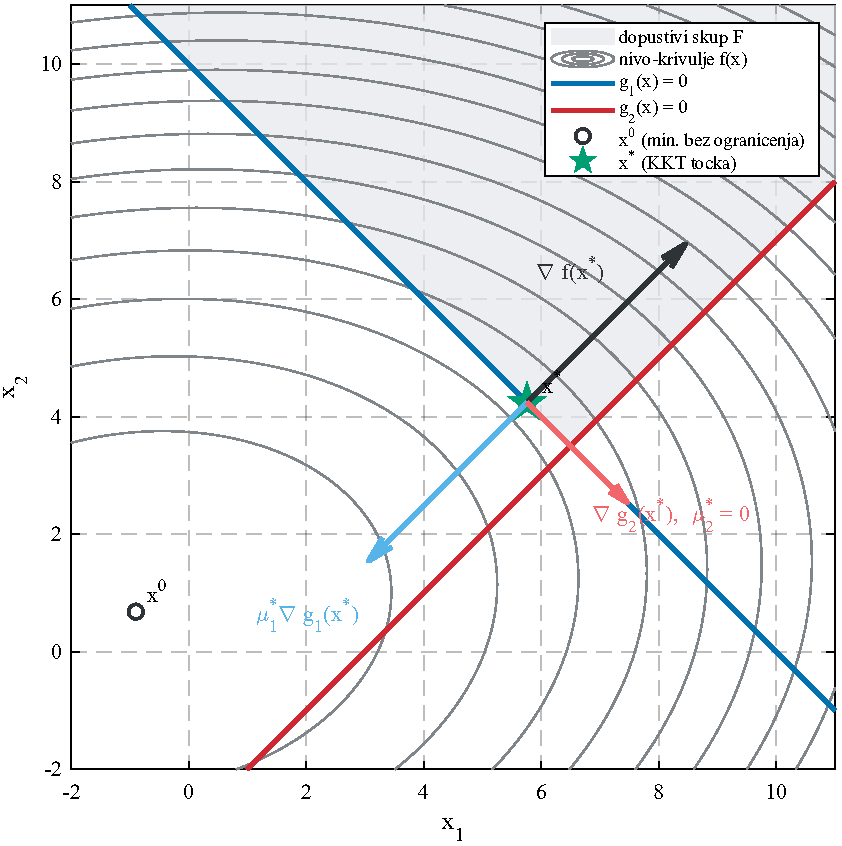
\includegraphics[width=0.92\linewidth]{../figures/fig1_1_qp_primal_geometry.pdf}
\caption{Dopustivi skup, nivo-krivulje funkcije cilja i gradijenti u KKT točki
$\xopt$ (Slika 2.1 seminara v1.2). Duljine vektora grafički su skalirane.}
\label{fig:z1c-geometrija}
\end{figure}

\subsection{Dekonstrukcija: svaki element slike posebno}

\begin{longtable}{@{}p{0.30\linewidth} p{0.66\linewidth}@{}}
\toprule
\textbf{Element} & \textbf{Što je i odakle dolazi} \\
\midrule
\endfirsthead
\toprule
\textbf{Element} & \textbf{Što je i odakle dolazi} \\
\midrule
\endhead
Osi $x_1$, $x_2$ & Prostor projektnih varijabli. Raspon je otprilike $-2$ do $11$
po obje osi, tek toliko da stanu i neograničeni minimum i KKT točka. \\[5pt]
Puna debela crta & Rub prvog ograničenja, $g_1(x) = 0$, tj.\ pravac
$x_1 + x_2 = 10$. Ide od gore lijevo prema dolje desno. \\[5pt]
Crtkano-točkasta crta & Rub drugog ograničenja, $g_2(x) = 0$, tj.\ pravac
$x_1 - x_2 = 3$. Ide od dolje lijevo prema gore desno. \\[5pt]
Sivo osjenčano područje & Dopustivi skup $\feas$: presjek poluprostora
$x_1 + x_2 \geq 10$ i $x_1 - x_2 \leq 3$. Klin koji se otvara prema gore desno,
s vrhom u $(6{,}5,\; 3{,}5)$. Neograničen je. \\[5pt]
Tanke koncentrične krivulje & Nivo-krivulje funkcije cilja. Elipse su jer je
$Q \pd 0$; središte im je u $x^{0}$, blago su nagnute i rastu prema van. \\[5pt]
Kružić, oznaka $x^{0}$ & Minimum bez ograničenja,
$x^{0} = (-0{,}898,\; 0{,}683)$. Leži \emph{izvan} sive površine --- to je
vizualni dokaz da Slučaj 1 otpada. \\[5pt]
Zvjezdica, oznaka $\xopt$ & KKT točka $(5{,}758,\; 4{,}242)$. Leži \emph{na}
punoj crti, dakle na rubu $g_1$, i to gore lijevo od vrha klina. \\[5pt]
Crna strelica iz $\xopt$ prema gore desno & $\grad f(\xopt)$, smjer $(1,1)$.
Pokazuje u smjeru rasta cilja, dakle u unutrašnjost dopustivog skupa. \\[5pt]
Siva strelica iz $\xopt$ prema dolje lijevo & $\mu_1^{\star}\grad g_1(\xopt)$,
smjer $(-1,-1)$. Točno suprotna prethodnoj --- to je slika jednadžbe
\eqref{eq:z1c-kolinearnost}. \\[5pt]
Kratka strelica desno od $\xopt$, uz oznaku $\mu_2^{\star} = 0$ & $\grad g_2$,
smjer $(1,-1)$. Nacrtana je da se vidi da postoji, ali s množiteljem nula ne
sudjeluje u ravnoteži. \\
\bottomrule
\end{longtable}

\subsection{Što slika dokazuje}

\begin{korak}[Tri zaključka koja se čitaju izravno s crteža]
\begin{enumerate}[leftmargin=*]
  \item \textbf{Zašto optimum nije $x^{0}$.} Kružić $x^{0}$ je izvan sive
        površine. Neograničeni minimum nije dopustiv, pa se rješenje mora
        pomaknuti na rub.
  \item \textbf{Zašto je optimum baš tu, a ne u vrhu.} Nivo-elipsa koja prolazi
        kroz $\xopt$ \emph{dodiruje} punu crtu --- tangentna je na nju. Kroz vrh
        $(6{,}5,\, 3{,}5)$ prolazi elipsa \emph{veće} razine, koja rub siječe. Da
        siječe, postojao bi pomak uzduž ruba koji ostaje dopustiv i smanjuje
        cilj; upravo taj pomak vodi od vrha do $\xopt$.
  \item \textbf{Zašto su KKT uvjeti zadovoljeni.} Dvije glavne strelice leže na
        istom pravcu i suprotno su usmjerene. To je geometrijski oblik uvjeta
        $\grad f + \mu_1 \grad g_1 = 0$. Kad bi među njima bio kut različit od
        $180^\circ$, postojala bi komponenta gradijenta cilja uzduž ruba --- a
        onda bi se klizanjem uzduž ruba cilj mogao smanjiti.
\end{enumerate}
\end{korak}

\section{Kako sliku nacrtati rukom}
\label{sec:z1c-crtanje}

\begin{ploca}[Cijela slika Zadatka 1c, deset poteza]
\begin{enumerate}[leftmargin=*]
  \item \textbf{Osi.} Vodoravna $x_1$, okomita $x_2$. Označi brojeve $0$, $5$,
        $10$ na objema. Ostavi malo prostora lijevo od nule, jer ondje ide $x^{0}$.
  \item \textbf{Prvi pravac.} $x_1 + x_2 = 10$ kroz $(10,0)$ i $(0,10)$. Povuci
        ga \emph{debelo} --- to je aktivno ograničenje.
  \item \textbf{Drugi pravac.} $x_1 - x_2 = 3$ kroz $(3,0)$ i $(6{,}5,\, 3{,}5)$.
        Povuci ga crtkano.
  \item \textbf{Vrh.} Označi sjecište $(6{,}5,\; 3{,}5)$ i napiši mu koordinate.
  \item \textbf{Dopustiva strana.} Uvrsti ishodište: $g_1(0,0) = 10 > 0$ (nije
        dopustivo), $g_2(0,0) = -3 < 0$ (dopustivo). Osjenčaj klin koji se otvara
        gore desno, od vrha prema gore.
  \item \textbf{Središte elipsa.} Ucrtaj kružić u $(-0{,}9,\; 0{,}7)$ i označi
        ga $x^{0}$. Izgovori: ,,neograničeni minimum, nije dopustiv``.
  \item \textbf{Elipse.} Tri koncentrične elipse oko $x^{0}$, blago nagnute
        (oko $8^\circ$), sve veće prema van. Najveću povuci tako da \emph{dodirne}
        debeli pravac.
  \item \textbf{KKT točka.} Točka dodira te elipse i debelog pravca je $\xopt$.
        Označi je zvjezdicom i napiši $(5{,}76,\; 4{,}24)$. Naglasi da je lijevo
        od vrha.
  \item \textbf{Dvije glavne strelice.} Iz $\xopt$ jedna strelica pod
        $45^\circ$ gore desno --- to je $\grad f(\xopt)$; i jedna jednako duga
        točno suprotno, dolje lijevo --- to je $\mu_1^{\star}\grad g_1$. Obje su
        okomite na debeli pravac.
  \item \textbf{Treća strelica.} Kratka strelica u smjeru $(1,-1)$, dolje desno,
        označena $\grad g_2$, uz napomenu $\mu_2^{\star} = 0$.
\end{enumerate}
\end{ploca}

\begin{zamka}[Zamka: elipsa koja siječe umjesto da dodiruje]
Ako na ploči nacrtaš elipsu koja \emph{siječe} rub u dvije točke, sam si sebi
nacrtao proturječje --- takva slika kaže da postoji dopustiv pomak koji smanjuje
cilj. Elipsa kroz optimum mora rub dodirivati u točno jednoj točki. Ako ti se pri
crtanju to ne uspije pogoditi, reci naglas: ,,skica nije u mjerilu, ali ključno
je da je u optimumu nivo-krivulja tangentna na aktivno ograničenje``.
\end{zamka}

\begin{zamka}[Zamka: smjer gradijenta cilja]
$\grad f(\xopt)$ pokazuje \emph{u} dopustivi skup, ne iz njega. Razlog: funkcija
cilja u tom smjeru raste, a dopustivi skup se prostire prema gore desno. Ono što
pokazuje van jest $-\grad f(\xopt)$, smjer najbržeg pada --- i baš zato optimum
i jest optimum: jedini smjer u kojem bi se cilj smanjio vodi izvan dopustivog
skupa.
\end{zamka}

\section{Kako je to riješeno u seminaru}
\label{sec:z1c-seminar}

\begin{seminar}{Seminar v1.2, §2.4 --- ,,(c) Grafički prikaz``}
U KKT točki $x^*$ gradijenti funkcije cilja i funkcija ograničenja iznose
\[
\nabla f(x^*) = Q x^* + c = \begin{bmatrix} 12.242424 \\ 12.242424 \end{bmatrix}, \quad
\nabla g_1(x^*) = \begin{bmatrix} -1 \\ -1 \end{bmatrix}, \quad
\nabla g_2(x^*) = \begin{bmatrix} 1 \\ -1 \end{bmatrix},
\]
pa uvjet stacionarnosti $(\star)$ daje
\[
\nabla f(x^*) = -\mu_1^* \nabla g_1(x^*) = -\frac{404}{33} \begin{bmatrix} -1 \\ -1 \end{bmatrix}.
\]
Gradijent funkcije cilja i gradijent aktivnog ograničenja su kolinearni i
suprotnog smjera. Ograničenje $g_2$ je neaktivno ($g_2(x^*) = -1.484848 < 0$), pa
je iz $(\star\star)$ $\mu_2^* = 0$ i njegov gradijent ne ulazi u ravnotežu.

Slika 2.1 prikazuje dopustivi skup $\mathcal{F}$ (osjenčano), nivo-krivulje
funkcije cilja, minimum bez ograničenja $x^0$ i KKT točku $x^*$ s ucrtanim
gradijentima. Nivo-krivulje su elipse jer je $Q \succ 0$. Duljine vektora na
slici su grafički skalirane.
\end{seminar}

Slika je izrađena u MATLAB-u; provjera kolinearnosti ispisana je u
\texttt{docs/code/task1\_output.txt}:

\begin{lstlisting}[style=outputstyle]
grad f(x*) = [12.242424, 12.242424];  -mu1*grad g1 = [12.242424, 12.242424]
\end{lstlisting}

\section{Modelski odgovori}
\label{sec:z1c-odgovori}

\begin{pitanje}{Zašto su nivo-krivulje elipse, a ne kružnice?}
\textbf{Odgovor.} Bile bi kružnice samo da je $Q$ višekratnik jedinične matrice,
dakle da su obje svojstvene vrijednosti jednake. Ovdje su $1{,}956$ i $4{,}044$,
pa je omjer poluosi $\sqrt{4{,}044/1{,}956} \approx 1{,}44$, a osi su zakrenute
za oko $8^\circ$ jer svojstveni vektori nisu poklopljeni s koordinatnim osima ---
posljedica mješovitog člana $-0{,}3\,x_1x_2$.
\end{pitanje}

\begin{pitanje}{Što biste vidjeli na slici da je $\mu_2^{\star} > 0$?}
\textbf{Odgovor.} Optimum bi bio u vrhu klina, a $-\grad f$ bi ležao \emph{unutar}
stošca razapetog s $\grad g_1$ i $\grad g_2$, dakle bio bi njihova kombinacija s
oba pozitivna koeficijenta. Kod nas $-\grad f$ leži točno na bridu tog stošca,
uzduž $\grad g_1$, pa je drugi koeficijent nula.
\end{pitanje}

\begin{pitanje}{Kako biste sa slike provjerili da je rješenje globalno, a ne lokalno?}
\textbf{Odgovor.} Sa same slike ne bih --- globalnost ne slijedi iz crteža nego
iz konveksnosti. Slika pokazuje da je uvjet stacionarnosti zadovoljen; da je taj
uvjet i \emph{dovoljan} slijedi iz toga što je problem konveksan i što je
Slaterov uvjet zadovoljen. Slika je ilustracija, ne dokaz.
\end{pitanje}

\begin{izgovor}[Čitanje slike naglas]
,,Na apscisi je $x_1$, na ordinati $x_2$. Osjenčano je dopustivo područje,
presjek poluprostora $x_1 + x_2 \geq 10$ i $x_1 - x_2 \leq 3$; to je neograničen
klin s vrhom u šest i pol, tri i pol.

Tanke koncentrične krivulje su nivo-krivulje funkcije cilja. Elipse su jer je
matrica ku pozitivno definitna, a središte im je u neograničenom minimumu minus
nula devet, nula šest osam --- koji je, kako se vidi, izvan dopustivog područja.

Zvjezdica je KKT točka, pet zarez sedam šest, četiri zarez dva četiri. Leži na
rubu prvog ograničenja, lijevo od vrha. Nivo-elipsa kroz nju tangentna je na taj
rub.

Iz te točke izlaze dvije strelice na istom pravcu i suprotnih smjerova:
gradijent funkcije cilja, koji pokazuje u dopustivo područje, i mi jedan puta
gradijent prvog ograničenja, koji pokazuje van. Njihov zbroj je nula --- to je
uvjet stacionarnosti, sada vidljiv na slici. Treća strelica je gradijent drugog
ograničenja; ono je neaktivno, množitelj mu je nula, pa u ravnotežu ne ulazi.
Duljine strelica su skalirane radi preglednosti, uspoređujem samo smjerove.``
\end{izgovor}

\chapter{Zadatak 1d --- rješenje u MATLAB-u}
\label{ch:z1-matlab}

\section{Što se ovdje traži}

Riješiti isti problem rješavačem i \emph{usporediti} dobivene primarne i dualne
varijable s analitičkim rezultatom iz (b). Naglasak je na usporedbi --- sam
poziv funkcije nije poanta.

\begin{zadatak}{Zadatak 1, podzadatak d)}
d) Riješite problem u MATLABu (quadprog i/ili yalmip) --- odredite primarne i
dualne varijable u optimumu te ih usporedite s rezultatima (Lagrangeovim
množiteljima) iz (b).
\end{zadatak}

\begin{predznanje}
\begin{itemize}[nosep,leftmargin=*]
  \item Standardni oblik QP-a $\min \tfrac12 x\trans Qx + c\trans x$ uz $Gx \leq h$ --- \S\ref{sec:z1-standardni-oblik}.
  \item Matrice $Q$, $c$, $G$, $h$ --- \eqref{eq:z1-Qc} i \eqref{eq:z1-Gh}.
  \item Analitičko rješenje s kojim se uspoređuje --- \eqref{eq:z1b-rjesenje}.
\end{itemize}
\end{predznanje}

\section{Zašto \texttt{quadprog} traži baš te argumente}
\label{sec:z1d-sucelje}

Sučelje funkcije je
\begin{center}
\texttt{quadprog(H, f, A, b, Aeq, beq, lb, ub, x0, options)}
\end{center}
i minimizira $\tfrac12 x\trans H x + f\trans x$ uz $Ax \leq b$. To je \emph{točno}
standardni oblik s Predavanja 5, pa se matrice predaju izravno, bez ikakve
pretvorbe:
\begin{equation}
\texttt{H} = Q, \quad \texttt{f} = c, \quad \texttt{A} = G, \quad \texttt{b} = h .
\end{equation}

\begin{zamka}[Zamka: MATLAB-ov $\tfrac12$ i ,,zaboravljeni`` faktor]
\texttt{quadprog} \emph{sam} podrazumijeva faktor $\tfrac12$ ispred kvadratnog
člana. Ako se preda matrica bez tog faktora --- dakle
$\begin{bsmallmatrix}1 & -0{,}15\\ -0{,}15 & 2\end{bsmallmatrix}$ umjesto $Q$ ---
rješavač će riješiti dvostruko manji kvadratni član i vratiti krivi optimum. Ovo
je najčešća pogreška pri prvom pozivu, a ne javlja se kao greška nego kao
naizgled uredan, ali pogrešan rezultat. Kontrola: usporedi
\texttt{fval} s $f(\xopt)$ izračunatim ručno.
\end{zamka}

\begin{zamka}[Zamka: $h$, a ne $-h$]
Sučelje traži $Ax \leq b$, dakle desnu stranu \emph{prije} prebacivanja. Naš
$h = (-10,\; 3)$ ide izravno. Ako se preda $(10,\, -3)$, dopustivi skup je
zrcaljen i rješenje je besmisleno.
\end{zamka}

\section{Kako je to izgledalo na vježbama}
\label{sec:z1d-vjezbe}

\begin{izvor}{Vježbe 3 --- Primjer 2, slajd 25/36 (PDF str.~30)}
\slajd[0.86]{v3-primjer2-quadprog}

\textbf{Što je na slajdu.} Snimka MATLAB-ove sesije: poziv \texttt{quadprog} za
profesorov primjer, s ispisanim rješenjem i množiteljima. Kod je strukturno
identičan našemu --- definiraju se $Q$, $c$, $G$, $h$, pa se pozove rješavač.

\textbf{Što iz toga treba zapamtiti:} profesor \emph{pokazuje kod na slajdu}.
Znači da se na obrani očekuje da znaš objasniti svaki argument poziva, a ne samo
rezultat.
\end{izvor}

\begin{izvor}{Vježbe 3 --- Primjer 2, slajd 28/36 (PDF str.~33)}
\slajd[0.86]{v3-primjer2-yalmip}

\textbf{Što je na slajdu.} Isti problem riješen preko YALMIP-a, koji kao rješavač
koristi \texttt{quadprog}. Varijable se deklariraju sa \texttt{sdpvar},
ograničenja se skupljaju u listu, pa se pozove \texttt{optimize}.

\textbf{Zašto to zadatak spominje kao alternativu:} YALMIP je modelirajući sloj,
ne rješavač. Za problem koji je već u standardnom obliku ne donosi ništa; postaje
nezamjenjiv u Zadatku 4, gdje ograničenja nisu $Gx \leq h$ nego matrične
nejednakosti.
\end{izvor}

\section{Kod i stvarni ispis}
\label{sec:z1d-kod}

\begin{seminar}{Seminar v1.2, §2.5 --- ,,(d) Numeričko rješenje u MATLAB-u``}
Problem se u MATLAB-u rješava funkcijom \texttt{quadprog}, koja minimizira
$\tfrac{1}{2}x^{\mathsf{T}}Qx + c^{\mathsf{T}}x$ uz $Gx \leq h$, pa se matrice
predaju izravno.

\begin{lstlisting}[style=matlabstyle]
Q = [2.0, -0.3; -0.3, 4.0];
c = [2.0; -3.0];
G = [-1.0, -1.0; 1.0, -1.0];
h = [-10.0; 3.0];

opts = optimoptions('quadprog', 'Display', 'none', ...
                    'Algorithm', 'interior-point-convex');
[x_qp, f_qp, ef_qp, ~, lam_qp] = quadprog(Q, c, G, h, [], [], [], [], [], opts);
\end{lstlisting}

\begin{lstlisting}[style=outputstyle]
exitflag        = 1
x_opt           = [5.757576; 4.242424]
p*  = fval      = 60.606061
lambda.ineqlin  = [12.242424; 0.000000]
\end{lstlisting}

Primarne i dualne varijable dobivene rješavačem podudaraju se s analitičkim
rezultatom do na tolerancije rješavača. Polje \texttt{lambda.ineqlin} sadrži
upravo Lagrangeove množitelje $\mu_1^*$ i $\mu_2^*$ iz KKT uvjeta.
\end{seminar}

\subsection{Što koji redak znači}

\begin{longtable}{@{}p{0.30\linewidth} p{0.66\linewidth}@{}}
\toprule
\textbf{Redak} & \textbf{Značenje} \\
\midrule
\endhead
\texttt{'Display','none'} & Isključuje ispis rješavača, jer se sve što treba
ispisuje ručno. \\[5pt]
\texttt{'Algorithm','interior-\allowbreak point-convex'} & Metoda unutarnje točke
za konveksne QP-ove. Ne nabraja aktivne skupove kao mi u (b), nego se optimumu
približava iznutra i aktivni skup ,,otkriva`` u limesu. Zato su
$\mu_2^{\star}$ i $g_2$ jednaki nuli tek do na toleranciju. \\[5pt]
\texttt{ef\_qp} (\texttt{exitflag}) & $1$ znači da je rješavač konvergirao.
Svaka druga vrijednost čini rezultat neupotrebljivim i mora se provjeriti prije
nego se brojke uopće pogledaju. \\[5pt]
\texttt{lam\_qp.ineqlin} & Vektor Lagrangeovih množitelja ograničenja
nejednakosti --- upravo $\mu$ iz KKT sustava. Postoje i polja
\texttt{eqlin}, \texttt{lower}, \texttt{upper} za ostale vrste ograničenja; ovdje
su prazna. \\[5pt]
\texttt{\textasciitilde} kao četvrti izlaz & Preskočeni izlaz
\texttt{output} (statistika iteracija), koji nam ne treba. \\
\bottomrule
\end{longtable}

\section{Usporedba, koja je zapravo zadatak}
\label{sec:z1d-usporedba}

\begin{seminar}{Seminar v1.2, Tablica 2.2}
\begin{center}
\begin{tabular}{lccc}
\toprule
\textbf{Veličina} & \textbf{Analitički} & \texttt{quadprog} & \textbf{Odstupanje} \\
\midrule
$x_1^*$   & $190/33 = 5.757576$  & $5.757576$  & $< 10^{-10}$ \\
$x_2^*$   & $140/33 = 4.242424$  & $4.242424$  & $< 10^{-10}$ \\
$\mu_1^*$ & $404/33 = 12.242424$ & $12.242424$ & $< 10^{-10}$ \\
$\mu_2^*$ & $0$                  & $0$         & --- \\
$p^*$     & $2000/33 = 60.606061$& $60.606061$ & $< 10^{-10}$ \\
\bottomrule
\end{tabular}
\end{center}
\end{seminar}

Iz punog ispisa programa vidi se i norma razlike:

\begin{lstlisting}[style=outputstyle]
|x_qp - x_analiticki| = 7.155e-11
\end{lstlisting}

\begin{korak}[Što se ovom usporedbom zapravo pokazalo]
\begin{enumerate}[leftmargin=*]
  \item Analitičko rješavanje KKT sustava i numerički rješavač daju istu točku ---
        dakle nijedan od dva puta nema grešku.
  \item Množitelji koje vraća rješavač \emph{jesu} KKT množitelji. To nije
        samorazumljivo: rješavač ih ne računa iz naše tablice slučajeva, nego kao
        dualne varijable svoje metode unutarnje točke. Da se poklapaju, potvrda
        je da su oba pristupa opis istog matematičkog objekta.
  \item Odstupanje reda $10^{-11}$ je tolerancija rješavača, a ne fizikalna
        veličina. Zato se u seminaru rezultat navodi kao razlomak, s decimalama
        u zagradi.
\end{enumerate}
\end{korak}

\section{Modelski odgovori}
\label{sec:z1d-odgovori}

\begin{pitanje}{Zašto \texttt{quadprog} vraća $\mu_2 = 0$, a ne neki mali broj poput $10^{-12}$?}
\textbf{Odgovor.} Vraća ga do na toleranciju; ispisan je kao \texttt{0.000000}
jer se ispisuje na šest decimala. Metoda unutarnje točke u limesu tjera umnožak
$\mu_j g_j$ prema nuli, pa za neaktivno ograničenje $\mu_j$ pada prema nuli
zajedno s parametrom barijere. Da je algoritam bio tipa aktivnog skupa,
$\mu_2$ bi bio točno nula po konstrukciji.
\end{pitanje}

\begin{pitanje}{Biste li isti rezultat dobili preko YALMIP-a?}
\textbf{Odgovor.} Da. YALMIP je modelirajući sloj --- problem se zapiše
deklarativno, a on ga proslijedi rješavaču, među ostalim i \texttt{quadprog}-u.
Za ovako mali QP nema razlike u rezultatu; YALMIP se isplati kad ograničenja nisu
u standardnom obliku, kao u Zadatku 4, gdje se rješavaju linearne matrične
nejednakosti.
\end{pitanje}

\begin{pitanje}{Što ako \texttt{exitflag} nije 1?}
\textbf{Odgovor.} Tada se rezultat ne smije koristiti. Vrijednost $-2$ znači da
problem nije dopustiv, $-3$ da je neograničen, $0$ da je premašen broj
iteracija. Ovdje unaprijed znamo da je problem dopustiv (Slaterova točka) i
ograničen odozdo (koercivnost), pa bi svaka od tih vrijednosti značila grešku u
predaji matrica.
\end{pitanje}

\begin{izgovor}
,,U MATLAB-u sam koristio \texttt{quadprog}, jer njegovo sučelje već jest
standardni oblik s predavanja --- minimizira jedna polovina iks transponirano ha
iks plus ef transponirano iks uz a iks manje ili jednako be --- pa sam matrice
predao izravno, bez pretvorbe. Bitno je da faktor jedna polovina rješavač
podrazumijeva, pa se predaje puna matrica ku.

Rješavač je vratio iks pet zarez sedam pet sedam pet sedam šest i četiri zarez
dva četiri dva četiri, optimalnu vrijednost šezdeset zarez šest nula šest, i
množitelje dvanaest zarez dva četiri i nulu. To se s analitičkim rješenjem iz
podzadatka b) poklapa do na jedanaestu decimalu.

Time je pokazano i nešto više od podudarnosti brojeva: polje
\texttt{lambda.ineqlin} koje rješavač vraća sadrži upravo Lagrangeove
množitelje iz KKT uvjeta, iako ih algoritam dobiva sasvim drugim putem --- kao
dualne varijable metode unutarnje točke.``
\end{izgovor}

\chapter{Zadatak 1e --- Lagrangeov dualni problem}
\label{ch:z1-dual}

\section{Što se ovdje traži}

Izvesti dualni problem \emph{analitički}, riješiti ga numerički i usporediti
dualne varijable s onima iz (b) i (d).

\begin{zadatak}{Zadatak 1, podzadatak e)}
e) Postavite i riješite Lagrangeov dualan problem (koristite MATLAB za numeričko
rješavanje dualnog problema). Usporedite vrijednost izračunatih dualnih varijabli
s onima dobivenim pod (d) i (b).
\end{zadatak}

\begin{predznanje}
\begin{itemize}[nosep,leftmargin=*]
  \item Lagrangeova funkcija \eqref{eq:z1b-lagrangian} i množitelji $\mu \geq 0$.
  \item $Q^{-1}$ postoji jer je $Q \pd 0$ --- \S\ref{sec:inverz}, \eqref{eq:alat-Q-inv}.
  \item Jaka dualnost i Slaterov uvjet --- \S\ref{sec:z1a-slater}.
  \item Značenje $\inf$ nasuprot $\min$ --- \S\ref{sec:oznake-optimizacije}.
\end{itemize}
\end{predznanje}

\section{Definicije s predavanja}
\label{sec:z1e-definicije}

\begin{izvor}{Predavanje 4 --- Lagrangeova dualnost, slajd 6/26 (PDF str.~10)}
\slajd[0.86]{p04-lagrangian-i-dual}

\textbf{Transkripcija.} \emph{Terminologija i neka svojstva.}
\begin{itemize}[nosep,leftmargin=*]
  \item Lagrangian (Lagrangeova funkcija):
        $\Lag(x,\lambda,\mu) \coloneqq f(x) + \sum_{i=1}^{m}\lambda_i h_i(x) + \sum_{j=1}^{p}\mu_j g_j(x)$
  \item Lagrangeova dualna funkcija cilja:
        $\dual(\lambda,\mu) \coloneqq \inf_x \Lag(x,\lambda,\mu)$
  \item Lagrangeov dualan problem:
        $\dopt = \sup_{\{\lambda,\mu \mid \mu \geq 0\}} \dual(\lambda,\mu)$
  \item Primarni problem: $\popt = \inf_{\{x \mid g(x) \leq 0,\, h(x) = 0\}} f(x)$
  \item $\lambda_i$ je Lagrangeov množitelj (dualna varijabla) pridružen
        ograničenju $h_i(x) = 0$;
        $\mu_j$ je Lagrangeov množitelj pridružen ograničenju $g_j(x) \leq 0$.
\end{itemize}

\textbf{Tri stvari koje treba uočiti u ovoj definiciji:}
\begin{enumerate}[nosep,leftmargin=*]
  \item Dualna funkcija nastaje \emph{minimizacijom po $x$ bez ikakvih
        ograničenja} --- ograničenja su ušla u Lagrangian i time nestala iz skupa
        po kojem se traži infimum.
  \item Dualna funkcija je \emph{uvijek konkavna}, bez obzira na to je li primarni
        problem konveksan: infimum familije afinih funkcija po $(\lambda,\mu)$ je
        konkavna funkcija. Zato je dualni problem \emph{uvijek} konveksan.
  \item Jedina preostala ograničenja u dualnom problemu su $\mu \geq 0$.
\end{enumerate}
\end{izvor}

\section{Izvod dualne funkcije za QP}
\label{sec:z1e-izvod}

\begin{izvor}{Vježbe 3 --- Primjer 2: Dualnost, KKT, osjetljivost, slajd 30/36 (PDF str.~37)}
\slajd[0.86]{v3-primjer2-dual-izvod}

\textbf{Transkripcija.} \emph{d) Postavi i riješi dualan problem.} Primaran
problem:
\[
\min_x \ \tfrac12 x\trans Qx + c\trans x \quad \text{uz ogr.} \quad Gx - h \leq 0 .
\]
Uočimo: $Q \pd 0$, pa stoga i $Q^{-1}$ postoji ($Q$ nema svojstvenu vrijednost
jednaku nuli jer su sve strogo veće od nule).
\[
\Lag(x,\mu) = \tfrac12 x\trans Qx + c\trans x + \mu\trans(Gx - h)
            = \tfrac12 x\trans Qx + (c + G\trans\mu)\trans x - \mu\trans h
\]
Dualan problem:
\[
\max_{\mu \geq 0} \ -\tfrac12 \mu\trans G Q^{-1} G\trans \mu
+ \bigl(-c\trans Q^{-1}G\trans - h\trans\bigr)\mu - \tfrac12 c\trans Q^{-1} c .
\]

\textbf{Ovo je opći rezultat za QP} --- profesor ga izvodi u simbolima, bez
brojeva, pa vrijedi i za naš zadatak. Sve što nam preostaje jest uvrstiti naše
$Q$, $c$, $G$, $h$.
\end{izvor}

\begin{korak}[Izvod, korak po korak]
\begin{enumerate}[leftmargin=*]
  \item \textbf{Grupiraj po $x$.} Uvrštavanjem $g(x) = Gx - h$ u definiciju
        Lagrangiana i skupljanjem linearnih članova:
        \[
          \Lag(x,\mu) = \tfrac12 x\trans Q x + \underbrace{(c + G\trans\mu)}_{\eqqcolon\, w}{}\trans x - \mu\trans h .
        \]
        Uveli smo kraticu $w \coloneqq c + G\trans\mu$; ona ovisi o $\mu$, ali ne o $x$.
  \item \textbf{Infimum po $x$ se \emph{postiže}.} Kako je $Q \pd 0$, funkcija
        $x \mapsto \Lag(x,\mu)$ je strogo konveksna po $x$, pa infimum nije samo
        donja granica nego se doseže u jedinstvenoj točki. Ta je točka rješenje
        uvjeta $\grad_x \Lag = 0$:
        \[
          Q\tilde{x} + w = 0 \;\Longrightarrow\; \tilde{x} = -Q^{-1}w .
        \]
  \item \textbf{Uvrsti $\tilde{x}$ natrag.} Uz $\tilde{x} = -Q^{-1}w$ i
        simetričnost $Q^{-1}$:
        \begin{align*}
          \tfrac12 \tilde{x}\trans Q \tilde{x}
            &= \tfrac12 w\trans Q^{-1} Q Q^{-1} w = \tfrac12 w\trans Q^{-1} w, \\
          w\trans \tilde{x} &= -w\trans Q^{-1} w,
        \end{align*}
        pa je
        \[
          \dual(\mu) = \tfrac12 w\trans Q^{-1}w - w\trans Q^{-1}w - \mu\trans h
                     = -\tfrac12 w\trans Q^{-1}w - \mu\trans h .
        \]
  \item \textbf{Raspiši $w = c + G\trans\mu$.}
        \[
          w\trans Q^{-1} w = c\trans Q^{-1}c + 2\,c\trans Q^{-1}G\trans\mu + \mu\trans G Q^{-1}G\trans \mu ,
        \]
        odakle
        \[
          \dual(\mu) = -\tfrac12 \mu\trans G Q^{-1}G\trans\mu
                       + \bigl(-c\trans Q^{-1}G\trans - h\trans\bigr)\mu
                       - \tfrac12 c\trans Q^{-1}c .
        \]
\end{enumerate}
\end{korak}

\begin{formula}{Dualni problem}
\begin{equation}
\max_{\mu \geq 0}\ \dual(\mu),
\qquad
\dual(\mu) = -\tfrac{1}{2}\mu\trans \underbrace{G Q^{-1} G\trans}_{\text{PSD}}\mu
+ \bigl(-c\trans Q^{-1}G\trans - h\trans\bigr)\mu
- \tfrac{1}{2}c\trans Q^{-1}c .
\label{eq:z1e-dual}
\end{equation}
Matrica $-GQ^{-1}G\trans$ je negativno semidefinitna, pa je $\dual$ konkavna
kvadratna funkcija. Maksimizacija konkavne funkcije uz ograničenje $\mu \geq 0$
je konveksan problem --- opet kvadratni program, samo u varijabli $\mu$.
\end{formula}

\section{Dualni problem u brojevima}
\label{sec:z1e-brojevi}

Uvrštavanjem $Q^{-1} = \tfrac{100}{791}\begin{bsmallmatrix}4 & 0{,}3\\ 0{,}3 & 2\end{bsmallmatrix}$,
$G$, $c$ i $h$ dobiva se, egzaktno u razlomcima:
\begin{equation}
G Q^{-1} G\trans = \frac{1}{791}\begin{bmatrix} 660 & -200 \\ -200 & 540 \end{bmatrix}
\approx \begin{bmatrix} 0{,}834387 & -0{,}252845 \\ -0{,}252845 & 0{,}682680 \end{bmatrix},
\end{equation}
\begin{equation}
-c\trans Q^{-1}G\trans - h\trans = \frac{1}{791}\begin{bmatrix} 8080 & -3623 \end{bmatrix}
\approx \begin{bmatrix} 10{,}214918 & -4{,}580278 \end{bmatrix},
\qquad
\tfrac12 c\trans Q^{-1}c = \frac{1520}{791} .
\end{equation}

\begin{korak}[Uočljiva veza: linearni član dualne funkcije]
Linearni koeficijent $-c\trans Q^{-1}G\trans - h\trans$ nije proizvoljan broj.
Vrijedi
\[
-G Q^{-1}c - h = G x^{0} - h = g(x^{0}),
\]
jer je $x^{0} = -Q^{-1}c$ neograničeni minimum iz Slučaja 1. Doista, prva
komponenta je $8080/791 = 10{,}214918$ --- upravo vrijednost $g_1(x^{0})$ zbog
koje je Slučaj 1 odbačen (\S\ref{sec:z1b-slucaj1}). Dualna funkcija u nuli ima
nagib jednak vrijednostima ograničenja u neograničenom minimumu.
\end{korak}

\begin{korak}[Provjera: $\dual(\muopt) = \popt$]
Uz $\muopt = (404/33,\; 0)$ druga komponenta ne doprinosi, pa je
\[
\dual(\muopt) = -\frac12 \cdot \frac{660}{791}\left(\frac{404}{33}\right)^{2}
+ \frac{8080}{791}\cdot\frac{404}{33} - \frac{1520}{791}
= \frac{2000}{33} = 60{,}606061 .
\]
To je točno $\popt$ iz \eqref{eq:z1b-rjesenje}: dualni procjep je \textbf{egzaktno
nula}, kako i mora biti kad vrijedi jaka dualnost.
\end{korak}

\subsection{Zašto je maksimum na rubu $\mu_2 = 0$}

\begin{korak}
Da nema ograničenja $\mu \geq 0$, maksimum konkavne kvadratne funkcije
\eqref{eq:z1e-dual} bio bi u stacionarnoj točki
$\bar{\mu} = (GQ^{-1}G\trans)^{-1}\bigl(-GQ^{-1}c - h\bigr)$. Izračunato:
\begin{equation}
\bar{\mu} = \begin{bmatrix} 23/2 \\ -49/20 \end{bmatrix}
          = \begin{bmatrix} 11{,}50 \\ -2{,}45 \end{bmatrix}.
\end{equation}
To su \emph{točno} množitelji koje smo dobili u Slučaju 4
(\S\ref{sec:z1b-slucaj4}). Druga komponenta je negativna, dakle
$\bar{\mu}$ nije dopustiv za dualni problem, pa se maksimum postiže na rubu
$\mu_2 = 0$. Ondje je
\begin{equation}
\grad \dual(\muopt) = \begin{bmatrix} 0 \\ -49/33 \end{bmatrix}
                     = \begin{bmatrix} g_1(\xopt) \\ g_2(\xopt) \end{bmatrix},
\end{equation}
što je opće svojstvo: gradijent dualne funkcije jednak je vrijednostima
ograničenja u pripadnom $\tilde{x}(\mu)$. Prva komponenta je nula jer je $g_1$
aktivno; druga je negativna, pa bi povećanje $\mu_2$ smanjilo $\dual$ --- rub je
optimalan.
\end{korak}

\begin{pojam}{Ista činjenica, tri lica}
Slučaj 4 KKT sustava, unutarnji maksimum dualne funkcije i vrh dopustivog skupa
tri su opisa iste točke $(11{,}5,\; -2{,}45)$. U primarnom svijetu odbacuje se
zbog $\mu_2 < 0$; u dualnom, zato što je izvan dopustivog skupa $\mu \geq 0$.
Ako to na obrani povežeš, pokazao si da razumiješ dualnost, a ne da si zapamtio
dva odvojena računa.
\end{pojam}

\section{Kako je to riješeno u seminaru}
\label{sec:z1e-seminar}

\begin{seminar}{Seminar v1.2, §2.6 --- ,,(e) Lagrangeov dualni problem``}
Budući da je $Q \succ 0$, matrica $Q^{-1}$ postoji, a Lagrangeova funkcija
\[
\mathcal{L}(x, \mu) = \tfrac{1}{2} x^{\mathsf{T}} Q x + (c + G^{\mathsf{T}}\mu)^{\mathsf{T}} x - \mu^{\mathsf{T}} h
\]
strogo je konveksna po $x$. Infimum se postiže u točki u kojoj je
$\nabla_x \mathcal{L} = 0$:
\[
Q\tilde{x} + c + G^{\mathsf{T}} \mu = 0 \implies \tilde{x} = -Q^{-1}(c + G^{\mathsf{T}} \mu).
\]
Uvrštavanjem $\tilde{x}$ natrag u $\mathcal{L}$ dobiva se dualna funkcija
\[
\theta(\mu) = \inf_{x} \mathcal{L}(x, \mu)
= -\tfrac{1}{2} \mu^{\mathsf{T}} G Q^{-1} G^{\mathsf{T}} \mu
+ \left( -c^{\mathsf{T}} Q^{-1} G^{\mathsf{T}} - h^{\mathsf{T}} \right) \mu
- \tfrac{1}{2} c^{\mathsf{T}} Q^{-1} c,
\]
a dualni problem glasi $\max_{\mu \geq 0} \theta(\mu)$.

Matrica $-G Q^{-1} G^{\mathsf{T}}$ je negativno semidefinitna, pa je $\theta$
konkavna kvadratna funkcija, a dualni problem je maksimizacija konkavne funkcije
uz konveksna ograničenja, dakle konveksan optimizacijski problem. Riječ je opet o
kvadratnom programu, samo u varijabli $\mu$, pa se rješava istom funkcijom
\texttt{quadprog} primijenjenom na $-\theta(\mu)$ uz donju granicu $\mu \geq 0$.

\begin{lstlisting}[style=matlabstyle]
Qi = inv(Q);
Hd = G*Qi*G';  Hd = 0.5*(Hd + Hd');    % Hessian dualnog QP-a
fd = (c'*Qi*G' + h')';
kd = 0.5*(c'*Qi*c);                    % konstantni clan
[mu_d, negd, ef_d] = quadprog(Hd, fd, [], [], [], [], [0;0], [], [], opts);
d_opt = -(negd + kd);
\end{lstlisting}

\begin{lstlisting}[style=outputstyle]
exitflag        = 1
mu*             = [12.242424; 0.000000]
d*  = theta(mu*)= 60.606061
dualni procjep p* - d* = 2.480e-10
\end{lstlisting}

Dualne varijable $\mu^*$ identične su Lagrangeovim množiteljima dobivenim
analitički pod (b) i onima koje je \texttt{quadprog} vratio pod (d). Kako je
Slaterov uvjet zadovoljen, vrijedi jaka dualnost, što potvrđuje i numerički
dualni procjep $p^* - d^* = 2.48 \cdot 10^{-10}$. Maksimum konkavne funkcije
$\theta$ postiže se na rubu $\mu_2 = 0$, što odgovara neaktivnosti drugog
primarnog ograničenja.
\end{seminar}

\subsection{Zašto kod izgleda baš tako}

\begin{longtable}{@{}p{0.34\linewidth} p{0.62\linewidth}@{}}
\toprule
\textbf{Redak} & \textbf{Razlog} \\
\midrule
\endhead
\texttt{Hd = 0.5*(Hd + Hd')} & Simetrizacija. Matematički je $GQ^{-1}G\trans$
simetrična, ali u aritmetici s pomičnim zarezom razlikuje se od svog transponata
u zadnjim bitovima, a \texttt{quadprog} traži simetričan ulaz. \\[5pt]
\texttt{fd = (c'*Qi*G' + h')'} & Predaje se \emph{minus} linearni član iz
\eqref{eq:z1e-dual}, jer se minimizira $-\dual$. Predznak je već ugrađen. \\[5pt]
\texttt{[0;0]} kao \texttt{lb} & Jedino ograničenje dualnog problema, $\mu \geq 0$,
zadaje se kao donja granica, ne kao redak matrice $A$. \\[5pt]
\texttt{d\_opt = -(negd + kd)} & \texttt{quadprog} vraća minimum od $-\dual$ bez
konstantnog člana, pa se konstanta vraća i predznak okreće. \\
\bottomrule
\end{longtable}

\begin{zamka}[Zamka: prešućeni konstantni član]
Konstanta $-\tfrac12 c\trans Q^{-1}c = -1520/791 \approx -1{,}9216$ ne utječe na
to \emph{gdje} je maksimum, pa je rješavaču nije potrebno predati. Ali utječe na
\emph{vrijednost} $\dopt$. Ako se zaboravi vratiti, dualni procjep ispadne
$\approx 1{,}92$ umjesto nule i cijeli zaključak o jakoj dualnosti pada.
\end{zamka}

\section{Modelski odgovori}
\label{sec:z1e-odgovori}

\begin{pitanje}{Zašto je dualni problem uvijek konveksan, čak i kad primarni nije?}
\textbf{Odgovor.} Jer je dualna funkcija infimum familije funkcija koje su afine
u $(\lambda,\mu)$: za svaki fiksni $x$, preslikavanje
$\mu \mapsto f(x) + \mu\trans g(x)$ je afino. Infimum bilo koje familije
konkavnih (ovdje afinih) funkcija je konkavan, a maksimizacija konkavne funkcije
uz $\mu \geq 0$ je konveksan problem. Konveksnost dualnog problema ne ovisi ni o
čemu u primarnome.
\end{pitanje}

\begin{pitanje}{Koliko bi iznosio dualni procjep da problem nije konveksan?}
\textbf{Odgovor.} Bio bi nenegativan, ali ne nužno nula --- vrijedila bi samo
slaba dualnost $\dopt \leq \popt$. Ovdje je nula jer je problem konveksan i
Slaterov uvjet zadovoljen. Numerički se dobiva $2{,}48 \cdot 10^{-10}$, što je
tolerancija rješavača, a ne stvaran procjep.
\end{pitanje}

\begin{pitanje}{Čemu uopće služi dualni problem ako primarni već znamo riješiti?}
\textbf{Odgovor.} Trima stvarima. Prvo, daje \emph{certifikat}: svaki dopustivi
$\mu \geq 0$ daje donju granicu na $\popt$, pa se optimalnost može dokazati bez
rješavanja primarnog problema. Drugo, dualne varijable imaju izravno inženjersko
značenje --- osjetljivost, o čemu je podzadatak (f). Treće, za velike probleme
dual može biti mnogo manji od primarnog, jer ima onoliko varijabli koliko primar
ima ograničenja.
\end{pitanje}

\begin{izgovor}
,,Lagranžijan sam grupirao po iks, pa je linearni član ce plus ge transponirano
mi. Budući da je ku pozitivno definitna, Lagranžijan je strogo konveksan po iks,
pa se infimum stvarno postiže, i to u točki iks tilda jednako minus ku inverz
puta ce plus ge transponirano mi.

Uvrštavanjem natrag dobiva se dualna funkcija: minus jedna polovina mi
transponirano ge ku inverz ge transponirano mi, plus linearni član, minus
konstanta jedna polovina ce transponirano ku inverz ce. Matrica ispred kvadratnog
člana je negativno semidefinitna, pa je dualna funkcija konkavna, i dualni
problem je maksimizacija konkavne funkcije uz mi veće ili jednako nuli --- dakle
opet kvadratni program.

Riješio sam ga u MATLAB-u i dobio mi jednako dvanaest zarez dva četiri i nula,
identično množiteljima iz podzadataka b) i d), s optimalnom vrijednošću šezdeset
zarez šest nula šest. Dualni procjep je dva puta deset na minus deset, dakle
numerička nula --- u skladu s jakom dualnošću.

Zanimljivo je da bi bezuvjetni maksimum dualne funkcije bio u jedanaest i pol,
minus dva zarez četiri pet. To su točno množitelji iz slučaja u kojem su oba
ograničenja aktivna, a odbacili smo ga upravo zato što je drugi množitelj
negativan. Ista činjenica, gledana iz primarnog i iz dualnog problema.``
\end{izgovor}

\chapter{Zadatak 1f --- osjetljivost optimalne vrijednosti}
\label{ch:z1-osjetljivost}

\section{Što se ovdje traži}

Odgovoriti koliko se optimalna vrijednost mijenja ako se ograničenja malo
pomaknu --- i to obrazložiti, ne samo navesti broj.

\begin{zadatak}{Zadatak 1, podzadatak f)}
f) Što možete reći o osjetljivosti optimalne vrijednosti ($p^\star =$ opt.\
vrijednost primarnog problema) na perturbacije u ograničenjima (na perturbacije
koeficijenata $b_1$ i $b_2$)?
\end{zadatak}

\begin{zamka}[Prvo razjasniti: što su $b_1$ i $b_2$]
U tekstu zadatka slovo $b$ se prije podzadatka f) nigdje ne pojavljuje ---
ograničenja su zapisana s koeficijentima $a_{ij}$ i brojevima $-10$ i $3$ na
desnoj strani. Iz konteksta su $b_1$ i $b_2$ upravo te desne strane:
\begin{equation}
b_1 = -10, \qquad b_2 = 3, \qquad\text{dakle}\qquad h = \begin{bmatrix} b_1 \\ b_2 \end{bmatrix}.
\end{equation}
,,Perturbacija koeficijenata $b_1$ i $b_2$`` znači pomicanje tih desnih strana,
tj.\ stezanje ili popuštanje ograničenja. To je tumačenje, ne citat --- na
obrani ga izgovori kao svoje tumačenje.
\end{zamka}

\begin{predznanje}
\begin{itemize}[nosep,leftmargin=*]
  \item Optimalni množitelji $\muopt = (404/33,\; 0)$ --- \eqref{eq:z1b-rjesenje}.
  \item Jaka dualnost vrijedi (Slater) --- \S\ref{sec:z1a-slater}.
  \item Perturbacijski vektor $v$ --- \S\ref{sec:oznake-optimizacije}.
  \item Rezerva neaktivnog ograničenja, $g_2(\xopt) = -49/33$ --- \S\ref{sec:z1b-slucaj2}.
\end{itemize}
\end{predznanje}

\section{Perturbirani problem}
\label{sec:z1f-perturbirani}

\begin{izvor}{Predavanje 4 --- Lagrangeova dualnost, slajd 23/26 (PDF str.~31)}
\slajd[0.86]{p04-perturbirani-problem}

\textbf{Transkripcija.} \emph{Perturbiran optimizacijski problem.}
\[
\begin{aligned}
\text{Primaran:} \quad \min_x \ & f(x) \\
\text{uz ogr.} \quad & h_i(x) = u_i, && i = 1, \dots, m \\
& g_j(x) \leq v_j, && j = 1, \dots, p
\end{aligned}
\qquad
\begin{aligned}
\text{Dualan:} \quad \max_{\lambda,\mu} \ & \dual(\lambda,\mu) - \lambda\trans u - \mu\trans v \\
\text{uz ogr.} \quad & \mu \geq 0
\end{aligned}
\]
$u = [u_1 \dots u_m]\trans$, $v = [v_1 \dots v_p]\trans$ su perturbacijski
parametri. Neka je $\popt(u,v)$ opt.\ vrijednost primarnog problema, kao funkcija
od $u$ i $v$; $\popt(0,0)$ je optimalna vrijednost neperturbiranog primarnog
problema.

\textbf{Ključna zapažanja:}
\begin{itemize}[nosep,leftmargin=*]
  \item Perturbacija ulazi na \emph{desnu} stranu ograničenja. $v_j > 0$
        \emph{popušta} $j$-to ograničenje (dopustivi skup raste), $v_j < 0$ ga
        \emph{steže}.
  \item Dualni problem se mijenja samo za dodatni linearni član $-\mu\trans v$ ---
        i baš zato je veza između $\mu$ i osjetljivosti tako izravna.
\end{itemize}
\end{izvor}

Za naš zadatak, s $g(x) = Gx - h$, perturbirani problem glasi
\begin{equation}
\popt(v) = \min\left\{ \tfrac12 x\trans Q x + c\trans x \ \middle|\ Gx - h \leq v \right\},
\label{eq:z1f-perturbirani}
\end{equation}
a to je isto što i pomicanje desnih strana s $h$ na $h + v$, dakle
$b_1 \to b_1 + v_1$ i $b_2 \to b_2 + v_2$.

\section{Globalna granica}
\label{sec:z1f-globalna}

\begin{izvor}{Predavanje 4 --- Lagrangeova dualnost, slajd 25/26 (PDF str.~33)}
\slajd[0.86]{p04-globalna-osjetljivost}

\textbf{Transkripcija.} Iz $\popt(u,v) \geq \popt(0,0) - \lambda^{\star\mathsf{T}}u - \mu^{\star\mathsf{T}}v$
slijede implikacije:
\begin{itemize}[nosep,leftmargin=*]
  \item ako je $\mu_j^{\star}$ \textbf{velik}: $\popt$ znatno raste ako
        ,,stisnemo`` ograničenje $g_j(x) \leq 0$ na $g_j(x) \leq v_j$ gdje je $v_j < 0$;
  \item ako je $\mu_j^{\star}$ \textbf{malen}: $\popt$ se ne smanjuje znatno ako
        ,,relaksiramo`` ograničenje na $g_j(x) \leq v_j$ gdje je $v_j > 0$.
\end{itemize}
(Slajd navodi i analogne implikacije za množitelje $\lambda_i$ ograničenja
jednakosti, kojih u našem zadatku nema.)

\textbf{Zašto je ovo \emph{globalna} tvrdnja:} ovo je nejednakost, ne
aproksimacija, i vrijedi za \emph{svaku} veličinu perturbacije --- ne samo za
malu. Cijena je što daje samo jednostranu granicu.
\end{izvor}

\begin{formula}{Globalna donja granica}
\begin{equation}
\popt(v) \;\geq\; \popt(0) - \muopt{}\trans v
\qquad\text{za svaki } v .
\label{eq:z1f-globalna}
\end{equation}
Uz $\muopt = (404/33,\; 0)$ i $\popt(0) = 2000/33$:
\begin{equation}
\popt(v) \;\geq\; \frac{2000}{33} - \frac{404}{33}\,v_1 .
\end{equation}
\end{formula}

\section{Lokalna osjetljivost}
\label{sec:z1f-lokalna}

\begin{izvor}{Predavanje 4 --- Lagrangeova dualnost, slajd 26/26 (PDF str.~34)}
\slajd[0.86]{p04-lokalna-osjetljivost}

\textbf{Transkripcija.} \emph{Lokalna osjetljivost.} Pretpostavimo jaku dualnost
za neperturbiran problem i neka su $\lambda^{\star}$, $\muopt$ optimalne dualne
varijable primarnog problema. Ako je $\popt(u,v)$ diferencijabilno u $(0,0)$,
tada vrijedi
\[
\lambda_i^{\star} = -\frac{\partial \popt(0,0)}{\partial u_i},
\qquad
\mu_i^{\star} = -\frac{\partial \popt(0,0)}{\partial v_i}.
\]

\textbf{Dvije pretpostavke koje se ne smiju prešutjeti:} jaka dualnost (kod nas
osigurana Slaterovim uvjetom) i \emph{diferencijabilnost} $\popt$ u nuli. Druga
zna pasti --- $\popt(v)$ je konveksna po $v$, ali može imati lom ondje gdje se
mijenja aktivni skup.
\end{izvor}

\begin{formula}{Osjetljivost --- ,,cijena u sjeni``}
\begin{equation}
\left.\frac{\partial \popt}{\partial v_i}\right|_{v = 0} = -\mu_i^{\star} .
\label{eq:z1f-osjetljivost}
\end{equation}
Lagrangeov množitelj je, do na predznak, \textbf{cijena} $i$-tog ograničenja:
koliko se optimalna vrijednost popravi po jedinici popuštanja.
\end{formula}

\begin{korak}[Brojevi za naš zadatak]
Uz $\muopt = (404/33,\; 0)$:
\begin{equation}
\frac{\partial \popt}{\partial v_1} = -\frac{404}{33} = -12{,}242424,
\qquad
\frac{\partial \popt}{\partial v_2} = 0 .
\end{equation}
Čitanje:
\begin{itemize}[leftmargin=*]
  \item \textbf{Prvo ograničenje.} Popuštanje za $\Delta b_1 > 0$ smanjuje
        $\popt$ za približno $12{,}2424 \cdot \Delta b_1$. Stezanje ga za isto
        toliko povećava. Ovo je ograničenje koje ,,stoji`` --- ono drži rješenje.
  \item \textbf{Drugo ograničenje.} U prvom redu nema nikakvog utjecaja, jer je
        $g_2$ u optimumu neaktivno pa je $\mu_2^{\star} = 0$. Optimum ga
        jednostavno ne dodiruje.
\end{itemize}
\end{korak}

\subsection{Dokle vrijedi ,,nema utjecaja``}

\begin{korak}[Rezerva do promjene aktivnog skupa]
Tvrdnja $\partial\popt/\partial v_2 = 0$ vrijedi samo dok $g_2$ ostaje neaktivno.
Rezerva iznosi
\begin{equation}
\abs{g_2(\xopt)} = \frac{49}{33} = 1{,}484848 .
\end{equation}
Ako se drugo ograničenje stegne za više od toga --- dakle $v_2 < -49/33$ ---
ono postaje aktivno, aktivni skup se mijenja, $\mu_2$ postaje pozitivan, i od tog
trenutka perturbacija \emph{jest} skupa. Baš na toj granici $\popt(v)$ ima lom i
nije diferencijabilna, pa pretpostavka s Predavanja 4 prestaje vrijediti.
\end{korak}

\begin{zamka}[Zamka: ,,$\mu_2 = 0$ znači da ograničenje ne treba``]
Ne znači. Ograničenje $g_2$ i dalje je dio problema i i dalje omeđuje dopustivi
skup. Znači samo da u \emph{ovom} optimumu nije aktivno, pa infinitezimalna
promjena njegove desne strane ne mijenja rješenje. Za promjenu veću od rezerve
$1{,}4848$ ograničenje postaje ono koje veže. Reci to eksplicitno --- to je
razlika između odgovora i naučenog odgovora.
\end{zamka}

\begin{zamka}[Zamka: predznak]
Formula ima minus: $\partial\popt/\partial v_i = -\mu_i^{\star}$, a $\mu_i^{\star} \geq 0$,
pa je derivacija $\leq 0$. Smisao: popuštanje ograničenja ($v_i > 0$) povećava
dopustivi skup, a minimum po većem skupu ne može biti veći. Ako ti u odgovoru
ispadne da popuštanje \emph{povećava} $\popt$, negdje si izgubio predznak.
\end{zamka}

\section{Numerička provjera}
\label{sec:z1f-provjera}

\begin{seminar}{Seminar v1.2, §2.7 --- ,,(f) Osjetljivost optimalne vrijednosti``}
Perturbacija desnih strana ograničenja uvodi se vektorom $v = [v_1, v_2]^{\mathsf{T}}$:
\[
p^*(v) = \min \left\{ \tfrac{1}{2} x^{\mathsf{T}} Q x + c^{\mathsf{T}} x \ \middle| \ Gx - h \leq v \right\},
\]
pri čemu $v_i$ odgovara pomaku desne strane $b_i$ $i$-tog ograničenja. Za
konveksan problem sa zadovoljenim Slaterovim uvjetom vrijedi
\[
\frac{\partial p^*}{\partial v_i}\bigg|_{v = 0} = -\mu_i^*.
\]
Uz $\mu^* = [404/33,\ 0]^{\mathsf{T}}$ slijedi
\[
\frac{\partial p^*}{\partial v_1} = -\frac{404}{33} = -12.242424, \qquad
\frac{\partial p^*}{\partial v_2} = 0.
\]
Optimalna vrijednost osjetljiva je samo na perturbaciju prvog ograničenja:
opuštanje ograničenja $g_1$ za $\Delta b_1 > 0$ smanjuje $p^*$ za približno
$12.2424 \, \Delta b_1$. Perturbacija drugog ograničenja nema utjecaja u prvom
redu jer je $g_2$ u optimumu neaktivno, tj.\ $\mu_2^* = 0$; to vrijedi sve dok je
perturbacija dovoljno mala da se aktivni skup ne promijeni (rezerva do aktivacije
iznosi $|g_2(x^*)| = 1.484848$).

\begin{lstlisting}[style=matlabstyle]
dlt = 1e-4;
[~, f_v1] = quadprog(Q, c, G, h + [dlt; 0], [], [], [], [], [], opts);
[~, f_v2] = quadprog(Q, c, G, h + [0; dlt], [], [], [], [], [], opts);
dp1 = (f_v1 - f_qp)/dlt;
dp2 = (f_v2 - f_qp)/dlt;
\end{lstlisting}

\begin{lstlisting}[style=outputstyle]
dp*/dv1 numericki = -12.242364,  -mu1* = -12.242424,  odstupanje = 5.99e-05
dp*/dv2 numericki = 0.000000,  -mu2* = 0.000000,  odstupanje = 0.00e+00
\end{lstlisting}

Jednostrana numerička derivacija odstupa od $-\mu_1^*$ za $5.99 \cdot 10^{-5}$,
što je reda veličine samog koraka $\delta$ i u skladu s teorijskim rezultatom.
\end{seminar}

\begin{korak}[Zašto odstupanje nije nula]
Korištena je \emph{jednostrana} razlika, $\bigl(\popt(\delta) - \popt(0)\bigr)/\delta$,
čija je pogreška reda $O(\delta)$. Uz $\delta = 10^{-4}$ očekuje se odstupanje
reda $10^{-4}$ do $10^{-5}$ --- dobiveno je $5{,}99\cdot 10^{-5}$, dakle točno
onoliko koliko metoda daje. Da je korištena centralna razlika,
$\bigl(\popt(\delta) - \popt(-\delta)\bigr)/(2\delta)$, pogreška bi bila $O(\delta^2)$.
Odstupanje, dakle, nije greška u teoriji nego svojstvo odabrane numeričke sheme.
\end{korak}

\section{Isti podzadatak na vježbama}
\label{sec:z1f-vjezbe}

\begin{izvor}{Vježbe 3 --- Primjer 2, slajd 34/36 (PDF str.~41)}
\slajd[0.86]{v3-primjer2-osjetljivost}

\textbf{Transkripcija.} \emph{e) Što možete reći o osjetljivosti optimalne
vrijednosti na perturbacije u ograničenjima?} Budući da je
$\mu^{\star} = [0,\ 2,\ 0,\ 2]\trans$, imamo
\[
\frac{\partial \popt(0,0,0,0)}{\partial v_1} = 0,\quad
\frac{\partial \popt}{\partial v_2} = -2,\quad
\frac{\partial \popt}{\partial v_3} = 0,\quad
\frac{\partial \popt}{\partial v_4} = -2 .
\]

\textbf{Struktura odgovora je identična našoj:} pročitaj množitelje, stavi minus,
i to je cijela osjetljivost. Ograničenja s nultim množiteljem su neaktivna i ne
utječu. Razlika je samo u tome što u profesorovu primjeru \emph{dva} ograničenja
imaju množitelj različit od nule, a kod nas jedno.
\end{izvor}

\section{Modelski odgovori}
\label{sec:z1f-odgovori}

\begin{pitanje}{Što biste rekli inženjeru koji pita treba li uložiti u popuštanje ograničenja?}
\textbf{Odgovor.} Da se isplati ulagati isključivo u prvo ograničenje, i to sve
dok je cijena jedinice popuštanja manja od $12{,}24$ u jedinicama funkcije cilja.
Ulaganje u drugo ograničenje ne donosi ništa --- ono nije aktivno, pa se rješenje
ne bi pomaknulo. Množitelj je doslovno \emph{cijena u sjeni}: koliko bi platio za
jedinicu labavosti.
\end{pitanje}

\begin{pitanje}{Je li $\popt(v)$ linearna funkcija od $v$?}
\textbf{Odgovor.} Nije, nego konveksna i po dijelovima glatka. Derivacija
$-\muopt$ vrijedi lokalno, dok se aktivni skup ne promijeni. Nejednakost
$\popt(v) \geq \popt(0) - \muopt{}\trans v$ vrijedi globalno, i geometrijski
znači da je afina funkcija na desnoj strani \emph{potporna ravnina} konveksne
funkcije $\popt$ u točki $v = 0$.
\end{pitanje}

\begin{pitanje}{Kako biste odredili osjetljivost da je problem nekonveksan?}
\textbf{Odgovor.} Ovako ne bih. Izvod se oslanja na jaku dualnost, koja kod
nekonveksnih problema općenito ne vrijedi --- ostaje samo slaba dualnost, pa se
iz množitelja dobiva jednostrana granica, ne derivacija. Osjetljivost bi se onda
procjenjivala numerički, ponovnim rješavanjem perturbiranog problema, uz svijest
da rješavač može završiti u drugom lokalnom minimumu.
\end{pitanje}

\begin{izgovor}
,,Prvo bih razjasnio oznaku: $b_1$ i $b_2$ iz teksta zadatka su desne strane
ograničenja, minus deset i tri. Perturbaciju uvodim vektorom ve, tako da
ograničenja postanu ge iks minus ha manje ili jednako ve.

Budući da je problem konveksan i Slaterov uvjet zadovoljen, vrijedi jaka
dualnost, pa parcijalna derivacija optimalne vrijednosti po $v_i$ u nuli iznosi
minus mi i-to optimalno. Kod nas je mi jednak četiristo četiri kroz trideset tri i
nula, pa je osjetljivost po prvom ograničenju minus dvanaest zarez dva četiri, a
po drugom nula.

Inženjerski: samo prvo ograničenje ima cijenu. Popuštanje prvog ograničenja za
jedinicu smanjuje optimalnu vrijednost za dvanaest zarez dva četiri. Drugo
ograničenje je neaktivno, ima rezervu jedan zarez četiri osam, i sve dok
perturbacija ne premaši tu rezervu, na optimum ne utječe. Preko te granice
aktivni skup se mijenja i optimalna vrijednost ima lom.

Provjerio sam i numerički, konačnim razlikama s korakom deset na minus četiri:
dobio sam minus dvanaest zarez dva četiri dva tri šest četiri, uz odstupanje šest
puta deset na minus pet --- što je red veličine samog koraka, jer je razlika
jednostrana.``
\end{izgovor}

\chapter{Zadatak 1 --- priprema za obranu}
\label{ch:z1-obrana}

\section{Brojevi koje moraš znati napamet}
\label{sec:z1o-brojevi}

Ovo je jedina tablica u udžbeniku koju treba naučiti doslovno. Sve ostalo se
izvodi.

\begin{longtable}{@{}p{0.30\linewidth} p{0.30\linewidth} p{0.34\linewidth}@{}}
\toprule
\textbf{Veličina} & \textbf{Egzaktno} & \textbf{Decimalno} \\
\midrule
\endhead
$\lambda(Q)$ & --- & $1{,}955969$ \ i \ $4{,}044031$ \\
$\det Q$ & $791/100$ & $7{,}91$ \\
$x^{0}$ (neogr.\ min.) & $(-710/791,\; 540/791)$ & $(-0{,}897598,\; 0{,}682680)$ \\
$g_1(x^{0})$ & $8080/791$ & $10{,}214918$ \\
$\xopt$ & $(190/33,\; 140/33)$ & $(5{,}757576,\; 4{,}242424)$ \\
$\muopt$ & $(404/33,\; 0)$ & $(12{,}242424,\; 0)$ \\
$\popt = \dopt$ & $2000/33$ & $60{,}606061$ \\
$g_2(\xopt)$ (rezerva) & $-49/33$ & $-1{,}484848$ \\
$\grad f(\xopt)$ & $(404/33,\; 404/33)$ & $(12{,}242424,\; 12{,}242424)$ \\
Vrh dopustivog skupa & $(13/2,\; 7/2)$ & $(6{,}5,\; 3{,}5)$ \\
Množitelji u vrhu & $(23/2,\; -49/20)$ & $(11{,}50,\; -2{,}45)$ \\
Slaterova točka & $(7,\; 6)$ & $g_1 = -3$, $g_2 = -2$ \\
$\partial\popt/\partial v$ & $(-404/33,\; 0)$ & $(-12{,}242424,\; 0)$ \\
\bottomrule
\end{longtable}

\begin{izgovor}[Trik za pamćenje]
Sve što je važno ima nazivnik $33$. $x_1^{\star} = 190/33$, $x_2^{\star} = 140/33$,
$\mu_1^{\star} = 404/33$, $\popt = 2000/33$, rezerva $= -49/33$. Zapamti pet
brojnika --- $190$, $140$, $404$, $2000$, $-49$ --- i nazivnik $33$, i imaš cijeli
zadatak. Provjera: $190 + 140 = 330 = 10\cdot33$, što je upravo aktivno
ograničenje $x_1 + x_2 = 10$.
\end{izgovor}

\section{Zadatak u pet rečenica}
\label{sec:z1o-sazetak}

\begin{izgovor}[Ako imaš samo minutu]
,,Zadatak 1 je kvadratni program s dva ograničenja nejednakosti. Problem je
konveksan --- Hesseova matrica je pozitivno definitna, ograničenja su afina --- i
Slaterov uvjet vrijedi, pa su KKT uvjeti nužni i dovoljni.

Riješio sam KKT sustav nabrajanjem sve četiri kombinacije aktivnosti. Tri
otpadaju: jedna zbog nedopustivosti, dvije zbog negativnog množitelja. Preostaje
slučaj u kojem je aktivno samo prvo ograničenje, s rješenjem sto devedeset kroz
trideset tri i sto četrdeset kroz trideset tri.

\texttt{quadprog} daje isto do na jedanaestu decimalu, i vraća iste množitelje.

Dualni problem sam izveo analitički --- opet kvadratni program, u varijabli mi --- i
riješio numerički; dualni procjep je numerička nula, kako i mora biti uz jaku
dualnost.

Osjetljivost slijedi izravno iz množitelja: samo prvo ograničenje ima cijenu,
dvanaest zarez dva četiri po jedinici; drugo je neaktivno i nema utjecaja dok
perturbacija ne premaši rezervu od jedan zarez četiri osam.``
\end{izgovor}

\section{Pitanja koja se očekuju}
\label{sec:z1o-pitanja}

\subsection{O konveksnosti}

\begin{pitanje}{Kako biste dokazali konveksnost da funkcija cilja nije kvadratna?}
\textbf{Odgovor.} Kriterij drugog reda vrijedi i tada, samo Hessian više nije
konstantan, pa treba pokazati $\grad^2 f(x) \psd 0$ \emph{za sve $x$ u domeni}.
Ako to nije izvedivo, ostaje definicija preko tetive,
$f(\alpha x_1 + (1-\alpha)x_2) \leq \alpha f(x_1) + (1-\alpha)f(x_2)$, ili
sastavljanje funkcije od poznatih konveksnih gradivnih blokova pravilima koja ih
čuvaju --- zbroj, maksimum, kompozicija s afinim preslikavanjem.
\end{pitanje}

\begin{pitanje}{Što ako je $Q$ samo pozitivno semidefinitna, a ne definitna?}
\textbf{Odgovor.} Problem je i dalje konveksan, ali funkcija cilja nije strogo
konveksna, pa rješenje ne mora biti jedinstveno --- može postojati cijeli
optimalni segment. Osim toga, $Q^{-1}$ tada ne postoji, pa izvod dualne funkcije
iz podzadatka (e) u ovom obliku propada i treba ga voditi preko pseudoinverza,
uz uvjet dopustivosti na $c + G\trans\mu$.
\end{pitanje}

\begin{pitanje}{Zašto je bilo važno provjeriti Slaterov uvjet?}
\textbf{Odgovor.} Jer bez njega KKT uvjeti ostaju samo nužni. Iz nužnosti slijedi
da optimum \emph{ako postoji} zadovoljava KKT; ne slijedi da točka koja
zadovoljava KKT jest optimum. Slater daje jaku dualnost, a odatle i dovoljnost ---
teorem s Predavanja 4, slajd 17/26.
\end{pitanje}

\subsection{O KKT uvjetima}

\begin{pitanje}{Objasnite fizikalno uvjet komplementarnosti.}
\textbf{Odgovor.} Ograničenje koje ne dodiruje rješenje ne smije na njega ni
djelovati. Ako je $g_j(\xopt) < 0$, ograničenje je ,,daleko`` i njegova sila,
$\mu_j$, mora biti nula. Obrnuto, ako je sila različita od nule, ograničenje mora
biti aktivno --- rješenje leži na njemu. Umnožak $\mu_j g_j = 0$ zapisuje upravo
tu ekskluzivnost.
\end{pitanje}

\begin{pitanje}{Što bi značilo da je gradijent aktivnog ograničenja nul-vektor?}
\textbf{Odgovor.} Da uvjet regularnosti pada. Gradijenti aktivnih ograničenja
tada nisu linearno nezavisni, KKT teorem se ne smije primijeniti i množitelji ne
moraju postojati. Kod nas je $\grad g_1 = (-1,-1) \neq 0$, i to je jedini aktivan
gradijent, pa je linearna nezavisnost trivijalno zadovoljena.
\end{pitanje}

\begin{pitanje}{Zašto se u Slučaju 2 množitelj $\mu_1$ mogao eliminirati?}
\textbf{Odgovor.} Jer je u obje skalarne jednadžbe stacionarnosti ušao s istim
koeficijentom, $-1$, budući da su obje komponente $\grad g_1$ jednake $-1$.
Izjednačavanjem izraza za $\mu_1$ iz dviju jednadžbi množitelj ispada, i ostaje
jedna linearna veza između $x_1$ i $x_2$, koja se s uvjetom aktivnosti rješava
kao sustav $2\times2$.
\end{pitanje}

\subsection{O dualnosti}

\begin{pitanje}{Što bi značio pozitivan dualni procjep?}
\textbf{Odgovor.} Da jaka dualnost ne vrijedi --- dakle da problem nije konveksan
ili da nije zadovoljen uvjet kvalifikacije ograničenja. Kod nas je oboje
zadovoljeno, pa je procjep nula; izračunatih $2{,}48\cdot10^{-10}$ je tolerancija
rješavača.
\end{pitanje}

\begin{pitanje}{Koliko varijabli ima dualni problem?}
\textbf{Odgovor.} Onoliko koliko primar ima ograničenja --- ovdje dvije. Primar
ima dvije varijable i dva ograničenja, pa su iste veličine. Kod problema s mnogo
varijabli i malo ograničenja dual može biti bitno manji, i to je jedan od
praktičnih razloga zašto se uopće koristi.
\end{pitanje}

\subsection{O osjetljivosti}

\begin{pitanje}{Zašto u formuli osjetljivosti stoji minus?}
\textbf{Odgovor.} Zato što $v_i > 0$ popušta ograničenje i povećava dopustivi
skup, a minimum po većem skupu ne može porasti. Kako je $\mu_i^{\star} \geq 0$,
derivacija $-\mu_i^{\star}$ je nepozitivna --- popuštanje smanjuje ili ne mijenja
$\popt$.
\end{pitanje}

\begin{pitanje}{Vrijedi li rezultat za veliku perturbaciju?}
\textbf{Odgovor.} Kao derivacija --- ne, samo lokalno, dok se aktivni skup ne
promijeni. Ali globalna nejednakost
$\popt(v) \geq \popt(0) - \muopt{}\trans v$ vrijedi za svaki $v$, jer slijedi iz
slabe dualnosti primijenjene na perturbirani problem.
\end{pitanje}

\section{Popis zamki}
\label{sec:z1o-zamke}

\begin{longtable}{@{}p{0.05\linewidth} p{0.42\linewidth} p{0.47\linewidth}@{}}
\toprule
\textbf{\#} & \textbf{Zamka} & \textbf{Kako je izbjeći} \\
\midrule
\endhead
1 & Faktor $\tfrac12$ ispred kvadratne forme & Uvijek raspiši
$\tfrac12 x\trans Qx$ natrag i usporedi sa zadanom funkcijom (\S\ref{sec:kvadratna-forma}). \\[5pt]
2 & Dijeljenje mješovitog člana na pola & $Q_{12} = -0{,}3$, ne $-0{,}15$;
polovina je već u faktoru ispred. \\[5pt]
3 & Predznak pri prebacivanju $-10$ & $-x_1-x_2 \leq -10 \Leftrightarrow -x_1-x_2+10 \leq 0$
(\S\ref{sec:z1-ogranicenja}). \\[5pt]
4 & Odgovor samo o funkciji cilja & Zadatak pita je li \emph{problem} konveksan --- i
dopustivi skup mora u odgovor. \\[5pt]
5 & Zaključivanje o definitnosti iz predznaka elemenata & Samo svojstvene
vrijednosti, minori, ili $z\trans Qz$ (\S\ref{sec:relacije}). \\[5pt]
6 & Prešućena egzistencija minimuma & Skup je neograničen; treba spomenuti
koercivnost. \\[5pt]
7 & Rješavanje samo ,,pogođenog`` slučaja & Ispiši tablicu svih $2^m$ kombinacija,
kao profesor na Vježbama 3. \\[5pt]
8 & Negativan $\mu$ shvaćen kao greška u računu & To je rezultat --- dokaz da ta
kombinacija nije optimalna. \\[5pt]
9 & Zaboravljena provjera neaktivnog ograničenja & U Slučaju 2 treba pokazati i
$g_2(\xopt) < 0$. \\[5pt]
10 & Vrh dopustivog skupa uzet kao optimum & Ondje je $\mu_2 = -2{,}45 < 0$;
vrh otpada. \\[5pt]
11 & Elipsa nacrtana tako da siječe rub & U optimumu mora \emph{dodirivati}
(\S\ref{sec:z1c-crtanje}). \\[5pt]
12 & Krivi smjer $\grad f(\xopt)$ & Pokazuje \emph{u} dopustivi skup; van pokazuje
$-\grad f$. \\[5pt]
13 & Puna matrica bez $\tfrac12$ predana \texttt{quadprog}-u & Rješavač
podrazumijeva $\tfrac12$; predaje se $Q$. \\[5pt]
14 & Izostavljen konstantni član kod dualnog problema & Bez
$-\tfrac12 c\trans Q^{-1}c$ procjep ispadne $1{,}92$ umjesto nule. \\[5pt]
15 & ,,$\mu_2 = 0$ znači da ograničenje ne treba`` & Znači samo da nije aktivno;
rezerva je $1{,}4848$. \\[5pt]
16 & Izgubljen minus u osjetljivosti & Popuštanje smanjuje $\popt$; derivacija je
nepozitivna. \\
\bottomrule
\end{longtable}

\section{Redoslijed izlaganja pred pločom}
\label{sec:z1o-redoslijed}

\begin{ploca}[Kako izložiti cijeli Zadatak 1]
\begin{enumerate}[leftmargin=*]
  \item \textbf{Zapiši problem} u matričnom obliku, gore lijevo na ploči, i ostavi
        ga ondje --- na njega ćeš se pozivati cijelo vrijeme.
  \item \textbf{Konveksnost} u tri reda: $\grad^2 f = Q$, svojstvene vrijednosti
        $1{,}956$ i $4{,}044$, ograničenja afina. Dopiši Slaterovu točku $(7,6)$.
  \item \textbf{Tablica četiriju slučajeva} u desnom gornjem kutu. Prekriži tri,
        zaokruži jedan.
  \item \textbf{Slučaj 2 do kraja}: tri jednadžbe, eliminacija $\mu_1$,
        $6{,}6x_1 = 38$, rezultat. Uokviri $\xopt$ i $\muopt$.
  \item \textbf{Slika} u donjoj polovici ploče, po postupku iz
        \S\ref{sec:z1c-crtanje}. Ostavi joj dovoljno mjesta --- to je dio na kojem
        se najviše dobiva.
  \item \textbf{Dual} u dva reda: $\tilde{x} = -Q^{-1}(c + G\trans\mu)$, pa
        $\dual(\mu)$. Naglasi da je opet QP i da je $\dopt = \popt$.
  \item \textbf{Osjetljivost} u jednom redu: $\partial\popt/\partial v = -\muopt$,
        pa brojevi i rezerva.
\end{enumerate}
\end{ploca}

\begin{zamka}[Zamka: brisanje ploče]
Ne briši matrični zapis problema ni tablicu slučajeva. Ispitivač se vraća na njih
pitanjima tipa ,,a što bi bilo da je ovdje umjesto tri bilo pet``. Ako je ploča
prazna, počinješ ispočetka i gubiš vrijeme.
\end{zamka}

\section{Veze prema ostalim zadacima}
\label{sec:z1o-veze}

\begin{predznanje}
Što se iz Zadatka 1 nosi dalje:
\begin{itemize}[leftmargin=*]
  \item \textbf{U Zadatak 2}: isti problem, ali s nesigurnim koeficijentima
        $a_{ij}$. Robusna formulacija svodi se na konačno mnogo ograničenja, pa
        se opet rješava KKT uvjetima --- ista tablica aktivnosti, više redaka.
  \item \textbf{U Zadatak 3}: ista logika ,,funkcija cilja plus afina
        ograničenja``, samo je cilj $\ell_1$-norma, pa se pomoćnim varijablama
        svodi na linearni program.
  \item \textbf{U Zadatak 4}: pojam pozitivne definitnosti prelazi s Hesseove
        matrice na Ljapunovljevu matricu $P$; umjesto $Q \pd 0$ traži se
        $P \pd 0$ i $M \nd 0$, a to su linearne matrične nejednakosti.
\end{itemize}
\end{predznanje}


\end{document}
